\setchapterpreamble[u]{\margintoc}
\chapter{Machine Learning \& Computer Vision}
\labch{MLandCV}
In this chapter the theoretical backgrounds and motivation of neural networks ought to be explored.

First, a physical/biological motivation will set the foundation for the theoretical background accompanied by a more mathematical motivation later on.
Thereafter, more advanced lines of thought will be introduced that finally lead to convolutional neural networks as the current driving force in computer vision.

\section{Artificial Neural Networks}
\labsec{ANN}

\subsection[Inspiration]{Neurobiological Inspiration}

Many human achievements have at least been partially inspired by studying nature.
A very popular example is that of airplanes and birds.
By studying how birds can fly, people found out that the shape of their wings is essential.
Inventors and engineers have taken this as inspiration and slowly but steadily came up with planes and the like.
However, planes are not birds, as they are not flapping their wings (yet?), but in combination with other inventions like jet engines, the obtain the same (or better) capability of flying like birds.

Similarly, the brain features a lot of insights, how intelligence or something that seems like it can be modeled.
In the same way, that humans studied birds to understand flying, researchers are now studying the brain to create better artificial intelligence.

\marginnote{There is current research on replicating the brains structure to the neuron level on hardware with more success~\cite{brainscales}.}
In the earliest stages of this research, they would try to imitate the brain, as people have tried imitating birds at first; and they failed similarly.
\begin{figure}
    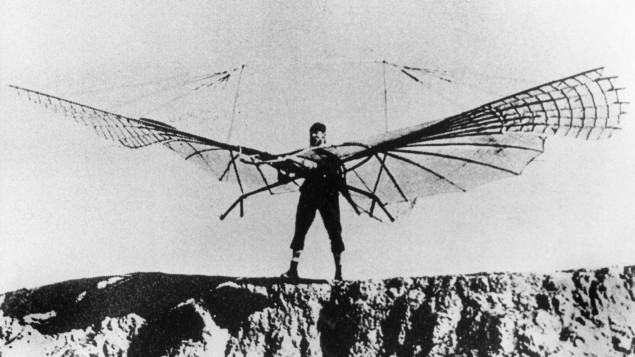
\includegraphics{otto_lilienthal}
    \caption{Otto Lilienthal with his flying apparatus. One example of how people failed in trying to imitate nature too closely. Source:\url{https://www.deutschlandfunkkultur.de/geschichte-der-fliegerei-wie-der-mensch-die-voegel.976.de.html?dram:article_id=308043}}
    \labfig{lilienthal}
\end{figure}

Warren McCulloch and Walter Pitts proposed one of the earliest models of an artificial neuron.
They aimed at simplifying models of a biological neuron at the time.
\marginnote{Notably McCulloch and Pitts (1943) even preceded Hodkin's and Huxley's (1952) Nobel price winning description of a neuron.}

\subsubsection{Biological Neuron}
For this reason, the functioning of a neuron shall be described shortly.

Human cells that make up the brain are called \textbf{neurons}.
They connected through dendrites, synapses, and axons.
These connections allow neurons to exchange signals with other neurons~\cite{grosse}.
This is a very simplified description, yet is gives a good how neurons work. 

A neuron receives signals through its dendrites, which all lead to the cell body (soma).
The cell body accumulates these signals.
If the summed value of the signals' potentials reaches a certain threshold, an action potential (spike) is generated.
The spike then travels as a signal along the axon and its branches towards other neurons.
\marginnote{Cell potentials are decreased by excitatory signals, as the action threshold sits below the resting potential.}
Axons end in synapses that connect to other neurons' dendrites.
Synaptic transmissions are usually mediated by chemicals and not by electrical signals.
The chemical nature of the synapse allows it to forward either an excitatory or an inhibitory signal.
Excitatory signals will bring the cell potential closer to the threshold, while inhibitory do the opposite~\cite[p.~42]{coloratlas}.

What makes the brain so powerful, though, is not the neuron itself with its arguably simple structure but the vast network of billions of these neurons.
Each neuron is connected to thousands of other neurons with which it communicates.
How a signal is transported between neurons depends on the interplay of synaptic weights, neural connections, and the threshold of each neuron.

\subsubsection{Artificial Neuron}
McCulloch and Pitts saw that powerful things could be achieved when connecting lots and lots of simple structures.
Thus, they proposed an even simpler model of a neuron: \\
They restricted their neuron to a binary state (on or off).
Each neuron gathers signals from other neurons, which are either positive or negative.
A neuron only becomes active if the number of incoming positive signals minus the number of negative signals exceeds the neuron's threshold.
\begin{marginfigure}
    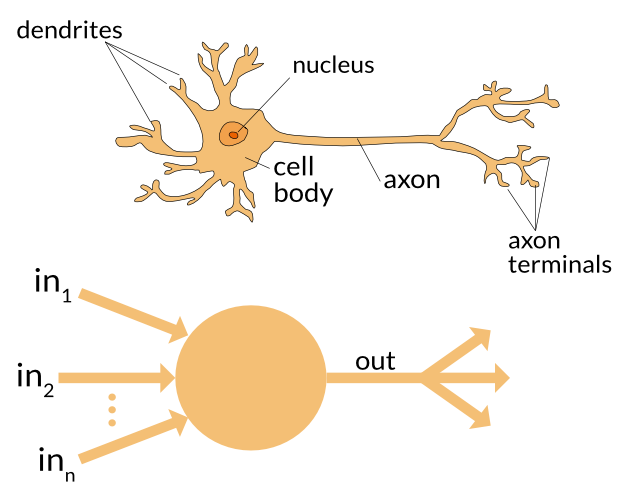
\includegraphics{neuron}
    \caption{Schematics of a neuron and a simple unit. Source:\url{https://appliedgo.net/media/perceptron/neuron.png}}
    \labfig{linear_class}
\end{marginfigure}
\begin{align}
    \labeq{mcculloch}
    g(x_1, x_2, ...) & = \sum_i^N x_i \\
    y = f(g(x_1, x_2, ...)) = \begin{cases} 1 \text{ if } g > 0 \\ 0 \text{else} \end{cases}
\end{align}
McCulloch and Pitts then also changed the highly parallel and complex nature of biological neural networks to a single layer feed-forward network architecture.

In a feed-forward network, neurons are grouped into layers and operate in parallel within a layer.
They do not interact within a layer.
Each neuron in a layer is fed the same input signal (often described as an input layer).
The neuron's state is then computed according to an equation such as \refeq{mcculloch}.
The activation value of each neuron then defines an output.

As this model deviates from nature quite a bit, these structures a better referred to as \textbf{units} instead of neurons.

In a single layer architecture, a layer often consists of a single unit (see \reffig{ff_arch}).
%\begin{marginfigure}
%    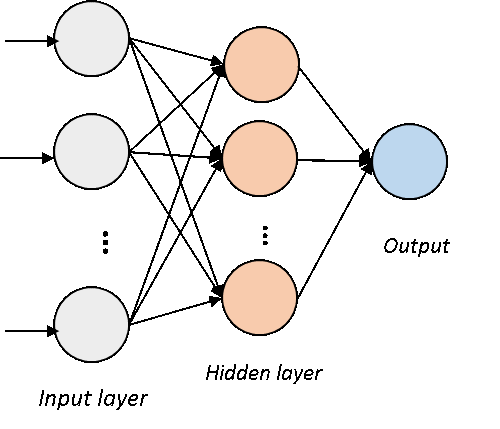
\includegraphics{feedforward}
%    \caption{Schmeatic of a feed-forward architecture.Source: \url{https://learning.oreilly.com/library/view/r-deep-learning/9781787121089/assets/32d89685-4e2b-4811-81e8-4654d0d98f91.png}}
%    \labfig{ff_arch}
%\end{marginfigure}
\begin{marginfigure}
    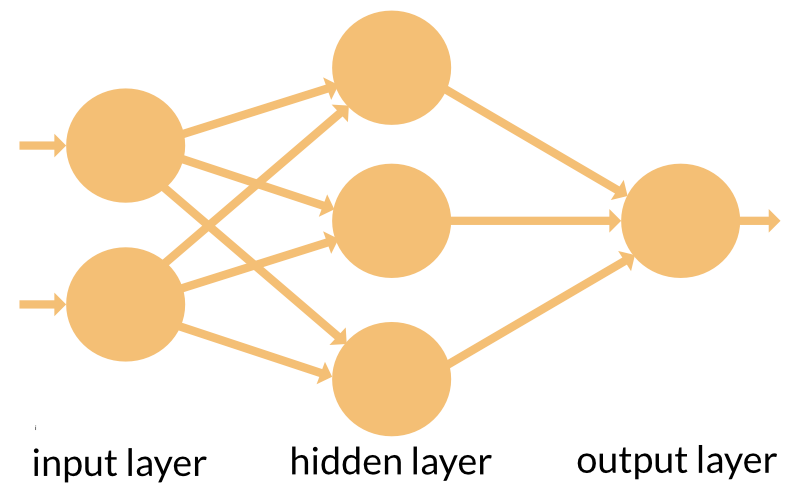
\includegraphics{ffnn}
    \caption{Schmeatic of a feed-forward architecture.Source:\url{https://appliedgo.net/media/perceptron/ffnn.png}}
    \labfig{ff_arch}
\end{marginfigure}
Basically, input signals come from one side, and output signals go out the other side, which can be expressed in a simple equation like \refeq{mcculloch}.
This is not only done for practical reasons but also inspired by the observation of layered neuron structures in the brain.

The McCulloch-Pitts model is capable of emulating simple logical relations (\lstinline|AND|, \lstinline|OR|, \lstinline|NOT|) but not \lstinline|XOR| which will be explained later.

\subsubsection{Perceptron}
As McCulloch's and Pitts' model is very much simplified yet comes with some weaknesses.
Thus, the \textbf{perceptron} has been introduced by Frank Rosenblatt in 1957.
Instead of having a binary unit, he came up with a linear threshold unit (LTU).
The LTU allows for numeric instead of binary signals, which can be weighted with independent factors.
Also, a unit's threshold/bias is parameterized as another weight with a constant input ($W_{i0} = 1$) using the ``bias trick''.
The resulting equation for each LTU then reads:
\begin{align}
    \labeq{LTU}
    a_i = \begin{cases}
        1 & \text{ if } \sum_{i=0}^n W_{ij} x_j \leq 0 \\
        -1 & \text{ if } \sum_{i=0}^n W_{ij} x_j > 0
    \end{cases}
\end{align}
Equation \refeq{LTU} can then be formulated in a vectorized form such that:
\begin{align}
    \labeq{perceptron}
    \vec{a} & = f(\mat{W}\vec{x}^T) \\
    f(x) & = \begin{cases} 1 & \text{ if } x \leq 0 \\  -1 & \text{ if } x > 0 \end{cases}
\end{align}

In this form, the calculations for each unit become mathematically and computationally relatively easy.
Each layer can be expressed as a vector of activations $\vec{x}$.
Multiplying this vector with the weight matrix $\mat{W}$ and applying the element-wise activation function returns the activations for the subsequent layer.\\
\marginnote{The word perceptron describes the whole function $f$ in \refeq{perceptron} which can consist of many LTUs}
%simplified computational model of how biological neurons might work together
This capable yet straightforward description of a unit built the base for the first surge of interest in neural networks (connectionism).

\subsubsection{Mathematical Interpretation}
The simplistic mathematical formulation of the perceptron suggests that there might be a mathematical meaning besides the biological analogy.
Indeed, the perceptron is equal to the definition of a \textbf{binary linear classifier}.

A binary linear classifier categorizes inputs into two classes, hence binary.
It does so by drawing a virtual hyperplane in input space and predicts the class for each input.
The decision depends on whether a point lies above or below this hyperplane.
\begin{marginfigure}
    \resizebox{\textwidth}{!}{
        %% Creator: Matplotlib, PGF backend
%%
%% To include the figure in your LaTeX document, write
%%   \input{<filename>.pgf}
%%
%% Make sure the required packages are loaded in your preamble
%%   \usepackage{pgf}
%%
%% and, on pdftex
%%   \usepackage[utf8]{inputenc}\DeclareUnicodeCharacter{2212}{-}
%%
%% or, on luatex and xetex
%%   \usepackage{unicode-math}
%%
%% Figures using additional raster images can only be included by \input if
%% they are in the same directory as the main LaTeX file. For loading figures
%% from other directories you can use the `import` package
%%   \usepackage{import}
%%
%% and then include the figures with
%%   \import{<path to file>}{<filename>.pgf}
%%
%% Matplotlib used the following preamble
%%
\begingroup%
\makeatletter%
\begin{pgfpicture}%
\pgfpathrectangle{\pgfpointorigin}{\pgfqpoint{10.000000in}{10.000000in}}%
\pgfusepath{use as bounding box, clip}%
\begin{pgfscope}%
\pgfsetbuttcap%
\pgfsetmiterjoin%
\definecolor{currentfill}{rgb}{1.000000,1.000000,1.000000}%
\pgfsetfillcolor{currentfill}%
\pgfsetlinewidth{0.000000pt}%
\definecolor{currentstroke}{rgb}{1.000000,1.000000,1.000000}%
\pgfsetstrokecolor{currentstroke}%
\pgfsetdash{}{0pt}%
\pgfpathmoveto{\pgfqpoint{0.000000in}{0.000000in}}%
\pgfpathlineto{\pgfqpoint{10.000000in}{0.000000in}}%
\pgfpathlineto{\pgfqpoint{10.000000in}{10.000000in}}%
\pgfpathlineto{\pgfqpoint{0.000000in}{10.000000in}}%
\pgfpathclose%
\pgfusepath{fill}%
\end{pgfscope}%
\begin{pgfscope}%
\pgfsetbuttcap%
\pgfsetmiterjoin%
\definecolor{currentfill}{rgb}{1.000000,1.000000,1.000000}%
\pgfsetfillcolor{currentfill}%
\pgfsetlinewidth{0.000000pt}%
\definecolor{currentstroke}{rgb}{0.000000,0.000000,0.000000}%
\pgfsetstrokecolor{currentstroke}%
\pgfsetstrokeopacity{0.000000}%
\pgfsetdash{}{0pt}%
\pgfpathmoveto{\pgfqpoint{1.250000in}{1.100000in}}%
\pgfpathlineto{\pgfqpoint{9.000000in}{1.100000in}}%
\pgfpathlineto{\pgfqpoint{9.000000in}{8.800000in}}%
\pgfpathlineto{\pgfqpoint{1.250000in}{8.800000in}}%
\pgfpathclose%
\pgfusepath{fill}%
\end{pgfscope}%
\begin{pgfscope}%
\pgfpathrectangle{\pgfqpoint{1.250000in}{1.100000in}}{\pgfqpoint{7.750000in}{7.700000in}}%
\pgfusepath{clip}%
\pgfsetbuttcap%
\pgfsetroundjoin%
\definecolor{currentfill}{rgb}{0.229806,0.298718,0.753683}%
\pgfsetfillcolor{currentfill}%
\pgfsetlinewidth{1.003750pt}%
\definecolor{currentstroke}{rgb}{0.229806,0.298718,0.753683}%
\pgfsetstrokecolor{currentstroke}%
\pgfsetdash{}{0pt}%
\pgfpathmoveto{\pgfqpoint{1.895833in}{1.700000in}}%
\pgfpathcurveto{\pgfqpoint{1.906883in}{1.700000in}}{\pgfqpoint{1.917482in}{1.704390in}}{\pgfqpoint{1.925296in}{1.712204in}}%
\pgfpathcurveto{\pgfqpoint{1.933110in}{1.720018in}}{\pgfqpoint{1.937500in}{1.730617in}}{\pgfqpoint{1.937500in}{1.741667in}}%
\pgfpathcurveto{\pgfqpoint{1.937500in}{1.752717in}}{\pgfqpoint{1.933110in}{1.763316in}}{\pgfqpoint{1.925296in}{1.771129in}}%
\pgfpathcurveto{\pgfqpoint{1.917482in}{1.778943in}}{\pgfqpoint{1.906883in}{1.783333in}}{\pgfqpoint{1.895833in}{1.783333in}}%
\pgfpathcurveto{\pgfqpoint{1.884783in}{1.783333in}}{\pgfqpoint{1.874184in}{1.778943in}}{\pgfqpoint{1.866371in}{1.771129in}}%
\pgfpathcurveto{\pgfqpoint{1.858557in}{1.763316in}}{\pgfqpoint{1.854167in}{1.752717in}}{\pgfqpoint{1.854167in}{1.741667in}}%
\pgfpathcurveto{\pgfqpoint{1.854167in}{1.730617in}}{\pgfqpoint{1.858557in}{1.720018in}}{\pgfqpoint{1.866371in}{1.712204in}}%
\pgfpathcurveto{\pgfqpoint{1.874184in}{1.704390in}}{\pgfqpoint{1.884783in}{1.700000in}}{\pgfqpoint{1.895833in}{1.700000in}}%
\pgfpathclose%
\pgfusepath{stroke,fill}%
\end{pgfscope}%
\begin{pgfscope}%
\pgfpathrectangle{\pgfqpoint{1.250000in}{1.100000in}}{\pgfqpoint{7.750000in}{7.700000in}}%
\pgfusepath{clip}%
\pgfsetbuttcap%
\pgfsetroundjoin%
\definecolor{currentfill}{rgb}{0.229806,0.298718,0.753683}%
\pgfsetfillcolor{currentfill}%
\pgfsetlinewidth{1.003750pt}%
\definecolor{currentstroke}{rgb}{0.229806,0.298718,0.753683}%
\pgfsetstrokecolor{currentstroke}%
\pgfsetdash{}{0pt}%
\pgfpathmoveto{\pgfqpoint{2.541667in}{4.266667in}}%
\pgfpathcurveto{\pgfqpoint{2.552717in}{4.266667in}}{\pgfqpoint{2.563316in}{4.271057in}}{\pgfqpoint{2.571129in}{4.278871in}}%
\pgfpathcurveto{\pgfqpoint{2.578943in}{4.286684in}}{\pgfqpoint{2.583333in}{4.297283in}}{\pgfqpoint{2.583333in}{4.308333in}}%
\pgfpathcurveto{\pgfqpoint{2.583333in}{4.319383in}}{\pgfqpoint{2.578943in}{4.329982in}}{\pgfqpoint{2.571129in}{4.337796in}}%
\pgfpathcurveto{\pgfqpoint{2.563316in}{4.345610in}}{\pgfqpoint{2.552717in}{4.350000in}}{\pgfqpoint{2.541667in}{4.350000in}}%
\pgfpathcurveto{\pgfqpoint{2.530617in}{4.350000in}}{\pgfqpoint{2.520018in}{4.345610in}}{\pgfqpoint{2.512204in}{4.337796in}}%
\pgfpathcurveto{\pgfqpoint{2.504390in}{4.329982in}}{\pgfqpoint{2.500000in}{4.319383in}}{\pgfqpoint{2.500000in}{4.308333in}}%
\pgfpathcurveto{\pgfqpoint{2.500000in}{4.297283in}}{\pgfqpoint{2.504390in}{4.286684in}}{\pgfqpoint{2.512204in}{4.278871in}}%
\pgfpathcurveto{\pgfqpoint{2.520018in}{4.271057in}}{\pgfqpoint{2.530617in}{4.266667in}}{\pgfqpoint{2.541667in}{4.266667in}}%
\pgfpathclose%
\pgfusepath{stroke,fill}%
\end{pgfscope}%
\begin{pgfscope}%
\pgfpathrectangle{\pgfqpoint{1.250000in}{1.100000in}}{\pgfqpoint{7.750000in}{7.700000in}}%
\pgfusepath{clip}%
\pgfsetbuttcap%
\pgfsetroundjoin%
\definecolor{currentfill}{rgb}{0.705673,0.015556,0.150233}%
\pgfsetfillcolor{currentfill}%
\pgfsetlinewidth{1.003750pt}%
\definecolor{currentstroke}{rgb}{0.705673,0.015556,0.150233}%
\pgfsetstrokecolor{currentstroke}%
\pgfsetdash{}{0pt}%
\pgfpathmoveto{\pgfqpoint{3.187500in}{6.833333in}}%
\pgfpathcurveto{\pgfqpoint{3.198550in}{6.833333in}}{\pgfqpoint{3.209149in}{6.837724in}}{\pgfqpoint{3.216963in}{6.845537in}}%
\pgfpathcurveto{\pgfqpoint{3.224776in}{6.853351in}}{\pgfqpoint{3.229167in}{6.863950in}}{\pgfqpoint{3.229167in}{6.875000in}}%
\pgfpathcurveto{\pgfqpoint{3.229167in}{6.886050in}}{\pgfqpoint{3.224776in}{6.896649in}}{\pgfqpoint{3.216963in}{6.904463in}}%
\pgfpathcurveto{\pgfqpoint{3.209149in}{6.912276in}}{\pgfqpoint{3.198550in}{6.916667in}}{\pgfqpoint{3.187500in}{6.916667in}}%
\pgfpathcurveto{\pgfqpoint{3.176450in}{6.916667in}}{\pgfqpoint{3.165851in}{6.912276in}}{\pgfqpoint{3.158037in}{6.904463in}}%
\pgfpathcurveto{\pgfqpoint{3.150224in}{6.896649in}}{\pgfqpoint{3.145833in}{6.886050in}}{\pgfqpoint{3.145833in}{6.875000in}}%
\pgfpathcurveto{\pgfqpoint{3.145833in}{6.863950in}}{\pgfqpoint{3.150224in}{6.853351in}}{\pgfqpoint{3.158037in}{6.845537in}}%
\pgfpathcurveto{\pgfqpoint{3.165851in}{6.837724in}}{\pgfqpoint{3.176450in}{6.833333in}}{\pgfqpoint{3.187500in}{6.833333in}}%
\pgfpathclose%
\pgfusepath{stroke,fill}%
\end{pgfscope}%
\begin{pgfscope}%
\pgfpathrectangle{\pgfqpoint{1.250000in}{1.100000in}}{\pgfqpoint{7.750000in}{7.700000in}}%
\pgfusepath{clip}%
\pgfsetbuttcap%
\pgfsetroundjoin%
\definecolor{currentfill}{rgb}{0.705673,0.015556,0.150233}%
\pgfsetfillcolor{currentfill}%
\pgfsetlinewidth{1.003750pt}%
\definecolor{currentstroke}{rgb}{0.705673,0.015556,0.150233}%
\pgfsetstrokecolor{currentstroke}%
\pgfsetdash{}{0pt}%
\pgfpathmoveto{\pgfqpoint{1.895833in}{6.191667in}}%
\pgfpathcurveto{\pgfqpoint{1.906883in}{6.191667in}}{\pgfqpoint{1.917482in}{6.196057in}}{\pgfqpoint{1.925296in}{6.203871in}}%
\pgfpathcurveto{\pgfqpoint{1.933110in}{6.211684in}}{\pgfqpoint{1.937500in}{6.222283in}}{\pgfqpoint{1.937500in}{6.233333in}}%
\pgfpathcurveto{\pgfqpoint{1.937500in}{6.244383in}}{\pgfqpoint{1.933110in}{6.254982in}}{\pgfqpoint{1.925296in}{6.262796in}}%
\pgfpathcurveto{\pgfqpoint{1.917482in}{6.270610in}}{\pgfqpoint{1.906883in}{6.275000in}}{\pgfqpoint{1.895833in}{6.275000in}}%
\pgfpathcurveto{\pgfqpoint{1.884783in}{6.275000in}}{\pgfqpoint{1.874184in}{6.270610in}}{\pgfqpoint{1.866371in}{6.262796in}}%
\pgfpathcurveto{\pgfqpoint{1.858557in}{6.254982in}}{\pgfqpoint{1.854167in}{6.244383in}}{\pgfqpoint{1.854167in}{6.233333in}}%
\pgfpathcurveto{\pgfqpoint{1.854167in}{6.222283in}}{\pgfqpoint{1.858557in}{6.211684in}}{\pgfqpoint{1.866371in}{6.203871in}}%
\pgfpathcurveto{\pgfqpoint{1.874184in}{6.196057in}}{\pgfqpoint{1.884783in}{6.191667in}}{\pgfqpoint{1.895833in}{6.191667in}}%
\pgfpathclose%
\pgfusepath{stroke,fill}%
\end{pgfscope}%
\begin{pgfscope}%
\pgfpathrectangle{\pgfqpoint{1.250000in}{1.100000in}}{\pgfqpoint{7.750000in}{7.700000in}}%
\pgfusepath{clip}%
\pgfsetbuttcap%
\pgfsetroundjoin%
\definecolor{currentfill}{rgb}{0.705673,0.015556,0.150233}%
\pgfsetfillcolor{currentfill}%
\pgfsetlinewidth{1.003750pt}%
\definecolor{currentstroke}{rgb}{0.705673,0.015556,0.150233}%
\pgfsetstrokecolor{currentstroke}%
\pgfsetdash{}{0pt}%
\pgfpathmoveto{\pgfqpoint{6.416667in}{6.191667in}}%
\pgfpathcurveto{\pgfqpoint{6.427717in}{6.191667in}}{\pgfqpoint{6.438316in}{6.196057in}}{\pgfqpoint{6.446129in}{6.203871in}}%
\pgfpathcurveto{\pgfqpoint{6.453943in}{6.211684in}}{\pgfqpoint{6.458333in}{6.222283in}}{\pgfqpoint{6.458333in}{6.233333in}}%
\pgfpathcurveto{\pgfqpoint{6.458333in}{6.244383in}}{\pgfqpoint{6.453943in}{6.254982in}}{\pgfqpoint{6.446129in}{6.262796in}}%
\pgfpathcurveto{\pgfqpoint{6.438316in}{6.270610in}}{\pgfqpoint{6.427717in}{6.275000in}}{\pgfqpoint{6.416667in}{6.275000in}}%
\pgfpathcurveto{\pgfqpoint{6.405617in}{6.275000in}}{\pgfqpoint{6.395018in}{6.270610in}}{\pgfqpoint{6.387204in}{6.262796in}}%
\pgfpathcurveto{\pgfqpoint{6.379390in}{6.254982in}}{\pgfqpoint{6.375000in}{6.244383in}}{\pgfqpoint{6.375000in}{6.233333in}}%
\pgfpathcurveto{\pgfqpoint{6.375000in}{6.222283in}}{\pgfqpoint{6.379390in}{6.211684in}}{\pgfqpoint{6.387204in}{6.203871in}}%
\pgfpathcurveto{\pgfqpoint{6.395018in}{6.196057in}}{\pgfqpoint{6.405617in}{6.191667in}}{\pgfqpoint{6.416667in}{6.191667in}}%
\pgfpathclose%
\pgfusepath{stroke,fill}%
\end{pgfscope}%
\begin{pgfscope}%
\pgfpathrectangle{\pgfqpoint{1.250000in}{1.100000in}}{\pgfqpoint{7.750000in}{7.700000in}}%
\pgfusepath{clip}%
\pgfsetbuttcap%
\pgfsetroundjoin%
\definecolor{currentfill}{rgb}{0.705673,0.015556,0.150233}%
\pgfsetfillcolor{currentfill}%
\pgfsetlinewidth{1.003750pt}%
\definecolor{currentstroke}{rgb}{0.705673,0.015556,0.150233}%
\pgfsetstrokecolor{currentstroke}%
\pgfsetdash{}{0pt}%
\pgfpathmoveto{\pgfqpoint{6.416667in}{6.833333in}}%
\pgfpathcurveto{\pgfqpoint{6.427717in}{6.833333in}}{\pgfqpoint{6.438316in}{6.837724in}}{\pgfqpoint{6.446129in}{6.845537in}}%
\pgfpathcurveto{\pgfqpoint{6.453943in}{6.853351in}}{\pgfqpoint{6.458333in}{6.863950in}}{\pgfqpoint{6.458333in}{6.875000in}}%
\pgfpathcurveto{\pgfqpoint{6.458333in}{6.886050in}}{\pgfqpoint{6.453943in}{6.896649in}}{\pgfqpoint{6.446129in}{6.904463in}}%
\pgfpathcurveto{\pgfqpoint{6.438316in}{6.912276in}}{\pgfqpoint{6.427717in}{6.916667in}}{\pgfqpoint{6.416667in}{6.916667in}}%
\pgfpathcurveto{\pgfqpoint{6.405617in}{6.916667in}}{\pgfqpoint{6.395018in}{6.912276in}}{\pgfqpoint{6.387204in}{6.904463in}}%
\pgfpathcurveto{\pgfqpoint{6.379390in}{6.896649in}}{\pgfqpoint{6.375000in}{6.886050in}}{\pgfqpoint{6.375000in}{6.875000in}}%
\pgfpathcurveto{\pgfqpoint{6.375000in}{6.863950in}}{\pgfqpoint{6.379390in}{6.853351in}}{\pgfqpoint{6.387204in}{6.845537in}}%
\pgfpathcurveto{\pgfqpoint{6.395018in}{6.837724in}}{\pgfqpoint{6.405617in}{6.833333in}}{\pgfqpoint{6.416667in}{6.833333in}}%
\pgfpathclose%
\pgfusepath{stroke,fill}%
\end{pgfscope}%
\begin{pgfscope}%
\pgfpathrectangle{\pgfqpoint{1.250000in}{1.100000in}}{\pgfqpoint{7.750000in}{7.700000in}}%
\pgfusepath{clip}%
\pgfsetbuttcap%
\pgfsetroundjoin%
\definecolor{currentfill}{rgb}{0.705673,0.015556,0.150233}%
\pgfsetfillcolor{currentfill}%
\pgfsetlinewidth{1.003750pt}%
\definecolor{currentstroke}{rgb}{0.705673,0.015556,0.150233}%
\pgfsetstrokecolor{currentstroke}%
\pgfsetdash{}{0pt}%
\pgfpathmoveto{\pgfqpoint{8.354167in}{2.983333in}}%
\pgfpathcurveto{\pgfqpoint{8.365217in}{2.983333in}}{\pgfqpoint{8.375816in}{2.987724in}}{\pgfqpoint{8.383629in}{2.995537in}}%
\pgfpathcurveto{\pgfqpoint{8.391443in}{3.003351in}}{\pgfqpoint{8.395833in}{3.013950in}}{\pgfqpoint{8.395833in}{3.025000in}}%
\pgfpathcurveto{\pgfqpoint{8.395833in}{3.036050in}}{\pgfqpoint{8.391443in}{3.046649in}}{\pgfqpoint{8.383629in}{3.054463in}}%
\pgfpathcurveto{\pgfqpoint{8.375816in}{3.062276in}}{\pgfqpoint{8.365217in}{3.066667in}}{\pgfqpoint{8.354167in}{3.066667in}}%
\pgfpathcurveto{\pgfqpoint{8.343117in}{3.066667in}}{\pgfqpoint{8.332518in}{3.062276in}}{\pgfqpoint{8.324704in}{3.054463in}}%
\pgfpathcurveto{\pgfqpoint{8.316890in}{3.046649in}}{\pgfqpoint{8.312500in}{3.036050in}}{\pgfqpoint{8.312500in}{3.025000in}}%
\pgfpathcurveto{\pgfqpoint{8.312500in}{3.013950in}}{\pgfqpoint{8.316890in}{3.003351in}}{\pgfqpoint{8.324704in}{2.995537in}}%
\pgfpathcurveto{\pgfqpoint{8.332518in}{2.987724in}}{\pgfqpoint{8.343117in}{2.983333in}}{\pgfqpoint{8.354167in}{2.983333in}}%
\pgfpathclose%
\pgfusepath{stroke,fill}%
\end{pgfscope}%
\begin{pgfscope}%
\pgfpathrectangle{\pgfqpoint{1.250000in}{1.100000in}}{\pgfqpoint{7.750000in}{7.700000in}}%
\pgfusepath{clip}%
\pgfsetbuttcap%
\pgfsetroundjoin%
\definecolor{currentfill}{rgb}{0.229806,0.298718,0.753683}%
\pgfsetfillcolor{currentfill}%
\pgfsetlinewidth{1.003750pt}%
\definecolor{currentstroke}{rgb}{0.229806,0.298718,0.753683}%
\pgfsetstrokecolor{currentstroke}%
\pgfsetdash{}{0pt}%
\pgfpathmoveto{\pgfqpoint{1.895833in}{2.341667in}}%
\pgfpathcurveto{\pgfqpoint{1.906883in}{2.341667in}}{\pgfqpoint{1.917482in}{2.346057in}}{\pgfqpoint{1.925296in}{2.353871in}}%
\pgfpathcurveto{\pgfqpoint{1.933110in}{2.361684in}}{\pgfqpoint{1.937500in}{2.372283in}}{\pgfqpoint{1.937500in}{2.383333in}}%
\pgfpathcurveto{\pgfqpoint{1.937500in}{2.394383in}}{\pgfqpoint{1.933110in}{2.404982in}}{\pgfqpoint{1.925296in}{2.412796in}}%
\pgfpathcurveto{\pgfqpoint{1.917482in}{2.420610in}}{\pgfqpoint{1.906883in}{2.425000in}}{\pgfqpoint{1.895833in}{2.425000in}}%
\pgfpathcurveto{\pgfqpoint{1.884783in}{2.425000in}}{\pgfqpoint{1.874184in}{2.420610in}}{\pgfqpoint{1.866371in}{2.412796in}}%
\pgfpathcurveto{\pgfqpoint{1.858557in}{2.404982in}}{\pgfqpoint{1.854167in}{2.394383in}}{\pgfqpoint{1.854167in}{2.383333in}}%
\pgfpathcurveto{\pgfqpoint{1.854167in}{2.372283in}}{\pgfqpoint{1.858557in}{2.361684in}}{\pgfqpoint{1.866371in}{2.353871in}}%
\pgfpathcurveto{\pgfqpoint{1.874184in}{2.346057in}}{\pgfqpoint{1.884783in}{2.341667in}}{\pgfqpoint{1.895833in}{2.341667in}}%
\pgfpathclose%
\pgfusepath{stroke,fill}%
\end{pgfscope}%
\begin{pgfscope}%
\pgfpathrectangle{\pgfqpoint{1.250000in}{1.100000in}}{\pgfqpoint{7.750000in}{7.700000in}}%
\pgfusepath{clip}%
\pgfsetbuttcap%
\pgfsetroundjoin%
\definecolor{currentfill}{rgb}{0.229806,0.298718,0.753683}%
\pgfsetfillcolor{currentfill}%
\pgfsetlinewidth{1.003750pt}%
\definecolor{currentstroke}{rgb}{0.229806,0.298718,0.753683}%
\pgfsetstrokecolor{currentstroke}%
\pgfsetdash{}{0pt}%
\pgfpathmoveto{\pgfqpoint{2.541667in}{2.341667in}}%
\pgfpathcurveto{\pgfqpoint{2.552717in}{2.341667in}}{\pgfqpoint{2.563316in}{2.346057in}}{\pgfqpoint{2.571129in}{2.353871in}}%
\pgfpathcurveto{\pgfqpoint{2.578943in}{2.361684in}}{\pgfqpoint{2.583333in}{2.372283in}}{\pgfqpoint{2.583333in}{2.383333in}}%
\pgfpathcurveto{\pgfqpoint{2.583333in}{2.394383in}}{\pgfqpoint{2.578943in}{2.404982in}}{\pgfqpoint{2.571129in}{2.412796in}}%
\pgfpathcurveto{\pgfqpoint{2.563316in}{2.420610in}}{\pgfqpoint{2.552717in}{2.425000in}}{\pgfqpoint{2.541667in}{2.425000in}}%
\pgfpathcurveto{\pgfqpoint{2.530617in}{2.425000in}}{\pgfqpoint{2.520018in}{2.420610in}}{\pgfqpoint{2.512204in}{2.412796in}}%
\pgfpathcurveto{\pgfqpoint{2.504390in}{2.404982in}}{\pgfqpoint{2.500000in}{2.394383in}}{\pgfqpoint{2.500000in}{2.383333in}}%
\pgfpathcurveto{\pgfqpoint{2.500000in}{2.372283in}}{\pgfqpoint{2.504390in}{2.361684in}}{\pgfqpoint{2.512204in}{2.353871in}}%
\pgfpathcurveto{\pgfqpoint{2.520018in}{2.346057in}}{\pgfqpoint{2.530617in}{2.341667in}}{\pgfqpoint{2.541667in}{2.341667in}}%
\pgfpathclose%
\pgfusepath{stroke,fill}%
\end{pgfscope}%
\begin{pgfscope}%
\pgfpathrectangle{\pgfqpoint{1.250000in}{1.100000in}}{\pgfqpoint{7.750000in}{7.700000in}}%
\pgfusepath{clip}%
\pgfsetbuttcap%
\pgfsetroundjoin%
\definecolor{currentfill}{rgb}{0.705673,0.015556,0.150233}%
\pgfsetfillcolor{currentfill}%
\pgfsetlinewidth{1.003750pt}%
\definecolor{currentstroke}{rgb}{0.705673,0.015556,0.150233}%
\pgfsetstrokecolor{currentstroke}%
\pgfsetdash{}{0pt}%
\pgfpathmoveto{\pgfqpoint{5.125000in}{4.908333in}}%
\pgfpathcurveto{\pgfqpoint{5.136050in}{4.908333in}}{\pgfqpoint{5.146649in}{4.912724in}}{\pgfqpoint{5.154463in}{4.920537in}}%
\pgfpathcurveto{\pgfqpoint{5.162276in}{4.928351in}}{\pgfqpoint{5.166667in}{4.938950in}}{\pgfqpoint{5.166667in}{4.950000in}}%
\pgfpathcurveto{\pgfqpoint{5.166667in}{4.961050in}}{\pgfqpoint{5.162276in}{4.971649in}}{\pgfqpoint{5.154463in}{4.979463in}}%
\pgfpathcurveto{\pgfqpoint{5.146649in}{4.987276in}}{\pgfqpoint{5.136050in}{4.991667in}}{\pgfqpoint{5.125000in}{4.991667in}}%
\pgfpathcurveto{\pgfqpoint{5.113950in}{4.991667in}}{\pgfqpoint{5.103351in}{4.987276in}}{\pgfqpoint{5.095537in}{4.979463in}}%
\pgfpathcurveto{\pgfqpoint{5.087724in}{4.971649in}}{\pgfqpoint{5.083333in}{4.961050in}}{\pgfqpoint{5.083333in}{4.950000in}}%
\pgfpathcurveto{\pgfqpoint{5.083333in}{4.938950in}}{\pgfqpoint{5.087724in}{4.928351in}}{\pgfqpoint{5.095537in}{4.920537in}}%
\pgfpathcurveto{\pgfqpoint{5.103351in}{4.912724in}}{\pgfqpoint{5.113950in}{4.908333in}}{\pgfqpoint{5.125000in}{4.908333in}}%
\pgfpathclose%
\pgfusepath{stroke,fill}%
\end{pgfscope}%
\begin{pgfscope}%
\pgfpathrectangle{\pgfqpoint{1.250000in}{1.100000in}}{\pgfqpoint{7.750000in}{7.700000in}}%
\pgfusepath{clip}%
\pgfsetbuttcap%
\pgfsetroundjoin%
\definecolor{currentfill}{rgb}{0.705673,0.015556,0.150233}%
\pgfsetfillcolor{currentfill}%
\pgfsetlinewidth{1.003750pt}%
\definecolor{currentstroke}{rgb}{0.705673,0.015556,0.150233}%
\pgfsetstrokecolor{currentstroke}%
\pgfsetdash{}{0pt}%
\pgfpathmoveto{\pgfqpoint{5.770833in}{4.908333in}}%
\pgfpathcurveto{\pgfqpoint{5.781883in}{4.908333in}}{\pgfqpoint{5.792482in}{4.912724in}}{\pgfqpoint{5.800296in}{4.920537in}}%
\pgfpathcurveto{\pgfqpoint{5.808110in}{4.928351in}}{\pgfqpoint{5.812500in}{4.938950in}}{\pgfqpoint{5.812500in}{4.950000in}}%
\pgfpathcurveto{\pgfqpoint{5.812500in}{4.961050in}}{\pgfqpoint{5.808110in}{4.971649in}}{\pgfqpoint{5.800296in}{4.979463in}}%
\pgfpathcurveto{\pgfqpoint{5.792482in}{4.987276in}}{\pgfqpoint{5.781883in}{4.991667in}}{\pgfqpoint{5.770833in}{4.991667in}}%
\pgfpathcurveto{\pgfqpoint{5.759783in}{4.991667in}}{\pgfqpoint{5.749184in}{4.987276in}}{\pgfqpoint{5.741371in}{4.979463in}}%
\pgfpathcurveto{\pgfqpoint{5.733557in}{4.971649in}}{\pgfqpoint{5.729167in}{4.961050in}}{\pgfqpoint{5.729167in}{4.950000in}}%
\pgfpathcurveto{\pgfqpoint{5.729167in}{4.938950in}}{\pgfqpoint{5.733557in}{4.928351in}}{\pgfqpoint{5.741371in}{4.920537in}}%
\pgfpathcurveto{\pgfqpoint{5.749184in}{4.912724in}}{\pgfqpoint{5.759783in}{4.908333in}}{\pgfqpoint{5.770833in}{4.908333in}}%
\pgfpathclose%
\pgfusepath{stroke,fill}%
\end{pgfscope}%
\begin{pgfscope}%
\pgfpathrectangle{\pgfqpoint{1.250000in}{1.100000in}}{\pgfqpoint{7.750000in}{7.700000in}}%
\pgfusepath{clip}%
\pgfsetbuttcap%
\pgfsetroundjoin%
\definecolor{currentfill}{rgb}{0.229806,0.298718,0.753683}%
\pgfsetfillcolor{currentfill}%
\pgfsetlinewidth{1.003750pt}%
\definecolor{currentstroke}{rgb}{0.229806,0.298718,0.753683}%
\pgfsetstrokecolor{currentstroke}%
\pgfsetdash{}{0pt}%
\pgfpathmoveto{\pgfqpoint{3.833333in}{2.341667in}}%
\pgfpathcurveto{\pgfqpoint{3.844383in}{2.341667in}}{\pgfqpoint{3.854982in}{2.346057in}}{\pgfqpoint{3.862796in}{2.353871in}}%
\pgfpathcurveto{\pgfqpoint{3.870610in}{2.361684in}}{\pgfqpoint{3.875000in}{2.372283in}}{\pgfqpoint{3.875000in}{2.383333in}}%
\pgfpathcurveto{\pgfqpoint{3.875000in}{2.394383in}}{\pgfqpoint{3.870610in}{2.404982in}}{\pgfqpoint{3.862796in}{2.412796in}}%
\pgfpathcurveto{\pgfqpoint{3.854982in}{2.420610in}}{\pgfqpoint{3.844383in}{2.425000in}}{\pgfqpoint{3.833333in}{2.425000in}}%
\pgfpathcurveto{\pgfqpoint{3.822283in}{2.425000in}}{\pgfqpoint{3.811684in}{2.420610in}}{\pgfqpoint{3.803871in}{2.412796in}}%
\pgfpathcurveto{\pgfqpoint{3.796057in}{2.404982in}}{\pgfqpoint{3.791667in}{2.394383in}}{\pgfqpoint{3.791667in}{2.383333in}}%
\pgfpathcurveto{\pgfqpoint{3.791667in}{2.372283in}}{\pgfqpoint{3.796057in}{2.361684in}}{\pgfqpoint{3.803871in}{2.353871in}}%
\pgfpathcurveto{\pgfqpoint{3.811684in}{2.346057in}}{\pgfqpoint{3.822283in}{2.341667in}}{\pgfqpoint{3.833333in}{2.341667in}}%
\pgfpathclose%
\pgfusepath{stroke,fill}%
\end{pgfscope}%
\begin{pgfscope}%
\pgfpathrectangle{\pgfqpoint{1.250000in}{1.100000in}}{\pgfqpoint{7.750000in}{7.700000in}}%
\pgfusepath{clip}%
\pgfsetbuttcap%
\pgfsetroundjoin%
\definecolor{currentfill}{rgb}{0.705673,0.015556,0.150233}%
\pgfsetfillcolor{currentfill}%
\pgfsetlinewidth{1.003750pt}%
\definecolor{currentstroke}{rgb}{0.705673,0.015556,0.150233}%
\pgfsetstrokecolor{currentstroke}%
\pgfsetdash{}{0pt}%
\pgfpathmoveto{\pgfqpoint{8.354167in}{8.116667in}}%
\pgfpathcurveto{\pgfqpoint{8.365217in}{8.116667in}}{\pgfqpoint{8.375816in}{8.121057in}}{\pgfqpoint{8.383629in}{8.128871in}}%
\pgfpathcurveto{\pgfqpoint{8.391443in}{8.136684in}}{\pgfqpoint{8.395833in}{8.147283in}}{\pgfqpoint{8.395833in}{8.158333in}}%
\pgfpathcurveto{\pgfqpoint{8.395833in}{8.169383in}}{\pgfqpoint{8.391443in}{8.179982in}}{\pgfqpoint{8.383629in}{8.187796in}}%
\pgfpathcurveto{\pgfqpoint{8.375816in}{8.195610in}}{\pgfqpoint{8.365217in}{8.200000in}}{\pgfqpoint{8.354167in}{8.200000in}}%
\pgfpathcurveto{\pgfqpoint{8.343117in}{8.200000in}}{\pgfqpoint{8.332518in}{8.195610in}}{\pgfqpoint{8.324704in}{8.187796in}}%
\pgfpathcurveto{\pgfqpoint{8.316890in}{8.179982in}}{\pgfqpoint{8.312500in}{8.169383in}}{\pgfqpoint{8.312500in}{8.158333in}}%
\pgfpathcurveto{\pgfqpoint{8.312500in}{8.147283in}}{\pgfqpoint{8.316890in}{8.136684in}}{\pgfqpoint{8.324704in}{8.128871in}}%
\pgfpathcurveto{\pgfqpoint{8.332518in}{8.121057in}}{\pgfqpoint{8.343117in}{8.116667in}}{\pgfqpoint{8.354167in}{8.116667in}}%
\pgfpathclose%
\pgfusepath{stroke,fill}%
\end{pgfscope}%
\begin{pgfscope}%
\pgfpathrectangle{\pgfqpoint{1.250000in}{1.100000in}}{\pgfqpoint{7.750000in}{7.700000in}}%
\pgfusepath{clip}%
\pgfsetbuttcap%
\pgfsetroundjoin%
\definecolor{currentfill}{rgb}{0.705673,0.015556,0.150233}%
\pgfsetfillcolor{currentfill}%
\pgfsetlinewidth{1.003750pt}%
\definecolor{currentstroke}{rgb}{0.705673,0.015556,0.150233}%
\pgfsetstrokecolor{currentstroke}%
\pgfsetdash{}{0pt}%
\pgfpathmoveto{\pgfqpoint{5.770833in}{3.625000in}}%
\pgfpathcurveto{\pgfqpoint{5.781883in}{3.625000in}}{\pgfqpoint{5.792482in}{3.629390in}}{\pgfqpoint{5.800296in}{3.637204in}}%
\pgfpathcurveto{\pgfqpoint{5.808110in}{3.645018in}}{\pgfqpoint{5.812500in}{3.655617in}}{\pgfqpoint{5.812500in}{3.666667in}}%
\pgfpathcurveto{\pgfqpoint{5.812500in}{3.677717in}}{\pgfqpoint{5.808110in}{3.688316in}}{\pgfqpoint{5.800296in}{3.696129in}}%
\pgfpathcurveto{\pgfqpoint{5.792482in}{3.703943in}}{\pgfqpoint{5.781883in}{3.708333in}}{\pgfqpoint{5.770833in}{3.708333in}}%
\pgfpathcurveto{\pgfqpoint{5.759783in}{3.708333in}}{\pgfqpoint{5.749184in}{3.703943in}}{\pgfqpoint{5.741371in}{3.696129in}}%
\pgfpathcurveto{\pgfqpoint{5.733557in}{3.688316in}}{\pgfqpoint{5.729167in}{3.677717in}}{\pgfqpoint{5.729167in}{3.666667in}}%
\pgfpathcurveto{\pgfqpoint{5.729167in}{3.655617in}}{\pgfqpoint{5.733557in}{3.645018in}}{\pgfqpoint{5.741371in}{3.637204in}}%
\pgfpathcurveto{\pgfqpoint{5.749184in}{3.629390in}}{\pgfqpoint{5.759783in}{3.625000in}}{\pgfqpoint{5.770833in}{3.625000in}}%
\pgfpathclose%
\pgfusepath{stroke,fill}%
\end{pgfscope}%
\begin{pgfscope}%
\pgfpathrectangle{\pgfqpoint{1.250000in}{1.100000in}}{\pgfqpoint{7.750000in}{7.700000in}}%
\pgfusepath{clip}%
\pgfsetbuttcap%
\pgfsetroundjoin%
\definecolor{currentfill}{rgb}{0.705673,0.015556,0.150233}%
\pgfsetfillcolor{currentfill}%
\pgfsetlinewidth{1.003750pt}%
\definecolor{currentstroke}{rgb}{0.705673,0.015556,0.150233}%
\pgfsetstrokecolor{currentstroke}%
\pgfsetdash{}{0pt}%
\pgfpathmoveto{\pgfqpoint{5.770833in}{5.550000in}}%
\pgfpathcurveto{\pgfqpoint{5.781883in}{5.550000in}}{\pgfqpoint{5.792482in}{5.554390in}}{\pgfqpoint{5.800296in}{5.562204in}}%
\pgfpathcurveto{\pgfqpoint{5.808110in}{5.570018in}}{\pgfqpoint{5.812500in}{5.580617in}}{\pgfqpoint{5.812500in}{5.591667in}}%
\pgfpathcurveto{\pgfqpoint{5.812500in}{5.602717in}}{\pgfqpoint{5.808110in}{5.613316in}}{\pgfqpoint{5.800296in}{5.621129in}}%
\pgfpathcurveto{\pgfqpoint{5.792482in}{5.628943in}}{\pgfqpoint{5.781883in}{5.633333in}}{\pgfqpoint{5.770833in}{5.633333in}}%
\pgfpathcurveto{\pgfqpoint{5.759783in}{5.633333in}}{\pgfqpoint{5.749184in}{5.628943in}}{\pgfqpoint{5.741371in}{5.621129in}}%
\pgfpathcurveto{\pgfqpoint{5.733557in}{5.613316in}}{\pgfqpoint{5.729167in}{5.602717in}}{\pgfqpoint{5.729167in}{5.591667in}}%
\pgfpathcurveto{\pgfqpoint{5.729167in}{5.580617in}}{\pgfqpoint{5.733557in}{5.570018in}}{\pgfqpoint{5.741371in}{5.562204in}}%
\pgfpathcurveto{\pgfqpoint{5.749184in}{5.554390in}}{\pgfqpoint{5.759783in}{5.550000in}}{\pgfqpoint{5.770833in}{5.550000in}}%
\pgfpathclose%
\pgfusepath{stroke,fill}%
\end{pgfscope}%
\begin{pgfscope}%
\pgfpathrectangle{\pgfqpoint{1.250000in}{1.100000in}}{\pgfqpoint{7.750000in}{7.700000in}}%
\pgfusepath{clip}%
\pgfsetbuttcap%
\pgfsetroundjoin%
\definecolor{currentfill}{rgb}{0.705673,0.015556,0.150233}%
\pgfsetfillcolor{currentfill}%
\pgfsetlinewidth{1.003750pt}%
\definecolor{currentstroke}{rgb}{0.705673,0.015556,0.150233}%
\pgfsetstrokecolor{currentstroke}%
\pgfsetdash{}{0pt}%
\pgfpathmoveto{\pgfqpoint{7.062500in}{1.700000in}}%
\pgfpathcurveto{\pgfqpoint{7.073550in}{1.700000in}}{\pgfqpoint{7.084149in}{1.704390in}}{\pgfqpoint{7.091963in}{1.712204in}}%
\pgfpathcurveto{\pgfqpoint{7.099776in}{1.720018in}}{\pgfqpoint{7.104167in}{1.730617in}}{\pgfqpoint{7.104167in}{1.741667in}}%
\pgfpathcurveto{\pgfqpoint{7.104167in}{1.752717in}}{\pgfqpoint{7.099776in}{1.763316in}}{\pgfqpoint{7.091963in}{1.771129in}}%
\pgfpathcurveto{\pgfqpoint{7.084149in}{1.778943in}}{\pgfqpoint{7.073550in}{1.783333in}}{\pgfqpoint{7.062500in}{1.783333in}}%
\pgfpathcurveto{\pgfqpoint{7.051450in}{1.783333in}}{\pgfqpoint{7.040851in}{1.778943in}}{\pgfqpoint{7.033037in}{1.771129in}}%
\pgfpathcurveto{\pgfqpoint{7.025224in}{1.763316in}}{\pgfqpoint{7.020833in}{1.752717in}}{\pgfqpoint{7.020833in}{1.741667in}}%
\pgfpathcurveto{\pgfqpoint{7.020833in}{1.730617in}}{\pgfqpoint{7.025224in}{1.720018in}}{\pgfqpoint{7.033037in}{1.712204in}}%
\pgfpathcurveto{\pgfqpoint{7.040851in}{1.704390in}}{\pgfqpoint{7.051450in}{1.700000in}}{\pgfqpoint{7.062500in}{1.700000in}}%
\pgfpathclose%
\pgfusepath{stroke,fill}%
\end{pgfscope}%
\begin{pgfscope}%
\pgfpathrectangle{\pgfqpoint{1.250000in}{1.100000in}}{\pgfqpoint{7.750000in}{7.700000in}}%
\pgfusepath{clip}%
\pgfsetbuttcap%
\pgfsetroundjoin%
\definecolor{currentfill}{rgb}{0.282910,0.105393,0.426902}%
\pgfsetfillcolor{currentfill}%
\pgfsetfillopacity{0.100000}%
\pgfsetlinewidth{0.000000pt}%
\definecolor{currentstroke}{rgb}{0.000000,0.000000,0.000000}%
\pgfsetstrokecolor{currentstroke}%
\pgfsetdash{}{0pt}%
\pgfpathmoveto{\pgfqpoint{1.328283in}{1.100000in}}%
\pgfpathlineto{\pgfqpoint{1.406566in}{1.100000in}}%
\pgfpathlineto{\pgfqpoint{1.484848in}{1.100000in}}%
\pgfpathlineto{\pgfqpoint{1.563131in}{1.100000in}}%
\pgfpathlineto{\pgfqpoint{1.641414in}{1.100000in}}%
\pgfpathlineto{\pgfqpoint{1.719697in}{1.100000in}}%
\pgfpathlineto{\pgfqpoint{1.797980in}{1.100000in}}%
\pgfpathlineto{\pgfqpoint{1.876263in}{1.100000in}}%
\pgfpathlineto{\pgfqpoint{1.954545in}{1.100000in}}%
\pgfpathlineto{\pgfqpoint{2.032828in}{1.100000in}}%
\pgfpathlineto{\pgfqpoint{2.111111in}{1.100000in}}%
\pgfpathlineto{\pgfqpoint{2.189394in}{1.100000in}}%
\pgfpathlineto{\pgfqpoint{2.267677in}{1.100000in}}%
\pgfpathlineto{\pgfqpoint{2.345960in}{1.100000in}}%
\pgfpathlineto{\pgfqpoint{2.424242in}{1.100000in}}%
\pgfpathlineto{\pgfqpoint{2.502525in}{1.100000in}}%
\pgfpathlineto{\pgfqpoint{2.580808in}{1.100000in}}%
\pgfpathlineto{\pgfqpoint{2.659091in}{1.100000in}}%
\pgfpathlineto{\pgfqpoint{2.737374in}{1.100000in}}%
\pgfpathlineto{\pgfqpoint{2.815657in}{1.100000in}}%
\pgfpathlineto{\pgfqpoint{2.893939in}{1.100000in}}%
\pgfpathlineto{\pgfqpoint{2.972222in}{1.100000in}}%
\pgfpathlineto{\pgfqpoint{3.050505in}{1.100000in}}%
\pgfpathlineto{\pgfqpoint{3.128788in}{1.100000in}}%
\pgfpathlineto{\pgfqpoint{3.207071in}{1.100000in}}%
\pgfpathlineto{\pgfqpoint{3.285354in}{1.100000in}}%
\pgfpathlineto{\pgfqpoint{3.363636in}{1.100000in}}%
\pgfpathlineto{\pgfqpoint{3.441919in}{1.100000in}}%
\pgfpathlineto{\pgfqpoint{3.520202in}{1.100000in}}%
\pgfpathlineto{\pgfqpoint{3.598485in}{1.100000in}}%
\pgfpathlineto{\pgfqpoint{3.676768in}{1.100000in}}%
\pgfpathlineto{\pgfqpoint{3.755051in}{1.100000in}}%
\pgfpathlineto{\pgfqpoint{3.833333in}{1.100000in}}%
\pgfpathlineto{\pgfqpoint{3.911616in}{1.100000in}}%
\pgfpathlineto{\pgfqpoint{3.989899in}{1.100000in}}%
\pgfpathlineto{\pgfqpoint{4.068182in}{1.100000in}}%
\pgfpathlineto{\pgfqpoint{4.146465in}{1.100000in}}%
\pgfpathlineto{\pgfqpoint{4.224747in}{1.100000in}}%
\pgfpathlineto{\pgfqpoint{4.303030in}{1.100000in}}%
\pgfpathlineto{\pgfqpoint{4.381313in}{1.100000in}}%
\pgfpathlineto{\pgfqpoint{4.459596in}{1.100000in}}%
\pgfpathlineto{\pgfqpoint{4.537879in}{1.100000in}}%
\pgfpathlineto{\pgfqpoint{4.616162in}{1.100000in}}%
\pgfpathlineto{\pgfqpoint{4.694444in}{1.100000in}}%
\pgfpathlineto{\pgfqpoint{4.772727in}{1.100000in}}%
\pgfpathlineto{\pgfqpoint{4.851010in}{1.100000in}}%
\pgfpathlineto{\pgfqpoint{4.929293in}{1.100000in}}%
\pgfpathlineto{\pgfqpoint{5.007576in}{1.100000in}}%
\pgfpathlineto{\pgfqpoint{5.085859in}{1.100000in}}%
\pgfpathlineto{\pgfqpoint{5.164141in}{1.100000in}}%
\pgfpathlineto{\pgfqpoint{5.242424in}{1.100000in}}%
\pgfpathlineto{\pgfqpoint{5.320707in}{1.100000in}}%
\pgfpathlineto{\pgfqpoint{5.398990in}{1.100000in}}%
\pgfpathlineto{\pgfqpoint{5.477273in}{1.100000in}}%
\pgfpathlineto{\pgfqpoint{5.555556in}{1.100000in}}%
\pgfpathlineto{\pgfqpoint{5.633838in}{1.100000in}}%
\pgfpathlineto{\pgfqpoint{5.712121in}{1.100000in}}%
\pgfpathlineto{\pgfqpoint{5.790404in}{1.100000in}}%
\pgfpathlineto{\pgfqpoint{5.868687in}{1.100000in}}%
\pgfpathlineto{\pgfqpoint{5.946970in}{1.100000in}}%
\pgfpathlineto{\pgfqpoint{6.025253in}{1.100000in}}%
\pgfpathlineto{\pgfqpoint{6.103535in}{1.100000in}}%
\pgfpathlineto{\pgfqpoint{6.181818in}{1.100000in}}%
\pgfpathlineto{\pgfqpoint{6.260101in}{1.100000in}}%
\pgfpathlineto{\pgfqpoint{6.338384in}{1.100000in}}%
\pgfpathlineto{\pgfqpoint{6.416667in}{1.100000in}}%
\pgfpathlineto{\pgfqpoint{6.428409in}{1.100000in}}%
\pgfpathlineto{\pgfqpoint{6.416667in}{1.111667in}}%
\pgfpathlineto{\pgfqpoint{6.350126in}{1.177778in}}%
\pgfpathlineto{\pgfqpoint{6.338384in}{1.189444in}}%
\pgfpathlineto{\pgfqpoint{6.271843in}{1.255556in}}%
\pgfpathlineto{\pgfqpoint{6.260101in}{1.267222in}}%
\pgfpathlineto{\pgfqpoint{6.193561in}{1.333333in}}%
\pgfpathlineto{\pgfqpoint{6.181818in}{1.345000in}}%
\pgfpathlineto{\pgfqpoint{6.115278in}{1.411111in}}%
\pgfpathlineto{\pgfqpoint{6.103535in}{1.422778in}}%
\pgfpathlineto{\pgfqpoint{6.025253in}{1.422778in}}%
\pgfpathlineto{\pgfqpoint{5.958712in}{1.488889in}}%
\pgfpathlineto{\pgfqpoint{5.946970in}{1.500556in}}%
\pgfpathlineto{\pgfqpoint{5.880429in}{1.566667in}}%
\pgfpathlineto{\pgfqpoint{5.880429in}{1.644444in}}%
\pgfpathlineto{\pgfqpoint{5.868687in}{1.656111in}}%
\pgfpathlineto{\pgfqpoint{5.802146in}{1.722222in}}%
\pgfpathlineto{\pgfqpoint{5.790404in}{1.733889in}}%
\pgfpathlineto{\pgfqpoint{5.723864in}{1.800000in}}%
\pgfpathlineto{\pgfqpoint{5.712121in}{1.811667in}}%
\pgfpathlineto{\pgfqpoint{5.645581in}{1.877778in}}%
\pgfpathlineto{\pgfqpoint{5.633838in}{1.889444in}}%
\pgfpathlineto{\pgfqpoint{5.567298in}{1.955556in}}%
\pgfpathlineto{\pgfqpoint{5.555556in}{1.967222in}}%
\pgfpathlineto{\pgfqpoint{5.489015in}{2.033333in}}%
\pgfpathlineto{\pgfqpoint{5.477273in}{2.045000in}}%
\pgfpathlineto{\pgfqpoint{5.410732in}{2.111111in}}%
\pgfpathlineto{\pgfqpoint{5.398990in}{2.122778in}}%
\pgfpathlineto{\pgfqpoint{5.332449in}{2.188889in}}%
\pgfpathlineto{\pgfqpoint{5.320707in}{2.200556in}}%
\pgfpathlineto{\pgfqpoint{5.254167in}{2.266667in}}%
\pgfpathlineto{\pgfqpoint{5.242424in}{2.278333in}}%
\pgfpathlineto{\pgfqpoint{5.175884in}{2.344444in}}%
\pgfpathlineto{\pgfqpoint{5.164141in}{2.356111in}}%
\pgfpathlineto{\pgfqpoint{5.097601in}{2.422222in}}%
\pgfpathlineto{\pgfqpoint{5.085859in}{2.433889in}}%
\pgfpathlineto{\pgfqpoint{5.019318in}{2.500000in}}%
\pgfpathlineto{\pgfqpoint{5.007576in}{2.511667in}}%
\pgfpathlineto{\pgfqpoint{4.941035in}{2.577778in}}%
\pgfpathlineto{\pgfqpoint{4.929293in}{2.589444in}}%
\pgfpathlineto{\pgfqpoint{4.862753in}{2.655556in}}%
\pgfpathlineto{\pgfqpoint{4.851010in}{2.667222in}}%
\pgfpathlineto{\pgfqpoint{4.784470in}{2.733333in}}%
\pgfpathlineto{\pgfqpoint{4.772727in}{2.745000in}}%
\pgfpathlineto{\pgfqpoint{4.694444in}{2.745000in}}%
\pgfpathlineto{\pgfqpoint{4.627904in}{2.811111in}}%
\pgfpathlineto{\pgfqpoint{4.627904in}{2.888889in}}%
\pgfpathlineto{\pgfqpoint{4.616162in}{2.900556in}}%
\pgfpathlineto{\pgfqpoint{4.549621in}{2.966667in}}%
\pgfpathlineto{\pgfqpoint{4.537879in}{2.978333in}}%
\pgfpathlineto{\pgfqpoint{4.471338in}{3.044444in}}%
\pgfpathlineto{\pgfqpoint{4.459596in}{3.056111in}}%
\pgfpathlineto{\pgfqpoint{4.393056in}{3.122222in}}%
\pgfpathlineto{\pgfqpoint{4.381313in}{3.133889in}}%
\pgfpathlineto{\pgfqpoint{4.314773in}{3.200000in}}%
\pgfpathlineto{\pgfqpoint{4.303030in}{3.211667in}}%
\pgfpathlineto{\pgfqpoint{4.236490in}{3.277778in}}%
\pgfpathlineto{\pgfqpoint{4.224747in}{3.289444in}}%
\pgfpathlineto{\pgfqpoint{4.158207in}{3.355556in}}%
\pgfpathlineto{\pgfqpoint{4.146465in}{3.367222in}}%
\pgfpathlineto{\pgfqpoint{4.079924in}{3.433333in}}%
\pgfpathlineto{\pgfqpoint{4.068182in}{3.445000in}}%
\pgfpathlineto{\pgfqpoint{4.001641in}{3.511111in}}%
\pgfpathlineto{\pgfqpoint{3.989899in}{3.522778in}}%
\pgfpathlineto{\pgfqpoint{3.923359in}{3.588889in}}%
\pgfpathlineto{\pgfqpoint{3.911616in}{3.600556in}}%
\pgfpathlineto{\pgfqpoint{3.845076in}{3.666667in}}%
\pgfpathlineto{\pgfqpoint{3.833333in}{3.678333in}}%
\pgfpathlineto{\pgfqpoint{3.766793in}{3.744444in}}%
\pgfpathlineto{\pgfqpoint{3.755051in}{3.756111in}}%
\pgfpathlineto{\pgfqpoint{3.688510in}{3.822222in}}%
\pgfpathlineto{\pgfqpoint{3.676768in}{3.833889in}}%
\pgfpathlineto{\pgfqpoint{3.610227in}{3.900000in}}%
\pgfpathlineto{\pgfqpoint{3.598485in}{3.911667in}}%
\pgfpathlineto{\pgfqpoint{3.531944in}{3.977778in}}%
\pgfpathlineto{\pgfqpoint{3.520202in}{3.989444in}}%
\pgfpathlineto{\pgfqpoint{3.453662in}{4.055556in}}%
\pgfpathlineto{\pgfqpoint{3.441919in}{4.067222in}}%
\pgfpathlineto{\pgfqpoint{3.375379in}{4.133333in}}%
\pgfpathlineto{\pgfqpoint{3.363636in}{4.145000in}}%
\pgfpathlineto{\pgfqpoint{3.297096in}{4.211111in}}%
\pgfpathlineto{\pgfqpoint{3.285354in}{4.222778in}}%
\pgfpathlineto{\pgfqpoint{3.218813in}{4.288889in}}%
\pgfpathlineto{\pgfqpoint{3.207071in}{4.300556in}}%
\pgfpathlineto{\pgfqpoint{3.140530in}{4.366667in}}%
\pgfpathlineto{\pgfqpoint{3.128788in}{4.378333in}}%
\pgfpathlineto{\pgfqpoint{3.062247in}{4.444444in}}%
\pgfpathlineto{\pgfqpoint{3.050505in}{4.456111in}}%
\pgfpathlineto{\pgfqpoint{2.972222in}{4.456111in}}%
\pgfpathlineto{\pgfqpoint{2.905682in}{4.522222in}}%
\pgfpathlineto{\pgfqpoint{2.905682in}{4.600000in}}%
\pgfpathlineto{\pgfqpoint{2.893939in}{4.611667in}}%
\pgfpathlineto{\pgfqpoint{2.827399in}{4.677778in}}%
\pgfpathlineto{\pgfqpoint{2.815657in}{4.689444in}}%
\pgfpathlineto{\pgfqpoint{2.749116in}{4.755556in}}%
\pgfpathlineto{\pgfqpoint{2.737374in}{4.767222in}}%
\pgfpathlineto{\pgfqpoint{2.670833in}{4.833333in}}%
\pgfpathlineto{\pgfqpoint{2.659091in}{4.845000in}}%
\pgfpathlineto{\pgfqpoint{2.592551in}{4.911111in}}%
\pgfpathlineto{\pgfqpoint{2.580808in}{4.922778in}}%
\pgfpathlineto{\pgfqpoint{2.514268in}{4.988889in}}%
\pgfpathlineto{\pgfqpoint{2.502525in}{5.000556in}}%
\pgfpathlineto{\pgfqpoint{2.435985in}{5.066667in}}%
\pgfpathlineto{\pgfqpoint{2.424242in}{5.078333in}}%
\pgfpathlineto{\pgfqpoint{2.357702in}{5.144444in}}%
\pgfpathlineto{\pgfqpoint{2.345960in}{5.156111in}}%
\pgfpathlineto{\pgfqpoint{2.279419in}{5.222222in}}%
\pgfpathlineto{\pgfqpoint{2.267677in}{5.233889in}}%
\pgfpathlineto{\pgfqpoint{2.201136in}{5.300000in}}%
\pgfpathlineto{\pgfqpoint{2.189394in}{5.311667in}}%
\pgfpathlineto{\pgfqpoint{2.122854in}{5.377778in}}%
\pgfpathlineto{\pgfqpoint{2.111111in}{5.389444in}}%
\pgfpathlineto{\pgfqpoint{2.044571in}{5.455556in}}%
\pgfpathlineto{\pgfqpoint{2.032828in}{5.467222in}}%
\pgfpathlineto{\pgfqpoint{1.966288in}{5.533333in}}%
\pgfpathlineto{\pgfqpoint{1.954545in}{5.545000in}}%
\pgfpathlineto{\pgfqpoint{1.888005in}{5.611111in}}%
\pgfpathlineto{\pgfqpoint{1.876263in}{5.622778in}}%
\pgfpathlineto{\pgfqpoint{1.809722in}{5.688889in}}%
\pgfpathlineto{\pgfqpoint{1.797980in}{5.700556in}}%
\pgfpathlineto{\pgfqpoint{1.719697in}{5.700556in}}%
\pgfpathlineto{\pgfqpoint{1.653157in}{5.766667in}}%
\pgfpathlineto{\pgfqpoint{1.641414in}{5.778333in}}%
\pgfpathlineto{\pgfqpoint{1.574874in}{5.844444in}}%
\pgfpathlineto{\pgfqpoint{1.574874in}{5.922222in}}%
\pgfpathlineto{\pgfqpoint{1.563131in}{5.933889in}}%
\pgfpathlineto{\pgfqpoint{1.496591in}{6.000000in}}%
\pgfpathlineto{\pgfqpoint{1.484848in}{6.011667in}}%
\pgfpathlineto{\pgfqpoint{1.418308in}{6.077778in}}%
\pgfpathlineto{\pgfqpoint{1.406566in}{6.089444in}}%
\pgfpathlineto{\pgfqpoint{1.340025in}{6.155556in}}%
\pgfpathlineto{\pgfqpoint{1.328283in}{6.167222in}}%
\pgfpathlineto{\pgfqpoint{1.261742in}{6.233333in}}%
\pgfpathlineto{\pgfqpoint{1.250000in}{6.245000in}}%
\pgfpathlineto{\pgfqpoint{1.250000in}{6.233333in}}%
\pgfpathlineto{\pgfqpoint{1.250000in}{6.155556in}}%
\pgfpathlineto{\pgfqpoint{1.250000in}{6.077778in}}%
\pgfpathlineto{\pgfqpoint{1.250000in}{6.000000in}}%
\pgfpathlineto{\pgfqpoint{1.250000in}{5.922222in}}%
\pgfpathlineto{\pgfqpoint{1.250000in}{5.844444in}}%
\pgfpathlineto{\pgfqpoint{1.250000in}{5.766667in}}%
\pgfpathlineto{\pgfqpoint{1.250000in}{5.688889in}}%
\pgfpathlineto{\pgfqpoint{1.250000in}{5.611111in}}%
\pgfpathlineto{\pgfqpoint{1.250000in}{5.533333in}}%
\pgfpathlineto{\pgfqpoint{1.250000in}{5.455556in}}%
\pgfpathlineto{\pgfqpoint{1.250000in}{5.377778in}}%
\pgfpathlineto{\pgfqpoint{1.250000in}{5.300000in}}%
\pgfpathlineto{\pgfqpoint{1.250000in}{5.222222in}}%
\pgfpathlineto{\pgfqpoint{1.250000in}{5.144444in}}%
\pgfpathlineto{\pgfqpoint{1.250000in}{5.066667in}}%
\pgfpathlineto{\pgfqpoint{1.250000in}{4.988889in}}%
\pgfpathlineto{\pgfqpoint{1.250000in}{4.911111in}}%
\pgfpathlineto{\pgfqpoint{1.250000in}{4.833333in}}%
\pgfpathlineto{\pgfqpoint{1.250000in}{4.755556in}}%
\pgfpathlineto{\pgfqpoint{1.250000in}{4.677778in}}%
\pgfpathlineto{\pgfqpoint{1.250000in}{4.600000in}}%
\pgfpathlineto{\pgfqpoint{1.250000in}{4.522222in}}%
\pgfpathlineto{\pgfqpoint{1.250000in}{4.444444in}}%
\pgfpathlineto{\pgfqpoint{1.250000in}{4.366667in}}%
\pgfpathlineto{\pgfqpoint{1.250000in}{4.288889in}}%
\pgfpathlineto{\pgfqpoint{1.250000in}{4.211111in}}%
\pgfpathlineto{\pgfqpoint{1.250000in}{4.133333in}}%
\pgfpathlineto{\pgfqpoint{1.250000in}{4.055556in}}%
\pgfpathlineto{\pgfqpoint{1.250000in}{3.977778in}}%
\pgfpathlineto{\pgfqpoint{1.250000in}{3.900000in}}%
\pgfpathlineto{\pgfqpoint{1.250000in}{3.822222in}}%
\pgfpathlineto{\pgfqpoint{1.250000in}{3.744444in}}%
\pgfpathlineto{\pgfqpoint{1.250000in}{3.666667in}}%
\pgfpathlineto{\pgfqpoint{1.250000in}{3.588889in}}%
\pgfpathlineto{\pgfqpoint{1.250000in}{3.511111in}}%
\pgfpathlineto{\pgfqpoint{1.250000in}{3.433333in}}%
\pgfpathlineto{\pgfqpoint{1.250000in}{3.355556in}}%
\pgfpathlineto{\pgfqpoint{1.250000in}{3.277778in}}%
\pgfpathlineto{\pgfqpoint{1.250000in}{3.200000in}}%
\pgfpathlineto{\pgfqpoint{1.250000in}{3.122222in}}%
\pgfpathlineto{\pgfqpoint{1.250000in}{3.044444in}}%
\pgfpathlineto{\pgfqpoint{1.250000in}{2.966667in}}%
\pgfpathlineto{\pgfqpoint{1.250000in}{2.888889in}}%
\pgfpathlineto{\pgfqpoint{1.250000in}{2.811111in}}%
\pgfpathlineto{\pgfqpoint{1.250000in}{2.733333in}}%
\pgfpathlineto{\pgfqpoint{1.250000in}{2.655556in}}%
\pgfpathlineto{\pgfqpoint{1.250000in}{2.577778in}}%
\pgfpathlineto{\pgfqpoint{1.250000in}{2.500000in}}%
\pgfpathlineto{\pgfqpoint{1.250000in}{2.422222in}}%
\pgfpathlineto{\pgfqpoint{1.250000in}{2.344444in}}%
\pgfpathlineto{\pgfqpoint{1.250000in}{2.266667in}}%
\pgfpathlineto{\pgfqpoint{1.250000in}{2.188889in}}%
\pgfpathlineto{\pgfqpoint{1.250000in}{2.111111in}}%
\pgfpathlineto{\pgfqpoint{1.250000in}{2.033333in}}%
\pgfpathlineto{\pgfqpoint{1.250000in}{1.955556in}}%
\pgfpathlineto{\pgfqpoint{1.250000in}{1.877778in}}%
\pgfpathlineto{\pgfqpoint{1.250000in}{1.800000in}}%
\pgfpathlineto{\pgfqpoint{1.250000in}{1.722222in}}%
\pgfpathlineto{\pgfqpoint{1.250000in}{1.644444in}}%
\pgfpathlineto{\pgfqpoint{1.250000in}{1.566667in}}%
\pgfpathlineto{\pgfqpoint{1.250000in}{1.488889in}}%
\pgfpathlineto{\pgfqpoint{1.250000in}{1.411111in}}%
\pgfpathlineto{\pgfqpoint{1.250000in}{1.333333in}}%
\pgfpathlineto{\pgfqpoint{1.250000in}{1.255556in}}%
\pgfpathlineto{\pgfqpoint{1.250000in}{1.177778in}}%
\pgfpathlineto{\pgfqpoint{1.250000in}{1.100000in}}%
\pgfpathclose%
\pgfusepath{fill}%
\end{pgfscope}%
\begin{pgfscope}%
\pgfpathrectangle{\pgfqpoint{1.250000in}{1.100000in}}{\pgfqpoint{7.750000in}{7.700000in}}%
\pgfusepath{clip}%
\pgfsetbuttcap%
\pgfsetroundjoin%
\definecolor{currentfill}{rgb}{0.248629,0.278775,0.534556}%
\pgfsetfillcolor{currentfill}%
\pgfsetfillopacity{0.100000}%
\pgfsetlinewidth{0.000000pt}%
\definecolor{currentstroke}{rgb}{0.000000,0.000000,0.000000}%
\pgfsetstrokecolor{currentstroke}%
\pgfsetdash{}{0pt}%
\pgfpathmoveto{\pgfqpoint{6.416667in}{1.111667in}}%
\pgfpathlineto{\pgfqpoint{6.428409in}{1.100000in}}%
\pgfpathlineto{\pgfqpoint{6.440152in}{1.100000in}}%
\pgfpathlineto{\pgfqpoint{6.416667in}{1.123333in}}%
\pgfpathlineto{\pgfqpoint{6.361869in}{1.177778in}}%
\pgfpathlineto{\pgfqpoint{6.338384in}{1.201111in}}%
\pgfpathlineto{\pgfqpoint{6.283586in}{1.255556in}}%
\pgfpathlineto{\pgfqpoint{6.260101in}{1.278889in}}%
\pgfpathlineto{\pgfqpoint{6.205303in}{1.333333in}}%
\pgfpathlineto{\pgfqpoint{6.181818in}{1.356667in}}%
\pgfpathlineto{\pgfqpoint{6.127020in}{1.411111in}}%
\pgfpathlineto{\pgfqpoint{6.103535in}{1.434444in}}%
\pgfpathlineto{\pgfqpoint{6.025253in}{1.434444in}}%
\pgfpathlineto{\pgfqpoint{5.970455in}{1.488889in}}%
\pgfpathlineto{\pgfqpoint{5.946970in}{1.512222in}}%
\pgfpathlineto{\pgfqpoint{5.892172in}{1.566667in}}%
\pgfpathlineto{\pgfqpoint{5.892172in}{1.644444in}}%
\pgfpathlineto{\pgfqpoint{5.868687in}{1.667778in}}%
\pgfpathlineto{\pgfqpoint{5.813889in}{1.722222in}}%
\pgfpathlineto{\pgfqpoint{5.790404in}{1.745556in}}%
\pgfpathlineto{\pgfqpoint{5.735606in}{1.800000in}}%
\pgfpathlineto{\pgfqpoint{5.712121in}{1.823333in}}%
\pgfpathlineto{\pgfqpoint{5.657323in}{1.877778in}}%
\pgfpathlineto{\pgfqpoint{5.633838in}{1.901111in}}%
\pgfpathlineto{\pgfqpoint{5.579040in}{1.955556in}}%
\pgfpathlineto{\pgfqpoint{5.555556in}{1.978889in}}%
\pgfpathlineto{\pgfqpoint{5.500758in}{2.033333in}}%
\pgfpathlineto{\pgfqpoint{5.477273in}{2.056667in}}%
\pgfpathlineto{\pgfqpoint{5.422475in}{2.111111in}}%
\pgfpathlineto{\pgfqpoint{5.398990in}{2.134444in}}%
\pgfpathlineto{\pgfqpoint{5.344192in}{2.188889in}}%
\pgfpathlineto{\pgfqpoint{5.320707in}{2.212222in}}%
\pgfpathlineto{\pgfqpoint{5.265909in}{2.266667in}}%
\pgfpathlineto{\pgfqpoint{5.242424in}{2.290000in}}%
\pgfpathlineto{\pgfqpoint{5.187626in}{2.344444in}}%
\pgfpathlineto{\pgfqpoint{5.164141in}{2.367778in}}%
\pgfpathlineto{\pgfqpoint{5.109343in}{2.422222in}}%
\pgfpathlineto{\pgfqpoint{5.085859in}{2.445556in}}%
\pgfpathlineto{\pgfqpoint{5.031061in}{2.500000in}}%
\pgfpathlineto{\pgfqpoint{5.007576in}{2.523333in}}%
\pgfpathlineto{\pgfqpoint{4.952778in}{2.577778in}}%
\pgfpathlineto{\pgfqpoint{4.929293in}{2.601111in}}%
\pgfpathlineto{\pgfqpoint{4.874495in}{2.655556in}}%
\pgfpathlineto{\pgfqpoint{4.851010in}{2.678889in}}%
\pgfpathlineto{\pgfqpoint{4.796212in}{2.733333in}}%
\pgfpathlineto{\pgfqpoint{4.772727in}{2.756667in}}%
\pgfpathlineto{\pgfqpoint{4.694444in}{2.756667in}}%
\pgfpathlineto{\pgfqpoint{4.639646in}{2.811111in}}%
\pgfpathlineto{\pgfqpoint{4.639646in}{2.888889in}}%
\pgfpathlineto{\pgfqpoint{4.616162in}{2.912222in}}%
\pgfpathlineto{\pgfqpoint{4.561364in}{2.966667in}}%
\pgfpathlineto{\pgfqpoint{4.537879in}{2.990000in}}%
\pgfpathlineto{\pgfqpoint{4.483081in}{3.044444in}}%
\pgfpathlineto{\pgfqpoint{4.459596in}{3.067778in}}%
\pgfpathlineto{\pgfqpoint{4.404798in}{3.122222in}}%
\pgfpathlineto{\pgfqpoint{4.381313in}{3.145556in}}%
\pgfpathlineto{\pgfqpoint{4.326515in}{3.200000in}}%
\pgfpathlineto{\pgfqpoint{4.303030in}{3.223333in}}%
\pgfpathlineto{\pgfqpoint{4.248232in}{3.277778in}}%
\pgfpathlineto{\pgfqpoint{4.224747in}{3.301111in}}%
\pgfpathlineto{\pgfqpoint{4.169949in}{3.355556in}}%
\pgfpathlineto{\pgfqpoint{4.146465in}{3.378889in}}%
\pgfpathlineto{\pgfqpoint{4.091667in}{3.433333in}}%
\pgfpathlineto{\pgfqpoint{4.068182in}{3.456667in}}%
\pgfpathlineto{\pgfqpoint{4.013384in}{3.511111in}}%
\pgfpathlineto{\pgfqpoint{3.989899in}{3.534444in}}%
\pgfpathlineto{\pgfqpoint{3.935101in}{3.588889in}}%
\pgfpathlineto{\pgfqpoint{3.911616in}{3.612222in}}%
\pgfpathlineto{\pgfqpoint{3.856818in}{3.666667in}}%
\pgfpathlineto{\pgfqpoint{3.833333in}{3.690000in}}%
\pgfpathlineto{\pgfqpoint{3.778535in}{3.744444in}}%
\pgfpathlineto{\pgfqpoint{3.755051in}{3.767778in}}%
\pgfpathlineto{\pgfqpoint{3.700253in}{3.822222in}}%
\pgfpathlineto{\pgfqpoint{3.676768in}{3.845556in}}%
\pgfpathlineto{\pgfqpoint{3.621970in}{3.900000in}}%
\pgfpathlineto{\pgfqpoint{3.598485in}{3.923333in}}%
\pgfpathlineto{\pgfqpoint{3.543687in}{3.977778in}}%
\pgfpathlineto{\pgfqpoint{3.520202in}{4.001111in}}%
\pgfpathlineto{\pgfqpoint{3.465404in}{4.055556in}}%
\pgfpathlineto{\pgfqpoint{3.441919in}{4.078889in}}%
\pgfpathlineto{\pgfqpoint{3.387121in}{4.133333in}}%
\pgfpathlineto{\pgfqpoint{3.363636in}{4.156667in}}%
\pgfpathlineto{\pgfqpoint{3.308838in}{4.211111in}}%
\pgfpathlineto{\pgfqpoint{3.285354in}{4.234444in}}%
\pgfpathlineto{\pgfqpoint{3.230556in}{4.288889in}}%
\pgfpathlineto{\pgfqpoint{3.207071in}{4.312222in}}%
\pgfpathlineto{\pgfqpoint{3.152273in}{4.366667in}}%
\pgfpathlineto{\pgfqpoint{3.128788in}{4.390000in}}%
\pgfpathlineto{\pgfqpoint{3.073990in}{4.444444in}}%
\pgfpathlineto{\pgfqpoint{3.050505in}{4.467778in}}%
\pgfpathlineto{\pgfqpoint{2.972222in}{4.467778in}}%
\pgfpathlineto{\pgfqpoint{2.917424in}{4.522222in}}%
\pgfpathlineto{\pgfqpoint{2.917424in}{4.600000in}}%
\pgfpathlineto{\pgfqpoint{2.893939in}{4.623333in}}%
\pgfpathlineto{\pgfqpoint{2.839141in}{4.677778in}}%
\pgfpathlineto{\pgfqpoint{2.815657in}{4.701111in}}%
\pgfpathlineto{\pgfqpoint{2.760859in}{4.755556in}}%
\pgfpathlineto{\pgfqpoint{2.737374in}{4.778889in}}%
\pgfpathlineto{\pgfqpoint{2.682576in}{4.833333in}}%
\pgfpathlineto{\pgfqpoint{2.659091in}{4.856667in}}%
\pgfpathlineto{\pgfqpoint{2.604293in}{4.911111in}}%
\pgfpathlineto{\pgfqpoint{2.580808in}{4.934444in}}%
\pgfpathlineto{\pgfqpoint{2.526010in}{4.988889in}}%
\pgfpathlineto{\pgfqpoint{2.502525in}{5.012222in}}%
\pgfpathlineto{\pgfqpoint{2.447727in}{5.066667in}}%
\pgfpathlineto{\pgfqpoint{2.424242in}{5.090000in}}%
\pgfpathlineto{\pgfqpoint{2.369444in}{5.144444in}}%
\pgfpathlineto{\pgfqpoint{2.345960in}{5.167778in}}%
\pgfpathlineto{\pgfqpoint{2.291162in}{5.222222in}}%
\pgfpathlineto{\pgfqpoint{2.267677in}{5.245556in}}%
\pgfpathlineto{\pgfqpoint{2.212879in}{5.300000in}}%
\pgfpathlineto{\pgfqpoint{2.189394in}{5.323333in}}%
\pgfpathlineto{\pgfqpoint{2.134596in}{5.377778in}}%
\pgfpathlineto{\pgfqpoint{2.111111in}{5.401111in}}%
\pgfpathlineto{\pgfqpoint{2.056313in}{5.455556in}}%
\pgfpathlineto{\pgfqpoint{2.032828in}{5.478889in}}%
\pgfpathlineto{\pgfqpoint{1.978030in}{5.533333in}}%
\pgfpathlineto{\pgfqpoint{1.954545in}{5.556667in}}%
\pgfpathlineto{\pgfqpoint{1.899747in}{5.611111in}}%
\pgfpathlineto{\pgfqpoint{1.876263in}{5.634444in}}%
\pgfpathlineto{\pgfqpoint{1.821465in}{5.688889in}}%
\pgfpathlineto{\pgfqpoint{1.797980in}{5.712222in}}%
\pgfpathlineto{\pgfqpoint{1.719697in}{5.712222in}}%
\pgfpathlineto{\pgfqpoint{1.664899in}{5.766667in}}%
\pgfpathlineto{\pgfqpoint{1.641414in}{5.790000in}}%
\pgfpathlineto{\pgfqpoint{1.586616in}{5.844444in}}%
\pgfpathlineto{\pgfqpoint{1.586616in}{5.922222in}}%
\pgfpathlineto{\pgfqpoint{1.563131in}{5.945556in}}%
\pgfpathlineto{\pgfqpoint{1.508333in}{6.000000in}}%
\pgfpathlineto{\pgfqpoint{1.484848in}{6.023333in}}%
\pgfpathlineto{\pgfqpoint{1.430051in}{6.077778in}}%
\pgfpathlineto{\pgfqpoint{1.406566in}{6.101111in}}%
\pgfpathlineto{\pgfqpoint{1.351768in}{6.155556in}}%
\pgfpathlineto{\pgfqpoint{1.328283in}{6.178889in}}%
\pgfpathlineto{\pgfqpoint{1.273485in}{6.233333in}}%
\pgfpathlineto{\pgfqpoint{1.250000in}{6.256667in}}%
\pgfpathlineto{\pgfqpoint{1.250000in}{6.245000in}}%
\pgfpathlineto{\pgfqpoint{1.261742in}{6.233333in}}%
\pgfpathlineto{\pgfqpoint{1.328283in}{6.167222in}}%
\pgfpathlineto{\pgfqpoint{1.340025in}{6.155556in}}%
\pgfpathlineto{\pgfqpoint{1.406566in}{6.089444in}}%
\pgfpathlineto{\pgfqpoint{1.418308in}{6.077778in}}%
\pgfpathlineto{\pgfqpoint{1.484848in}{6.011667in}}%
\pgfpathlineto{\pgfqpoint{1.496591in}{6.000000in}}%
\pgfpathlineto{\pgfqpoint{1.563131in}{5.933889in}}%
\pgfpathlineto{\pgfqpoint{1.574874in}{5.922222in}}%
\pgfpathlineto{\pgfqpoint{1.574874in}{5.844444in}}%
\pgfpathlineto{\pgfqpoint{1.641414in}{5.778333in}}%
\pgfpathlineto{\pgfqpoint{1.653157in}{5.766667in}}%
\pgfpathlineto{\pgfqpoint{1.719697in}{5.700556in}}%
\pgfpathlineto{\pgfqpoint{1.797980in}{5.700556in}}%
\pgfpathlineto{\pgfqpoint{1.809722in}{5.688889in}}%
\pgfpathlineto{\pgfqpoint{1.876263in}{5.622778in}}%
\pgfpathlineto{\pgfqpoint{1.888005in}{5.611111in}}%
\pgfpathlineto{\pgfqpoint{1.954545in}{5.545000in}}%
\pgfpathlineto{\pgfqpoint{1.966288in}{5.533333in}}%
\pgfpathlineto{\pgfqpoint{2.032828in}{5.467222in}}%
\pgfpathlineto{\pgfqpoint{2.044571in}{5.455556in}}%
\pgfpathlineto{\pgfqpoint{2.111111in}{5.389444in}}%
\pgfpathlineto{\pgfqpoint{2.122854in}{5.377778in}}%
\pgfpathlineto{\pgfqpoint{2.189394in}{5.311667in}}%
\pgfpathlineto{\pgfqpoint{2.201136in}{5.300000in}}%
\pgfpathlineto{\pgfqpoint{2.267677in}{5.233889in}}%
\pgfpathlineto{\pgfqpoint{2.279419in}{5.222222in}}%
\pgfpathlineto{\pgfqpoint{2.345960in}{5.156111in}}%
\pgfpathlineto{\pgfqpoint{2.357702in}{5.144444in}}%
\pgfpathlineto{\pgfqpoint{2.424242in}{5.078333in}}%
\pgfpathlineto{\pgfqpoint{2.435985in}{5.066667in}}%
\pgfpathlineto{\pgfqpoint{2.502525in}{5.000556in}}%
\pgfpathlineto{\pgfqpoint{2.514268in}{4.988889in}}%
\pgfpathlineto{\pgfqpoint{2.580808in}{4.922778in}}%
\pgfpathlineto{\pgfqpoint{2.592551in}{4.911111in}}%
\pgfpathlineto{\pgfqpoint{2.659091in}{4.845000in}}%
\pgfpathlineto{\pgfqpoint{2.670833in}{4.833333in}}%
\pgfpathlineto{\pgfqpoint{2.737374in}{4.767222in}}%
\pgfpathlineto{\pgfqpoint{2.749116in}{4.755556in}}%
\pgfpathlineto{\pgfqpoint{2.815657in}{4.689444in}}%
\pgfpathlineto{\pgfqpoint{2.827399in}{4.677778in}}%
\pgfpathlineto{\pgfqpoint{2.893939in}{4.611667in}}%
\pgfpathlineto{\pgfqpoint{2.905682in}{4.600000in}}%
\pgfpathlineto{\pgfqpoint{2.905682in}{4.522222in}}%
\pgfpathlineto{\pgfqpoint{2.972222in}{4.456111in}}%
\pgfpathlineto{\pgfqpoint{3.050505in}{4.456111in}}%
\pgfpathlineto{\pgfqpoint{3.062247in}{4.444444in}}%
\pgfpathlineto{\pgfqpoint{3.128788in}{4.378333in}}%
\pgfpathlineto{\pgfqpoint{3.140530in}{4.366667in}}%
\pgfpathlineto{\pgfqpoint{3.207071in}{4.300556in}}%
\pgfpathlineto{\pgfqpoint{3.218813in}{4.288889in}}%
\pgfpathlineto{\pgfqpoint{3.285354in}{4.222778in}}%
\pgfpathlineto{\pgfqpoint{3.297096in}{4.211111in}}%
\pgfpathlineto{\pgfqpoint{3.363636in}{4.145000in}}%
\pgfpathlineto{\pgfqpoint{3.375379in}{4.133333in}}%
\pgfpathlineto{\pgfqpoint{3.441919in}{4.067222in}}%
\pgfpathlineto{\pgfqpoint{3.453662in}{4.055556in}}%
\pgfpathlineto{\pgfqpoint{3.520202in}{3.989444in}}%
\pgfpathlineto{\pgfqpoint{3.531944in}{3.977778in}}%
\pgfpathlineto{\pgfqpoint{3.598485in}{3.911667in}}%
\pgfpathlineto{\pgfqpoint{3.610227in}{3.900000in}}%
\pgfpathlineto{\pgfqpoint{3.676768in}{3.833889in}}%
\pgfpathlineto{\pgfqpoint{3.688510in}{3.822222in}}%
\pgfpathlineto{\pgfqpoint{3.755051in}{3.756111in}}%
\pgfpathlineto{\pgfqpoint{3.766793in}{3.744444in}}%
\pgfpathlineto{\pgfqpoint{3.833333in}{3.678333in}}%
\pgfpathlineto{\pgfqpoint{3.845076in}{3.666667in}}%
\pgfpathlineto{\pgfqpoint{3.911616in}{3.600556in}}%
\pgfpathlineto{\pgfqpoint{3.923359in}{3.588889in}}%
\pgfpathlineto{\pgfqpoint{3.989899in}{3.522778in}}%
\pgfpathlineto{\pgfqpoint{4.001641in}{3.511111in}}%
\pgfpathlineto{\pgfqpoint{4.068182in}{3.445000in}}%
\pgfpathlineto{\pgfqpoint{4.079924in}{3.433333in}}%
\pgfpathlineto{\pgfqpoint{4.146465in}{3.367222in}}%
\pgfpathlineto{\pgfqpoint{4.158207in}{3.355556in}}%
\pgfpathlineto{\pgfqpoint{4.224747in}{3.289444in}}%
\pgfpathlineto{\pgfqpoint{4.236490in}{3.277778in}}%
\pgfpathlineto{\pgfqpoint{4.303030in}{3.211667in}}%
\pgfpathlineto{\pgfqpoint{4.314773in}{3.200000in}}%
\pgfpathlineto{\pgfqpoint{4.381313in}{3.133889in}}%
\pgfpathlineto{\pgfqpoint{4.393056in}{3.122222in}}%
\pgfpathlineto{\pgfqpoint{4.459596in}{3.056111in}}%
\pgfpathlineto{\pgfqpoint{4.471338in}{3.044444in}}%
\pgfpathlineto{\pgfqpoint{4.537879in}{2.978333in}}%
\pgfpathlineto{\pgfqpoint{4.549621in}{2.966667in}}%
\pgfpathlineto{\pgfqpoint{4.616162in}{2.900556in}}%
\pgfpathlineto{\pgfqpoint{4.627904in}{2.888889in}}%
\pgfpathlineto{\pgfqpoint{4.627904in}{2.811111in}}%
\pgfpathlineto{\pgfqpoint{4.694444in}{2.745000in}}%
\pgfpathlineto{\pgfqpoint{4.772727in}{2.745000in}}%
\pgfpathlineto{\pgfqpoint{4.784470in}{2.733333in}}%
\pgfpathlineto{\pgfqpoint{4.851010in}{2.667222in}}%
\pgfpathlineto{\pgfqpoint{4.862753in}{2.655556in}}%
\pgfpathlineto{\pgfqpoint{4.929293in}{2.589444in}}%
\pgfpathlineto{\pgfqpoint{4.941035in}{2.577778in}}%
\pgfpathlineto{\pgfqpoint{5.007576in}{2.511667in}}%
\pgfpathlineto{\pgfqpoint{5.019318in}{2.500000in}}%
\pgfpathlineto{\pgfqpoint{5.085859in}{2.433889in}}%
\pgfpathlineto{\pgfqpoint{5.097601in}{2.422222in}}%
\pgfpathlineto{\pgfqpoint{5.164141in}{2.356111in}}%
\pgfpathlineto{\pgfqpoint{5.175884in}{2.344444in}}%
\pgfpathlineto{\pgfqpoint{5.242424in}{2.278333in}}%
\pgfpathlineto{\pgfqpoint{5.254167in}{2.266667in}}%
\pgfpathlineto{\pgfqpoint{5.320707in}{2.200556in}}%
\pgfpathlineto{\pgfqpoint{5.332449in}{2.188889in}}%
\pgfpathlineto{\pgfqpoint{5.398990in}{2.122778in}}%
\pgfpathlineto{\pgfqpoint{5.410732in}{2.111111in}}%
\pgfpathlineto{\pgfqpoint{5.477273in}{2.045000in}}%
\pgfpathlineto{\pgfqpoint{5.489015in}{2.033333in}}%
\pgfpathlineto{\pgfqpoint{5.555556in}{1.967222in}}%
\pgfpathlineto{\pgfqpoint{5.567298in}{1.955556in}}%
\pgfpathlineto{\pgfqpoint{5.633838in}{1.889444in}}%
\pgfpathlineto{\pgfqpoint{5.645581in}{1.877778in}}%
\pgfpathlineto{\pgfqpoint{5.712121in}{1.811667in}}%
\pgfpathlineto{\pgfqpoint{5.723864in}{1.800000in}}%
\pgfpathlineto{\pgfqpoint{5.790404in}{1.733889in}}%
\pgfpathlineto{\pgfqpoint{5.802146in}{1.722222in}}%
\pgfpathlineto{\pgfqpoint{5.868687in}{1.656111in}}%
\pgfpathlineto{\pgfqpoint{5.880429in}{1.644444in}}%
\pgfpathlineto{\pgfqpoint{5.880429in}{1.566667in}}%
\pgfpathlineto{\pgfqpoint{5.946970in}{1.500556in}}%
\pgfpathlineto{\pgfqpoint{5.958712in}{1.488889in}}%
\pgfpathlineto{\pgfqpoint{6.025253in}{1.422778in}}%
\pgfpathlineto{\pgfqpoint{6.103535in}{1.422778in}}%
\pgfpathlineto{\pgfqpoint{6.115278in}{1.411111in}}%
\pgfpathlineto{\pgfqpoint{6.181818in}{1.345000in}}%
\pgfpathlineto{\pgfqpoint{6.193561in}{1.333333in}}%
\pgfpathlineto{\pgfqpoint{6.260101in}{1.267222in}}%
\pgfpathlineto{\pgfqpoint{6.271843in}{1.255556in}}%
\pgfpathlineto{\pgfqpoint{6.338384in}{1.189444in}}%
\pgfpathlineto{\pgfqpoint{6.350126in}{1.177778in}}%
\pgfpathclose%
\pgfusepath{fill}%
\end{pgfscope}%
\begin{pgfscope}%
\pgfpathrectangle{\pgfqpoint{1.250000in}{1.100000in}}{\pgfqpoint{7.750000in}{7.700000in}}%
\pgfusepath{clip}%
\pgfsetbuttcap%
\pgfsetroundjoin%
\definecolor{currentfill}{rgb}{0.180629,0.429975,0.557282}%
\pgfsetfillcolor{currentfill}%
\pgfsetfillopacity{0.100000}%
\pgfsetlinewidth{0.000000pt}%
\definecolor{currentstroke}{rgb}{0.000000,0.000000,0.000000}%
\pgfsetstrokecolor{currentstroke}%
\pgfsetdash{}{0pt}%
\pgfpathmoveto{\pgfqpoint{6.416667in}{1.123333in}}%
\pgfpathlineto{\pgfqpoint{6.440152in}{1.100000in}}%
\pgfpathlineto{\pgfqpoint{6.451894in}{1.100000in}}%
\pgfpathlineto{\pgfqpoint{6.416667in}{1.135000in}}%
\pgfpathlineto{\pgfqpoint{6.373611in}{1.177778in}}%
\pgfpathlineto{\pgfqpoint{6.338384in}{1.212778in}}%
\pgfpathlineto{\pgfqpoint{6.295328in}{1.255556in}}%
\pgfpathlineto{\pgfqpoint{6.260101in}{1.290556in}}%
\pgfpathlineto{\pgfqpoint{6.217045in}{1.333333in}}%
\pgfpathlineto{\pgfqpoint{6.181818in}{1.368333in}}%
\pgfpathlineto{\pgfqpoint{6.138763in}{1.411111in}}%
\pgfpathlineto{\pgfqpoint{6.103535in}{1.446111in}}%
\pgfpathlineto{\pgfqpoint{6.025253in}{1.446111in}}%
\pgfpathlineto{\pgfqpoint{5.982197in}{1.488889in}}%
\pgfpathlineto{\pgfqpoint{5.946970in}{1.523889in}}%
\pgfpathlineto{\pgfqpoint{5.903914in}{1.566667in}}%
\pgfpathlineto{\pgfqpoint{5.903914in}{1.644444in}}%
\pgfpathlineto{\pgfqpoint{5.868687in}{1.679444in}}%
\pgfpathlineto{\pgfqpoint{5.825631in}{1.722222in}}%
\pgfpathlineto{\pgfqpoint{5.790404in}{1.757222in}}%
\pgfpathlineto{\pgfqpoint{5.747348in}{1.800000in}}%
\pgfpathlineto{\pgfqpoint{5.712121in}{1.835000in}}%
\pgfpathlineto{\pgfqpoint{5.669066in}{1.877778in}}%
\pgfpathlineto{\pgfqpoint{5.633838in}{1.912778in}}%
\pgfpathlineto{\pgfqpoint{5.590783in}{1.955556in}}%
\pgfpathlineto{\pgfqpoint{5.555556in}{1.990556in}}%
\pgfpathlineto{\pgfqpoint{5.512500in}{2.033333in}}%
\pgfpathlineto{\pgfqpoint{5.477273in}{2.068333in}}%
\pgfpathlineto{\pgfqpoint{5.434217in}{2.111111in}}%
\pgfpathlineto{\pgfqpoint{5.398990in}{2.146111in}}%
\pgfpathlineto{\pgfqpoint{5.355934in}{2.188889in}}%
\pgfpathlineto{\pgfqpoint{5.320707in}{2.223889in}}%
\pgfpathlineto{\pgfqpoint{5.277652in}{2.266667in}}%
\pgfpathlineto{\pgfqpoint{5.242424in}{2.301667in}}%
\pgfpathlineto{\pgfqpoint{5.199369in}{2.344444in}}%
\pgfpathlineto{\pgfqpoint{5.164141in}{2.379444in}}%
\pgfpathlineto{\pgfqpoint{5.121086in}{2.422222in}}%
\pgfpathlineto{\pgfqpoint{5.085859in}{2.457222in}}%
\pgfpathlineto{\pgfqpoint{5.042803in}{2.500000in}}%
\pgfpathlineto{\pgfqpoint{5.007576in}{2.535000in}}%
\pgfpathlineto{\pgfqpoint{4.964520in}{2.577778in}}%
\pgfpathlineto{\pgfqpoint{4.929293in}{2.612778in}}%
\pgfpathlineto{\pgfqpoint{4.886237in}{2.655556in}}%
\pgfpathlineto{\pgfqpoint{4.851010in}{2.690556in}}%
\pgfpathlineto{\pgfqpoint{4.807955in}{2.733333in}}%
\pgfpathlineto{\pgfqpoint{4.772727in}{2.768333in}}%
\pgfpathlineto{\pgfqpoint{4.694444in}{2.768333in}}%
\pgfpathlineto{\pgfqpoint{4.651389in}{2.811111in}}%
\pgfpathlineto{\pgfqpoint{4.651389in}{2.888889in}}%
\pgfpathlineto{\pgfqpoint{4.616162in}{2.923889in}}%
\pgfpathlineto{\pgfqpoint{4.573106in}{2.966667in}}%
\pgfpathlineto{\pgfqpoint{4.537879in}{3.001667in}}%
\pgfpathlineto{\pgfqpoint{4.494823in}{3.044444in}}%
\pgfpathlineto{\pgfqpoint{4.459596in}{3.079444in}}%
\pgfpathlineto{\pgfqpoint{4.416540in}{3.122222in}}%
\pgfpathlineto{\pgfqpoint{4.381313in}{3.157222in}}%
\pgfpathlineto{\pgfqpoint{4.338258in}{3.200000in}}%
\pgfpathlineto{\pgfqpoint{4.303030in}{3.235000in}}%
\pgfpathlineto{\pgfqpoint{4.259975in}{3.277778in}}%
\pgfpathlineto{\pgfqpoint{4.224747in}{3.312778in}}%
\pgfpathlineto{\pgfqpoint{4.181692in}{3.355556in}}%
\pgfpathlineto{\pgfqpoint{4.146465in}{3.390556in}}%
\pgfpathlineto{\pgfqpoint{4.103409in}{3.433333in}}%
\pgfpathlineto{\pgfqpoint{4.068182in}{3.468333in}}%
\pgfpathlineto{\pgfqpoint{4.025126in}{3.511111in}}%
\pgfpathlineto{\pgfqpoint{3.989899in}{3.546111in}}%
\pgfpathlineto{\pgfqpoint{3.946843in}{3.588889in}}%
\pgfpathlineto{\pgfqpoint{3.911616in}{3.623889in}}%
\pgfpathlineto{\pgfqpoint{3.868561in}{3.666667in}}%
\pgfpathlineto{\pgfqpoint{3.833333in}{3.701667in}}%
\pgfpathlineto{\pgfqpoint{3.790278in}{3.744444in}}%
\pgfpathlineto{\pgfqpoint{3.755051in}{3.779444in}}%
\pgfpathlineto{\pgfqpoint{3.711995in}{3.822222in}}%
\pgfpathlineto{\pgfqpoint{3.676768in}{3.857222in}}%
\pgfpathlineto{\pgfqpoint{3.633712in}{3.900000in}}%
\pgfpathlineto{\pgfqpoint{3.598485in}{3.935000in}}%
\pgfpathlineto{\pgfqpoint{3.555429in}{3.977778in}}%
\pgfpathlineto{\pgfqpoint{3.520202in}{4.012778in}}%
\pgfpathlineto{\pgfqpoint{3.477146in}{4.055556in}}%
\pgfpathlineto{\pgfqpoint{3.441919in}{4.090556in}}%
\pgfpathlineto{\pgfqpoint{3.398864in}{4.133333in}}%
\pgfpathlineto{\pgfqpoint{3.363636in}{4.168333in}}%
\pgfpathlineto{\pgfqpoint{3.320581in}{4.211111in}}%
\pgfpathlineto{\pgfqpoint{3.285354in}{4.246111in}}%
\pgfpathlineto{\pgfqpoint{3.242298in}{4.288889in}}%
\pgfpathlineto{\pgfqpoint{3.207071in}{4.323889in}}%
\pgfpathlineto{\pgfqpoint{3.164015in}{4.366667in}}%
\pgfpathlineto{\pgfqpoint{3.128788in}{4.401667in}}%
\pgfpathlineto{\pgfqpoint{3.085732in}{4.444444in}}%
\pgfpathlineto{\pgfqpoint{3.050505in}{4.479444in}}%
\pgfpathlineto{\pgfqpoint{2.972222in}{4.479444in}}%
\pgfpathlineto{\pgfqpoint{2.929167in}{4.522222in}}%
\pgfpathlineto{\pgfqpoint{2.929167in}{4.600000in}}%
\pgfpathlineto{\pgfqpoint{2.893939in}{4.635000in}}%
\pgfpathlineto{\pgfqpoint{2.850884in}{4.677778in}}%
\pgfpathlineto{\pgfqpoint{2.815657in}{4.712778in}}%
\pgfpathlineto{\pgfqpoint{2.772601in}{4.755556in}}%
\pgfpathlineto{\pgfqpoint{2.737374in}{4.790556in}}%
\pgfpathlineto{\pgfqpoint{2.694318in}{4.833333in}}%
\pgfpathlineto{\pgfqpoint{2.659091in}{4.868333in}}%
\pgfpathlineto{\pgfqpoint{2.616035in}{4.911111in}}%
\pgfpathlineto{\pgfqpoint{2.580808in}{4.946111in}}%
\pgfpathlineto{\pgfqpoint{2.537753in}{4.988889in}}%
\pgfpathlineto{\pgfqpoint{2.502525in}{5.023889in}}%
\pgfpathlineto{\pgfqpoint{2.459470in}{5.066667in}}%
\pgfpathlineto{\pgfqpoint{2.424242in}{5.101667in}}%
\pgfpathlineto{\pgfqpoint{2.381187in}{5.144444in}}%
\pgfpathlineto{\pgfqpoint{2.345960in}{5.179444in}}%
\pgfpathlineto{\pgfqpoint{2.302904in}{5.222222in}}%
\pgfpathlineto{\pgfqpoint{2.267677in}{5.257222in}}%
\pgfpathlineto{\pgfqpoint{2.224621in}{5.300000in}}%
\pgfpathlineto{\pgfqpoint{2.189394in}{5.335000in}}%
\pgfpathlineto{\pgfqpoint{2.146338in}{5.377778in}}%
\pgfpathlineto{\pgfqpoint{2.111111in}{5.412778in}}%
\pgfpathlineto{\pgfqpoint{2.068056in}{5.455556in}}%
\pgfpathlineto{\pgfqpoint{2.032828in}{5.490556in}}%
\pgfpathlineto{\pgfqpoint{1.989773in}{5.533333in}}%
\pgfpathlineto{\pgfqpoint{1.954545in}{5.568333in}}%
\pgfpathlineto{\pgfqpoint{1.911490in}{5.611111in}}%
\pgfpathlineto{\pgfqpoint{1.876263in}{5.646111in}}%
\pgfpathlineto{\pgfqpoint{1.833207in}{5.688889in}}%
\pgfpathlineto{\pgfqpoint{1.797980in}{5.723889in}}%
\pgfpathlineto{\pgfqpoint{1.719697in}{5.723889in}}%
\pgfpathlineto{\pgfqpoint{1.676641in}{5.766667in}}%
\pgfpathlineto{\pgfqpoint{1.641414in}{5.801667in}}%
\pgfpathlineto{\pgfqpoint{1.598359in}{5.844444in}}%
\pgfpathlineto{\pgfqpoint{1.598359in}{5.922222in}}%
\pgfpathlineto{\pgfqpoint{1.563131in}{5.957222in}}%
\pgfpathlineto{\pgfqpoint{1.520076in}{6.000000in}}%
\pgfpathlineto{\pgfqpoint{1.484848in}{6.035000in}}%
\pgfpathlineto{\pgfqpoint{1.441793in}{6.077778in}}%
\pgfpathlineto{\pgfqpoint{1.406566in}{6.112778in}}%
\pgfpathlineto{\pgfqpoint{1.363510in}{6.155556in}}%
\pgfpathlineto{\pgfqpoint{1.328283in}{6.190556in}}%
\pgfpathlineto{\pgfqpoint{1.285227in}{6.233333in}}%
\pgfpathlineto{\pgfqpoint{1.250000in}{6.268333in}}%
\pgfpathlineto{\pgfqpoint{1.250000in}{6.256667in}}%
\pgfpathlineto{\pgfqpoint{1.273485in}{6.233333in}}%
\pgfpathlineto{\pgfqpoint{1.328283in}{6.178889in}}%
\pgfpathlineto{\pgfqpoint{1.351768in}{6.155556in}}%
\pgfpathlineto{\pgfqpoint{1.406566in}{6.101111in}}%
\pgfpathlineto{\pgfqpoint{1.430051in}{6.077778in}}%
\pgfpathlineto{\pgfqpoint{1.484848in}{6.023333in}}%
\pgfpathlineto{\pgfqpoint{1.508333in}{6.000000in}}%
\pgfpathlineto{\pgfqpoint{1.563131in}{5.945556in}}%
\pgfpathlineto{\pgfqpoint{1.586616in}{5.922222in}}%
\pgfpathlineto{\pgfqpoint{1.586616in}{5.844444in}}%
\pgfpathlineto{\pgfqpoint{1.641414in}{5.790000in}}%
\pgfpathlineto{\pgfqpoint{1.664899in}{5.766667in}}%
\pgfpathlineto{\pgfqpoint{1.719697in}{5.712222in}}%
\pgfpathlineto{\pgfqpoint{1.797980in}{5.712222in}}%
\pgfpathlineto{\pgfqpoint{1.821465in}{5.688889in}}%
\pgfpathlineto{\pgfqpoint{1.876263in}{5.634444in}}%
\pgfpathlineto{\pgfqpoint{1.899747in}{5.611111in}}%
\pgfpathlineto{\pgfqpoint{1.954545in}{5.556667in}}%
\pgfpathlineto{\pgfqpoint{1.978030in}{5.533333in}}%
\pgfpathlineto{\pgfqpoint{2.032828in}{5.478889in}}%
\pgfpathlineto{\pgfqpoint{2.056313in}{5.455556in}}%
\pgfpathlineto{\pgfqpoint{2.111111in}{5.401111in}}%
\pgfpathlineto{\pgfqpoint{2.134596in}{5.377778in}}%
\pgfpathlineto{\pgfqpoint{2.189394in}{5.323333in}}%
\pgfpathlineto{\pgfqpoint{2.212879in}{5.300000in}}%
\pgfpathlineto{\pgfqpoint{2.267677in}{5.245556in}}%
\pgfpathlineto{\pgfqpoint{2.291162in}{5.222222in}}%
\pgfpathlineto{\pgfqpoint{2.345960in}{5.167778in}}%
\pgfpathlineto{\pgfqpoint{2.369444in}{5.144444in}}%
\pgfpathlineto{\pgfqpoint{2.424242in}{5.090000in}}%
\pgfpathlineto{\pgfqpoint{2.447727in}{5.066667in}}%
\pgfpathlineto{\pgfqpoint{2.502525in}{5.012222in}}%
\pgfpathlineto{\pgfqpoint{2.526010in}{4.988889in}}%
\pgfpathlineto{\pgfqpoint{2.580808in}{4.934444in}}%
\pgfpathlineto{\pgfqpoint{2.604293in}{4.911111in}}%
\pgfpathlineto{\pgfqpoint{2.659091in}{4.856667in}}%
\pgfpathlineto{\pgfqpoint{2.682576in}{4.833333in}}%
\pgfpathlineto{\pgfqpoint{2.737374in}{4.778889in}}%
\pgfpathlineto{\pgfqpoint{2.760859in}{4.755556in}}%
\pgfpathlineto{\pgfqpoint{2.815657in}{4.701111in}}%
\pgfpathlineto{\pgfqpoint{2.839141in}{4.677778in}}%
\pgfpathlineto{\pgfqpoint{2.893939in}{4.623333in}}%
\pgfpathlineto{\pgfqpoint{2.917424in}{4.600000in}}%
\pgfpathlineto{\pgfqpoint{2.917424in}{4.522222in}}%
\pgfpathlineto{\pgfqpoint{2.972222in}{4.467778in}}%
\pgfpathlineto{\pgfqpoint{3.050505in}{4.467778in}}%
\pgfpathlineto{\pgfqpoint{3.073990in}{4.444444in}}%
\pgfpathlineto{\pgfqpoint{3.128788in}{4.390000in}}%
\pgfpathlineto{\pgfqpoint{3.152273in}{4.366667in}}%
\pgfpathlineto{\pgfqpoint{3.207071in}{4.312222in}}%
\pgfpathlineto{\pgfqpoint{3.230556in}{4.288889in}}%
\pgfpathlineto{\pgfqpoint{3.285354in}{4.234444in}}%
\pgfpathlineto{\pgfqpoint{3.308838in}{4.211111in}}%
\pgfpathlineto{\pgfqpoint{3.363636in}{4.156667in}}%
\pgfpathlineto{\pgfqpoint{3.387121in}{4.133333in}}%
\pgfpathlineto{\pgfqpoint{3.441919in}{4.078889in}}%
\pgfpathlineto{\pgfqpoint{3.465404in}{4.055556in}}%
\pgfpathlineto{\pgfqpoint{3.520202in}{4.001111in}}%
\pgfpathlineto{\pgfqpoint{3.543687in}{3.977778in}}%
\pgfpathlineto{\pgfqpoint{3.598485in}{3.923333in}}%
\pgfpathlineto{\pgfqpoint{3.621970in}{3.900000in}}%
\pgfpathlineto{\pgfqpoint{3.676768in}{3.845556in}}%
\pgfpathlineto{\pgfqpoint{3.700253in}{3.822222in}}%
\pgfpathlineto{\pgfqpoint{3.755051in}{3.767778in}}%
\pgfpathlineto{\pgfqpoint{3.778535in}{3.744444in}}%
\pgfpathlineto{\pgfqpoint{3.833333in}{3.690000in}}%
\pgfpathlineto{\pgfqpoint{3.856818in}{3.666667in}}%
\pgfpathlineto{\pgfqpoint{3.911616in}{3.612222in}}%
\pgfpathlineto{\pgfqpoint{3.935101in}{3.588889in}}%
\pgfpathlineto{\pgfqpoint{3.989899in}{3.534444in}}%
\pgfpathlineto{\pgfqpoint{4.013384in}{3.511111in}}%
\pgfpathlineto{\pgfqpoint{4.068182in}{3.456667in}}%
\pgfpathlineto{\pgfqpoint{4.091667in}{3.433333in}}%
\pgfpathlineto{\pgfqpoint{4.146465in}{3.378889in}}%
\pgfpathlineto{\pgfqpoint{4.169949in}{3.355556in}}%
\pgfpathlineto{\pgfqpoint{4.224747in}{3.301111in}}%
\pgfpathlineto{\pgfqpoint{4.248232in}{3.277778in}}%
\pgfpathlineto{\pgfqpoint{4.303030in}{3.223333in}}%
\pgfpathlineto{\pgfqpoint{4.326515in}{3.200000in}}%
\pgfpathlineto{\pgfqpoint{4.381313in}{3.145556in}}%
\pgfpathlineto{\pgfqpoint{4.404798in}{3.122222in}}%
\pgfpathlineto{\pgfqpoint{4.459596in}{3.067778in}}%
\pgfpathlineto{\pgfqpoint{4.483081in}{3.044444in}}%
\pgfpathlineto{\pgfqpoint{4.537879in}{2.990000in}}%
\pgfpathlineto{\pgfqpoint{4.561364in}{2.966667in}}%
\pgfpathlineto{\pgfqpoint{4.616162in}{2.912222in}}%
\pgfpathlineto{\pgfqpoint{4.639646in}{2.888889in}}%
\pgfpathlineto{\pgfqpoint{4.639646in}{2.811111in}}%
\pgfpathlineto{\pgfqpoint{4.694444in}{2.756667in}}%
\pgfpathlineto{\pgfqpoint{4.772727in}{2.756667in}}%
\pgfpathlineto{\pgfqpoint{4.796212in}{2.733333in}}%
\pgfpathlineto{\pgfqpoint{4.851010in}{2.678889in}}%
\pgfpathlineto{\pgfqpoint{4.874495in}{2.655556in}}%
\pgfpathlineto{\pgfqpoint{4.929293in}{2.601111in}}%
\pgfpathlineto{\pgfqpoint{4.952778in}{2.577778in}}%
\pgfpathlineto{\pgfqpoint{5.007576in}{2.523333in}}%
\pgfpathlineto{\pgfqpoint{5.031061in}{2.500000in}}%
\pgfpathlineto{\pgfqpoint{5.085859in}{2.445556in}}%
\pgfpathlineto{\pgfqpoint{5.109343in}{2.422222in}}%
\pgfpathlineto{\pgfqpoint{5.164141in}{2.367778in}}%
\pgfpathlineto{\pgfqpoint{5.187626in}{2.344444in}}%
\pgfpathlineto{\pgfqpoint{5.242424in}{2.290000in}}%
\pgfpathlineto{\pgfqpoint{5.265909in}{2.266667in}}%
\pgfpathlineto{\pgfqpoint{5.320707in}{2.212222in}}%
\pgfpathlineto{\pgfqpoint{5.344192in}{2.188889in}}%
\pgfpathlineto{\pgfqpoint{5.398990in}{2.134444in}}%
\pgfpathlineto{\pgfqpoint{5.422475in}{2.111111in}}%
\pgfpathlineto{\pgfqpoint{5.477273in}{2.056667in}}%
\pgfpathlineto{\pgfqpoint{5.500758in}{2.033333in}}%
\pgfpathlineto{\pgfqpoint{5.555556in}{1.978889in}}%
\pgfpathlineto{\pgfqpoint{5.579040in}{1.955556in}}%
\pgfpathlineto{\pgfqpoint{5.633838in}{1.901111in}}%
\pgfpathlineto{\pgfqpoint{5.657323in}{1.877778in}}%
\pgfpathlineto{\pgfqpoint{5.712121in}{1.823333in}}%
\pgfpathlineto{\pgfqpoint{5.735606in}{1.800000in}}%
\pgfpathlineto{\pgfqpoint{5.790404in}{1.745556in}}%
\pgfpathlineto{\pgfqpoint{5.813889in}{1.722222in}}%
\pgfpathlineto{\pgfqpoint{5.868687in}{1.667778in}}%
\pgfpathlineto{\pgfqpoint{5.892172in}{1.644444in}}%
\pgfpathlineto{\pgfqpoint{5.892172in}{1.566667in}}%
\pgfpathlineto{\pgfqpoint{5.946970in}{1.512222in}}%
\pgfpathlineto{\pgfqpoint{5.970455in}{1.488889in}}%
\pgfpathlineto{\pgfqpoint{6.025253in}{1.434444in}}%
\pgfpathlineto{\pgfqpoint{6.103535in}{1.434444in}}%
\pgfpathlineto{\pgfqpoint{6.127020in}{1.411111in}}%
\pgfpathlineto{\pgfqpoint{6.181818in}{1.356667in}}%
\pgfpathlineto{\pgfqpoint{6.205303in}{1.333333in}}%
\pgfpathlineto{\pgfqpoint{6.260101in}{1.278889in}}%
\pgfpathlineto{\pgfqpoint{6.283586in}{1.255556in}}%
\pgfpathlineto{\pgfqpoint{6.338384in}{1.201111in}}%
\pgfpathlineto{\pgfqpoint{6.361869in}{1.177778in}}%
\pgfpathclose%
\pgfusepath{fill}%
\end{pgfscope}%
\begin{pgfscope}%
\pgfpathrectangle{\pgfqpoint{1.250000in}{1.100000in}}{\pgfqpoint{7.750000in}{7.700000in}}%
\pgfusepath{clip}%
\pgfsetbuttcap%
\pgfsetroundjoin%
\definecolor{currentfill}{rgb}{0.127568,0.566949,0.550556}%
\pgfsetfillcolor{currentfill}%
\pgfsetfillopacity{0.100000}%
\pgfsetlinewidth{0.000000pt}%
\definecolor{currentstroke}{rgb}{0.000000,0.000000,0.000000}%
\pgfsetstrokecolor{currentstroke}%
\pgfsetdash{}{0pt}%
\pgfpathmoveto{\pgfqpoint{6.416667in}{1.135000in}}%
\pgfpathlineto{\pgfqpoint{6.451894in}{1.100000in}}%
\pgfpathlineto{\pgfqpoint{6.463636in}{1.100000in}}%
\pgfpathlineto{\pgfqpoint{6.416667in}{1.146667in}}%
\pgfpathlineto{\pgfqpoint{6.385354in}{1.177778in}}%
\pgfpathlineto{\pgfqpoint{6.338384in}{1.224444in}}%
\pgfpathlineto{\pgfqpoint{6.307071in}{1.255556in}}%
\pgfpathlineto{\pgfqpoint{6.260101in}{1.302222in}}%
\pgfpathlineto{\pgfqpoint{6.228788in}{1.333333in}}%
\pgfpathlineto{\pgfqpoint{6.181818in}{1.380000in}}%
\pgfpathlineto{\pgfqpoint{6.150505in}{1.411111in}}%
\pgfpathlineto{\pgfqpoint{6.103535in}{1.457778in}}%
\pgfpathlineto{\pgfqpoint{6.025253in}{1.457778in}}%
\pgfpathlineto{\pgfqpoint{5.993939in}{1.488889in}}%
\pgfpathlineto{\pgfqpoint{5.946970in}{1.535556in}}%
\pgfpathlineto{\pgfqpoint{5.915657in}{1.566667in}}%
\pgfpathlineto{\pgfqpoint{5.915657in}{1.644444in}}%
\pgfpathlineto{\pgfqpoint{5.868687in}{1.691111in}}%
\pgfpathlineto{\pgfqpoint{5.837374in}{1.722222in}}%
\pgfpathlineto{\pgfqpoint{5.790404in}{1.768889in}}%
\pgfpathlineto{\pgfqpoint{5.759091in}{1.800000in}}%
\pgfpathlineto{\pgfqpoint{5.712121in}{1.846667in}}%
\pgfpathlineto{\pgfqpoint{5.680808in}{1.877778in}}%
\pgfpathlineto{\pgfqpoint{5.633838in}{1.924444in}}%
\pgfpathlineto{\pgfqpoint{5.602525in}{1.955556in}}%
\pgfpathlineto{\pgfqpoint{5.555556in}{2.002222in}}%
\pgfpathlineto{\pgfqpoint{5.524242in}{2.033333in}}%
\pgfpathlineto{\pgfqpoint{5.477273in}{2.080000in}}%
\pgfpathlineto{\pgfqpoint{5.445960in}{2.111111in}}%
\pgfpathlineto{\pgfqpoint{5.398990in}{2.157778in}}%
\pgfpathlineto{\pgfqpoint{5.367677in}{2.188889in}}%
\pgfpathlineto{\pgfqpoint{5.320707in}{2.235556in}}%
\pgfpathlineto{\pgfqpoint{5.289394in}{2.266667in}}%
\pgfpathlineto{\pgfqpoint{5.242424in}{2.313333in}}%
\pgfpathlineto{\pgfqpoint{5.211111in}{2.344444in}}%
\pgfpathlineto{\pgfqpoint{5.164141in}{2.391111in}}%
\pgfpathlineto{\pgfqpoint{5.132828in}{2.422222in}}%
\pgfpathlineto{\pgfqpoint{5.085859in}{2.468889in}}%
\pgfpathlineto{\pgfqpoint{5.054545in}{2.500000in}}%
\pgfpathlineto{\pgfqpoint{5.007576in}{2.546667in}}%
\pgfpathlineto{\pgfqpoint{4.976263in}{2.577778in}}%
\pgfpathlineto{\pgfqpoint{4.929293in}{2.624444in}}%
\pgfpathlineto{\pgfqpoint{4.897980in}{2.655556in}}%
\pgfpathlineto{\pgfqpoint{4.851010in}{2.702222in}}%
\pgfpathlineto{\pgfqpoint{4.819697in}{2.733333in}}%
\pgfpathlineto{\pgfqpoint{4.772727in}{2.780000in}}%
\pgfpathlineto{\pgfqpoint{4.694444in}{2.780000in}}%
\pgfpathlineto{\pgfqpoint{4.663131in}{2.811111in}}%
\pgfpathlineto{\pgfqpoint{4.663131in}{2.888889in}}%
\pgfpathlineto{\pgfqpoint{4.616162in}{2.935556in}}%
\pgfpathlineto{\pgfqpoint{4.584848in}{2.966667in}}%
\pgfpathlineto{\pgfqpoint{4.537879in}{3.013333in}}%
\pgfpathlineto{\pgfqpoint{4.506566in}{3.044444in}}%
\pgfpathlineto{\pgfqpoint{4.459596in}{3.091111in}}%
\pgfpathlineto{\pgfqpoint{4.428283in}{3.122222in}}%
\pgfpathlineto{\pgfqpoint{4.381313in}{3.168889in}}%
\pgfpathlineto{\pgfqpoint{4.350000in}{3.200000in}}%
\pgfpathlineto{\pgfqpoint{4.303030in}{3.246667in}}%
\pgfpathlineto{\pgfqpoint{4.271717in}{3.277778in}}%
\pgfpathlineto{\pgfqpoint{4.224747in}{3.324444in}}%
\pgfpathlineto{\pgfqpoint{4.193434in}{3.355556in}}%
\pgfpathlineto{\pgfqpoint{4.146465in}{3.402222in}}%
\pgfpathlineto{\pgfqpoint{4.115152in}{3.433333in}}%
\pgfpathlineto{\pgfqpoint{4.068182in}{3.480000in}}%
\pgfpathlineto{\pgfqpoint{4.036869in}{3.511111in}}%
\pgfpathlineto{\pgfqpoint{3.989899in}{3.557778in}}%
\pgfpathlineto{\pgfqpoint{3.958586in}{3.588889in}}%
\pgfpathlineto{\pgfqpoint{3.911616in}{3.635556in}}%
\pgfpathlineto{\pgfqpoint{3.880303in}{3.666667in}}%
\pgfpathlineto{\pgfqpoint{3.833333in}{3.713333in}}%
\pgfpathlineto{\pgfqpoint{3.802020in}{3.744444in}}%
\pgfpathlineto{\pgfqpoint{3.755051in}{3.791111in}}%
\pgfpathlineto{\pgfqpoint{3.723737in}{3.822222in}}%
\pgfpathlineto{\pgfqpoint{3.676768in}{3.868889in}}%
\pgfpathlineto{\pgfqpoint{3.645455in}{3.900000in}}%
\pgfpathlineto{\pgfqpoint{3.598485in}{3.946667in}}%
\pgfpathlineto{\pgfqpoint{3.567172in}{3.977778in}}%
\pgfpathlineto{\pgfqpoint{3.520202in}{4.024444in}}%
\pgfpathlineto{\pgfqpoint{3.488889in}{4.055556in}}%
\pgfpathlineto{\pgfqpoint{3.441919in}{4.102222in}}%
\pgfpathlineto{\pgfqpoint{3.410606in}{4.133333in}}%
\pgfpathlineto{\pgfqpoint{3.363636in}{4.180000in}}%
\pgfpathlineto{\pgfqpoint{3.332323in}{4.211111in}}%
\pgfpathlineto{\pgfqpoint{3.285354in}{4.257778in}}%
\pgfpathlineto{\pgfqpoint{3.254040in}{4.288889in}}%
\pgfpathlineto{\pgfqpoint{3.207071in}{4.335556in}}%
\pgfpathlineto{\pgfqpoint{3.175758in}{4.366667in}}%
\pgfpathlineto{\pgfqpoint{3.128788in}{4.413333in}}%
\pgfpathlineto{\pgfqpoint{3.097475in}{4.444444in}}%
\pgfpathlineto{\pgfqpoint{3.050505in}{4.491111in}}%
\pgfpathlineto{\pgfqpoint{2.972222in}{4.491111in}}%
\pgfpathlineto{\pgfqpoint{2.940909in}{4.522222in}}%
\pgfpathlineto{\pgfqpoint{2.940909in}{4.600000in}}%
\pgfpathlineto{\pgfqpoint{2.893939in}{4.646667in}}%
\pgfpathlineto{\pgfqpoint{2.862626in}{4.677778in}}%
\pgfpathlineto{\pgfqpoint{2.815657in}{4.724444in}}%
\pgfpathlineto{\pgfqpoint{2.784343in}{4.755556in}}%
\pgfpathlineto{\pgfqpoint{2.737374in}{4.802222in}}%
\pgfpathlineto{\pgfqpoint{2.706061in}{4.833333in}}%
\pgfpathlineto{\pgfqpoint{2.659091in}{4.880000in}}%
\pgfpathlineto{\pgfqpoint{2.627778in}{4.911111in}}%
\pgfpathlineto{\pgfqpoint{2.580808in}{4.957778in}}%
\pgfpathlineto{\pgfqpoint{2.549495in}{4.988889in}}%
\pgfpathlineto{\pgfqpoint{2.502525in}{5.035556in}}%
\pgfpathlineto{\pgfqpoint{2.471212in}{5.066667in}}%
\pgfpathlineto{\pgfqpoint{2.424242in}{5.113333in}}%
\pgfpathlineto{\pgfqpoint{2.392929in}{5.144444in}}%
\pgfpathlineto{\pgfqpoint{2.345960in}{5.191111in}}%
\pgfpathlineto{\pgfqpoint{2.314646in}{5.222222in}}%
\pgfpathlineto{\pgfqpoint{2.267677in}{5.268889in}}%
\pgfpathlineto{\pgfqpoint{2.236364in}{5.300000in}}%
\pgfpathlineto{\pgfqpoint{2.189394in}{5.346667in}}%
\pgfpathlineto{\pgfqpoint{2.158081in}{5.377778in}}%
\pgfpathlineto{\pgfqpoint{2.111111in}{5.424444in}}%
\pgfpathlineto{\pgfqpoint{2.079798in}{5.455556in}}%
\pgfpathlineto{\pgfqpoint{2.032828in}{5.502222in}}%
\pgfpathlineto{\pgfqpoint{2.001515in}{5.533333in}}%
\pgfpathlineto{\pgfqpoint{1.954545in}{5.580000in}}%
\pgfpathlineto{\pgfqpoint{1.923232in}{5.611111in}}%
\pgfpathlineto{\pgfqpoint{1.876263in}{5.657778in}}%
\pgfpathlineto{\pgfqpoint{1.844949in}{5.688889in}}%
\pgfpathlineto{\pgfqpoint{1.797980in}{5.735556in}}%
\pgfpathlineto{\pgfqpoint{1.719697in}{5.735556in}}%
\pgfpathlineto{\pgfqpoint{1.688384in}{5.766667in}}%
\pgfpathlineto{\pgfqpoint{1.641414in}{5.813333in}}%
\pgfpathlineto{\pgfqpoint{1.610101in}{5.844444in}}%
\pgfpathlineto{\pgfqpoint{1.610101in}{5.922222in}}%
\pgfpathlineto{\pgfqpoint{1.563131in}{5.968889in}}%
\pgfpathlineto{\pgfqpoint{1.531818in}{6.000000in}}%
\pgfpathlineto{\pgfqpoint{1.484848in}{6.046667in}}%
\pgfpathlineto{\pgfqpoint{1.453535in}{6.077778in}}%
\pgfpathlineto{\pgfqpoint{1.406566in}{6.124444in}}%
\pgfpathlineto{\pgfqpoint{1.375253in}{6.155556in}}%
\pgfpathlineto{\pgfqpoint{1.328283in}{6.202222in}}%
\pgfpathlineto{\pgfqpoint{1.296970in}{6.233333in}}%
\pgfpathlineto{\pgfqpoint{1.250000in}{6.280000in}}%
\pgfpathlineto{\pgfqpoint{1.250000in}{6.268333in}}%
\pgfpathlineto{\pgfqpoint{1.285227in}{6.233333in}}%
\pgfpathlineto{\pgfqpoint{1.328283in}{6.190556in}}%
\pgfpathlineto{\pgfqpoint{1.363510in}{6.155556in}}%
\pgfpathlineto{\pgfqpoint{1.406566in}{6.112778in}}%
\pgfpathlineto{\pgfqpoint{1.441793in}{6.077778in}}%
\pgfpathlineto{\pgfqpoint{1.484848in}{6.035000in}}%
\pgfpathlineto{\pgfqpoint{1.520076in}{6.000000in}}%
\pgfpathlineto{\pgfqpoint{1.563131in}{5.957222in}}%
\pgfpathlineto{\pgfqpoint{1.598359in}{5.922222in}}%
\pgfpathlineto{\pgfqpoint{1.598359in}{5.844444in}}%
\pgfpathlineto{\pgfqpoint{1.641414in}{5.801667in}}%
\pgfpathlineto{\pgfqpoint{1.676641in}{5.766667in}}%
\pgfpathlineto{\pgfqpoint{1.719697in}{5.723889in}}%
\pgfpathlineto{\pgfqpoint{1.797980in}{5.723889in}}%
\pgfpathlineto{\pgfqpoint{1.833207in}{5.688889in}}%
\pgfpathlineto{\pgfqpoint{1.876263in}{5.646111in}}%
\pgfpathlineto{\pgfqpoint{1.911490in}{5.611111in}}%
\pgfpathlineto{\pgfqpoint{1.954545in}{5.568333in}}%
\pgfpathlineto{\pgfqpoint{1.989773in}{5.533333in}}%
\pgfpathlineto{\pgfqpoint{2.032828in}{5.490556in}}%
\pgfpathlineto{\pgfqpoint{2.068056in}{5.455556in}}%
\pgfpathlineto{\pgfqpoint{2.111111in}{5.412778in}}%
\pgfpathlineto{\pgfqpoint{2.146338in}{5.377778in}}%
\pgfpathlineto{\pgfqpoint{2.189394in}{5.335000in}}%
\pgfpathlineto{\pgfqpoint{2.224621in}{5.300000in}}%
\pgfpathlineto{\pgfqpoint{2.267677in}{5.257222in}}%
\pgfpathlineto{\pgfqpoint{2.302904in}{5.222222in}}%
\pgfpathlineto{\pgfqpoint{2.345960in}{5.179444in}}%
\pgfpathlineto{\pgfqpoint{2.381187in}{5.144444in}}%
\pgfpathlineto{\pgfqpoint{2.424242in}{5.101667in}}%
\pgfpathlineto{\pgfqpoint{2.459470in}{5.066667in}}%
\pgfpathlineto{\pgfqpoint{2.502525in}{5.023889in}}%
\pgfpathlineto{\pgfqpoint{2.537753in}{4.988889in}}%
\pgfpathlineto{\pgfqpoint{2.580808in}{4.946111in}}%
\pgfpathlineto{\pgfqpoint{2.616035in}{4.911111in}}%
\pgfpathlineto{\pgfqpoint{2.659091in}{4.868333in}}%
\pgfpathlineto{\pgfqpoint{2.694318in}{4.833333in}}%
\pgfpathlineto{\pgfqpoint{2.737374in}{4.790556in}}%
\pgfpathlineto{\pgfqpoint{2.772601in}{4.755556in}}%
\pgfpathlineto{\pgfqpoint{2.815657in}{4.712778in}}%
\pgfpathlineto{\pgfqpoint{2.850884in}{4.677778in}}%
\pgfpathlineto{\pgfqpoint{2.893939in}{4.635000in}}%
\pgfpathlineto{\pgfqpoint{2.929167in}{4.600000in}}%
\pgfpathlineto{\pgfqpoint{2.929167in}{4.522222in}}%
\pgfpathlineto{\pgfqpoint{2.972222in}{4.479444in}}%
\pgfpathlineto{\pgfqpoint{3.050505in}{4.479444in}}%
\pgfpathlineto{\pgfqpoint{3.085732in}{4.444444in}}%
\pgfpathlineto{\pgfqpoint{3.128788in}{4.401667in}}%
\pgfpathlineto{\pgfqpoint{3.164015in}{4.366667in}}%
\pgfpathlineto{\pgfqpoint{3.207071in}{4.323889in}}%
\pgfpathlineto{\pgfqpoint{3.242298in}{4.288889in}}%
\pgfpathlineto{\pgfqpoint{3.285354in}{4.246111in}}%
\pgfpathlineto{\pgfqpoint{3.320581in}{4.211111in}}%
\pgfpathlineto{\pgfqpoint{3.363636in}{4.168333in}}%
\pgfpathlineto{\pgfqpoint{3.398864in}{4.133333in}}%
\pgfpathlineto{\pgfqpoint{3.441919in}{4.090556in}}%
\pgfpathlineto{\pgfqpoint{3.477146in}{4.055556in}}%
\pgfpathlineto{\pgfqpoint{3.520202in}{4.012778in}}%
\pgfpathlineto{\pgfqpoint{3.555429in}{3.977778in}}%
\pgfpathlineto{\pgfqpoint{3.598485in}{3.935000in}}%
\pgfpathlineto{\pgfqpoint{3.633712in}{3.900000in}}%
\pgfpathlineto{\pgfqpoint{3.676768in}{3.857222in}}%
\pgfpathlineto{\pgfqpoint{3.711995in}{3.822222in}}%
\pgfpathlineto{\pgfqpoint{3.755051in}{3.779444in}}%
\pgfpathlineto{\pgfqpoint{3.790278in}{3.744444in}}%
\pgfpathlineto{\pgfqpoint{3.833333in}{3.701667in}}%
\pgfpathlineto{\pgfqpoint{3.868561in}{3.666667in}}%
\pgfpathlineto{\pgfqpoint{3.911616in}{3.623889in}}%
\pgfpathlineto{\pgfqpoint{3.946843in}{3.588889in}}%
\pgfpathlineto{\pgfqpoint{3.989899in}{3.546111in}}%
\pgfpathlineto{\pgfqpoint{4.025126in}{3.511111in}}%
\pgfpathlineto{\pgfqpoint{4.068182in}{3.468333in}}%
\pgfpathlineto{\pgfqpoint{4.103409in}{3.433333in}}%
\pgfpathlineto{\pgfqpoint{4.146465in}{3.390556in}}%
\pgfpathlineto{\pgfqpoint{4.181692in}{3.355556in}}%
\pgfpathlineto{\pgfqpoint{4.224747in}{3.312778in}}%
\pgfpathlineto{\pgfqpoint{4.259975in}{3.277778in}}%
\pgfpathlineto{\pgfqpoint{4.303030in}{3.235000in}}%
\pgfpathlineto{\pgfqpoint{4.338258in}{3.200000in}}%
\pgfpathlineto{\pgfqpoint{4.381313in}{3.157222in}}%
\pgfpathlineto{\pgfqpoint{4.416540in}{3.122222in}}%
\pgfpathlineto{\pgfqpoint{4.459596in}{3.079444in}}%
\pgfpathlineto{\pgfqpoint{4.494823in}{3.044444in}}%
\pgfpathlineto{\pgfqpoint{4.537879in}{3.001667in}}%
\pgfpathlineto{\pgfqpoint{4.573106in}{2.966667in}}%
\pgfpathlineto{\pgfqpoint{4.616162in}{2.923889in}}%
\pgfpathlineto{\pgfqpoint{4.651389in}{2.888889in}}%
\pgfpathlineto{\pgfqpoint{4.651389in}{2.811111in}}%
\pgfpathlineto{\pgfqpoint{4.694444in}{2.768333in}}%
\pgfpathlineto{\pgfqpoint{4.772727in}{2.768333in}}%
\pgfpathlineto{\pgfqpoint{4.807955in}{2.733333in}}%
\pgfpathlineto{\pgfqpoint{4.851010in}{2.690556in}}%
\pgfpathlineto{\pgfqpoint{4.886237in}{2.655556in}}%
\pgfpathlineto{\pgfqpoint{4.929293in}{2.612778in}}%
\pgfpathlineto{\pgfqpoint{4.964520in}{2.577778in}}%
\pgfpathlineto{\pgfqpoint{5.007576in}{2.535000in}}%
\pgfpathlineto{\pgfqpoint{5.042803in}{2.500000in}}%
\pgfpathlineto{\pgfqpoint{5.085859in}{2.457222in}}%
\pgfpathlineto{\pgfqpoint{5.121086in}{2.422222in}}%
\pgfpathlineto{\pgfqpoint{5.164141in}{2.379444in}}%
\pgfpathlineto{\pgfqpoint{5.199369in}{2.344444in}}%
\pgfpathlineto{\pgfqpoint{5.242424in}{2.301667in}}%
\pgfpathlineto{\pgfqpoint{5.277652in}{2.266667in}}%
\pgfpathlineto{\pgfqpoint{5.320707in}{2.223889in}}%
\pgfpathlineto{\pgfqpoint{5.355934in}{2.188889in}}%
\pgfpathlineto{\pgfqpoint{5.398990in}{2.146111in}}%
\pgfpathlineto{\pgfqpoint{5.434217in}{2.111111in}}%
\pgfpathlineto{\pgfqpoint{5.477273in}{2.068333in}}%
\pgfpathlineto{\pgfqpoint{5.512500in}{2.033333in}}%
\pgfpathlineto{\pgfqpoint{5.555556in}{1.990556in}}%
\pgfpathlineto{\pgfqpoint{5.590783in}{1.955556in}}%
\pgfpathlineto{\pgfqpoint{5.633838in}{1.912778in}}%
\pgfpathlineto{\pgfqpoint{5.669066in}{1.877778in}}%
\pgfpathlineto{\pgfqpoint{5.712121in}{1.835000in}}%
\pgfpathlineto{\pgfqpoint{5.747348in}{1.800000in}}%
\pgfpathlineto{\pgfqpoint{5.790404in}{1.757222in}}%
\pgfpathlineto{\pgfqpoint{5.825631in}{1.722222in}}%
\pgfpathlineto{\pgfqpoint{5.868687in}{1.679444in}}%
\pgfpathlineto{\pgfqpoint{5.903914in}{1.644444in}}%
\pgfpathlineto{\pgfqpoint{5.903914in}{1.566667in}}%
\pgfpathlineto{\pgfqpoint{5.946970in}{1.523889in}}%
\pgfpathlineto{\pgfqpoint{5.982197in}{1.488889in}}%
\pgfpathlineto{\pgfqpoint{6.025253in}{1.446111in}}%
\pgfpathlineto{\pgfqpoint{6.103535in}{1.446111in}}%
\pgfpathlineto{\pgfqpoint{6.138763in}{1.411111in}}%
\pgfpathlineto{\pgfqpoint{6.181818in}{1.368333in}}%
\pgfpathlineto{\pgfqpoint{6.217045in}{1.333333in}}%
\pgfpathlineto{\pgfqpoint{6.260101in}{1.290556in}}%
\pgfpathlineto{\pgfqpoint{6.295328in}{1.255556in}}%
\pgfpathlineto{\pgfqpoint{6.338384in}{1.212778in}}%
\pgfpathlineto{\pgfqpoint{6.373611in}{1.177778in}}%
\pgfpathclose%
\pgfusepath{fill}%
\end{pgfscope}%
\begin{pgfscope}%
\pgfpathrectangle{\pgfqpoint{1.250000in}{1.100000in}}{\pgfqpoint{7.750000in}{7.700000in}}%
\pgfusepath{clip}%
\pgfsetbuttcap%
\pgfsetroundjoin%
\definecolor{currentfill}{rgb}{0.175707,0.697900,0.491033}%
\pgfsetfillcolor{currentfill}%
\pgfsetfillopacity{0.100000}%
\pgfsetlinewidth{0.000000pt}%
\definecolor{currentstroke}{rgb}{0.000000,0.000000,0.000000}%
\pgfsetstrokecolor{currentstroke}%
\pgfsetdash{}{0pt}%
\pgfpathmoveto{\pgfqpoint{6.416667in}{1.146667in}}%
\pgfpathlineto{\pgfqpoint{6.463636in}{1.100000in}}%
\pgfpathlineto{\pgfqpoint{6.475379in}{1.100000in}}%
\pgfpathlineto{\pgfqpoint{6.416667in}{1.158333in}}%
\pgfpathlineto{\pgfqpoint{6.397096in}{1.177778in}}%
\pgfpathlineto{\pgfqpoint{6.338384in}{1.236111in}}%
\pgfpathlineto{\pgfqpoint{6.318813in}{1.255556in}}%
\pgfpathlineto{\pgfqpoint{6.260101in}{1.313889in}}%
\pgfpathlineto{\pgfqpoint{6.240530in}{1.333333in}}%
\pgfpathlineto{\pgfqpoint{6.181818in}{1.391667in}}%
\pgfpathlineto{\pgfqpoint{6.162247in}{1.411111in}}%
\pgfpathlineto{\pgfqpoint{6.103535in}{1.469444in}}%
\pgfpathlineto{\pgfqpoint{6.025253in}{1.469444in}}%
\pgfpathlineto{\pgfqpoint{6.005682in}{1.488889in}}%
\pgfpathlineto{\pgfqpoint{5.946970in}{1.547222in}}%
\pgfpathlineto{\pgfqpoint{5.927399in}{1.566667in}}%
\pgfpathlineto{\pgfqpoint{5.927399in}{1.644444in}}%
\pgfpathlineto{\pgfqpoint{5.868687in}{1.702778in}}%
\pgfpathlineto{\pgfqpoint{5.849116in}{1.722222in}}%
\pgfpathlineto{\pgfqpoint{5.790404in}{1.780556in}}%
\pgfpathlineto{\pgfqpoint{5.770833in}{1.800000in}}%
\pgfpathlineto{\pgfqpoint{5.712121in}{1.858333in}}%
\pgfpathlineto{\pgfqpoint{5.692551in}{1.877778in}}%
\pgfpathlineto{\pgfqpoint{5.633838in}{1.936111in}}%
\pgfpathlineto{\pgfqpoint{5.614268in}{1.955556in}}%
\pgfpathlineto{\pgfqpoint{5.555556in}{2.013889in}}%
\pgfpathlineto{\pgfqpoint{5.535985in}{2.033333in}}%
\pgfpathlineto{\pgfqpoint{5.477273in}{2.091667in}}%
\pgfpathlineto{\pgfqpoint{5.457702in}{2.111111in}}%
\pgfpathlineto{\pgfqpoint{5.398990in}{2.169444in}}%
\pgfpathlineto{\pgfqpoint{5.379419in}{2.188889in}}%
\pgfpathlineto{\pgfqpoint{5.320707in}{2.247222in}}%
\pgfpathlineto{\pgfqpoint{5.301136in}{2.266667in}}%
\pgfpathlineto{\pgfqpoint{5.242424in}{2.325000in}}%
\pgfpathlineto{\pgfqpoint{5.222854in}{2.344444in}}%
\pgfpathlineto{\pgfqpoint{5.164141in}{2.402778in}}%
\pgfpathlineto{\pgfqpoint{5.144571in}{2.422222in}}%
\pgfpathlineto{\pgfqpoint{5.085859in}{2.480556in}}%
\pgfpathlineto{\pgfqpoint{5.066288in}{2.500000in}}%
\pgfpathlineto{\pgfqpoint{5.007576in}{2.558333in}}%
\pgfpathlineto{\pgfqpoint{4.988005in}{2.577778in}}%
\pgfpathlineto{\pgfqpoint{4.929293in}{2.636111in}}%
\pgfpathlineto{\pgfqpoint{4.909722in}{2.655556in}}%
\pgfpathlineto{\pgfqpoint{4.851010in}{2.713889in}}%
\pgfpathlineto{\pgfqpoint{4.831439in}{2.733333in}}%
\pgfpathlineto{\pgfqpoint{4.772727in}{2.791667in}}%
\pgfpathlineto{\pgfqpoint{4.694444in}{2.791667in}}%
\pgfpathlineto{\pgfqpoint{4.674874in}{2.811111in}}%
\pgfpathlineto{\pgfqpoint{4.674874in}{2.888889in}}%
\pgfpathlineto{\pgfqpoint{4.616162in}{2.947222in}}%
\pgfpathlineto{\pgfqpoint{4.596591in}{2.966667in}}%
\pgfpathlineto{\pgfqpoint{4.537879in}{3.025000in}}%
\pgfpathlineto{\pgfqpoint{4.518308in}{3.044444in}}%
\pgfpathlineto{\pgfqpoint{4.459596in}{3.102778in}}%
\pgfpathlineto{\pgfqpoint{4.440025in}{3.122222in}}%
\pgfpathlineto{\pgfqpoint{4.381313in}{3.180556in}}%
\pgfpathlineto{\pgfqpoint{4.361742in}{3.200000in}}%
\pgfpathlineto{\pgfqpoint{4.303030in}{3.258333in}}%
\pgfpathlineto{\pgfqpoint{4.283460in}{3.277778in}}%
\pgfpathlineto{\pgfqpoint{4.224747in}{3.336111in}}%
\pgfpathlineto{\pgfqpoint{4.205177in}{3.355556in}}%
\pgfpathlineto{\pgfqpoint{4.146465in}{3.413889in}}%
\pgfpathlineto{\pgfqpoint{4.126894in}{3.433333in}}%
\pgfpathlineto{\pgfqpoint{4.068182in}{3.491667in}}%
\pgfpathlineto{\pgfqpoint{4.048611in}{3.511111in}}%
\pgfpathlineto{\pgfqpoint{3.989899in}{3.569444in}}%
\pgfpathlineto{\pgfqpoint{3.970328in}{3.588889in}}%
\pgfpathlineto{\pgfqpoint{3.911616in}{3.647222in}}%
\pgfpathlineto{\pgfqpoint{3.892045in}{3.666667in}}%
\pgfpathlineto{\pgfqpoint{3.833333in}{3.725000in}}%
\pgfpathlineto{\pgfqpoint{3.813763in}{3.744444in}}%
\pgfpathlineto{\pgfqpoint{3.755051in}{3.802778in}}%
\pgfpathlineto{\pgfqpoint{3.735480in}{3.822222in}}%
\pgfpathlineto{\pgfqpoint{3.676768in}{3.880556in}}%
\pgfpathlineto{\pgfqpoint{3.657197in}{3.900000in}}%
\pgfpathlineto{\pgfqpoint{3.598485in}{3.958333in}}%
\pgfpathlineto{\pgfqpoint{3.578914in}{3.977778in}}%
\pgfpathlineto{\pgfqpoint{3.520202in}{4.036111in}}%
\pgfpathlineto{\pgfqpoint{3.500631in}{4.055556in}}%
\pgfpathlineto{\pgfqpoint{3.441919in}{4.113889in}}%
\pgfpathlineto{\pgfqpoint{3.422348in}{4.133333in}}%
\pgfpathlineto{\pgfqpoint{3.363636in}{4.191667in}}%
\pgfpathlineto{\pgfqpoint{3.344066in}{4.211111in}}%
\pgfpathlineto{\pgfqpoint{3.285354in}{4.269444in}}%
\pgfpathlineto{\pgfqpoint{3.265783in}{4.288889in}}%
\pgfpathlineto{\pgfqpoint{3.207071in}{4.347222in}}%
\pgfpathlineto{\pgfqpoint{3.187500in}{4.366667in}}%
\pgfpathlineto{\pgfqpoint{3.128788in}{4.425000in}}%
\pgfpathlineto{\pgfqpoint{3.109217in}{4.444444in}}%
\pgfpathlineto{\pgfqpoint{3.050505in}{4.502778in}}%
\pgfpathlineto{\pgfqpoint{2.972222in}{4.502778in}}%
\pgfpathlineto{\pgfqpoint{2.952652in}{4.522222in}}%
\pgfpathlineto{\pgfqpoint{2.952652in}{4.600000in}}%
\pgfpathlineto{\pgfqpoint{2.893939in}{4.658333in}}%
\pgfpathlineto{\pgfqpoint{2.874369in}{4.677778in}}%
\pgfpathlineto{\pgfqpoint{2.815657in}{4.736111in}}%
\pgfpathlineto{\pgfqpoint{2.796086in}{4.755556in}}%
\pgfpathlineto{\pgfqpoint{2.737374in}{4.813889in}}%
\pgfpathlineto{\pgfqpoint{2.717803in}{4.833333in}}%
\pgfpathlineto{\pgfqpoint{2.659091in}{4.891667in}}%
\pgfpathlineto{\pgfqpoint{2.639520in}{4.911111in}}%
\pgfpathlineto{\pgfqpoint{2.580808in}{4.969444in}}%
\pgfpathlineto{\pgfqpoint{2.561237in}{4.988889in}}%
\pgfpathlineto{\pgfqpoint{2.502525in}{5.047222in}}%
\pgfpathlineto{\pgfqpoint{2.482955in}{5.066667in}}%
\pgfpathlineto{\pgfqpoint{2.424242in}{5.125000in}}%
\pgfpathlineto{\pgfqpoint{2.404672in}{5.144444in}}%
\pgfpathlineto{\pgfqpoint{2.345960in}{5.202778in}}%
\pgfpathlineto{\pgfqpoint{2.326389in}{5.222222in}}%
\pgfpathlineto{\pgfqpoint{2.267677in}{5.280556in}}%
\pgfpathlineto{\pgfqpoint{2.248106in}{5.300000in}}%
\pgfpathlineto{\pgfqpoint{2.189394in}{5.358333in}}%
\pgfpathlineto{\pgfqpoint{2.169823in}{5.377778in}}%
\pgfpathlineto{\pgfqpoint{2.111111in}{5.436111in}}%
\pgfpathlineto{\pgfqpoint{2.091540in}{5.455556in}}%
\pgfpathlineto{\pgfqpoint{2.032828in}{5.513889in}}%
\pgfpathlineto{\pgfqpoint{2.013258in}{5.533333in}}%
\pgfpathlineto{\pgfqpoint{1.954545in}{5.591667in}}%
\pgfpathlineto{\pgfqpoint{1.934975in}{5.611111in}}%
\pgfpathlineto{\pgfqpoint{1.876263in}{5.669444in}}%
\pgfpathlineto{\pgfqpoint{1.856692in}{5.688889in}}%
\pgfpathlineto{\pgfqpoint{1.797980in}{5.747222in}}%
\pgfpathlineto{\pgfqpoint{1.719697in}{5.747222in}}%
\pgfpathlineto{\pgfqpoint{1.700126in}{5.766667in}}%
\pgfpathlineto{\pgfqpoint{1.641414in}{5.825000in}}%
\pgfpathlineto{\pgfqpoint{1.621843in}{5.844444in}}%
\pgfpathlineto{\pgfqpoint{1.621843in}{5.922222in}}%
\pgfpathlineto{\pgfqpoint{1.563131in}{5.980556in}}%
\pgfpathlineto{\pgfqpoint{1.543561in}{6.000000in}}%
\pgfpathlineto{\pgfqpoint{1.484848in}{6.058333in}}%
\pgfpathlineto{\pgfqpoint{1.465278in}{6.077778in}}%
\pgfpathlineto{\pgfqpoint{1.406566in}{6.136111in}}%
\pgfpathlineto{\pgfqpoint{1.386995in}{6.155556in}}%
\pgfpathlineto{\pgfqpoint{1.328283in}{6.213889in}}%
\pgfpathlineto{\pgfqpoint{1.308712in}{6.233333in}}%
\pgfpathlineto{\pgfqpoint{1.250000in}{6.291667in}}%
\pgfpathlineto{\pgfqpoint{1.250000in}{6.280000in}}%
\pgfpathlineto{\pgfqpoint{1.296970in}{6.233333in}}%
\pgfpathlineto{\pgfqpoint{1.328283in}{6.202222in}}%
\pgfpathlineto{\pgfqpoint{1.375253in}{6.155556in}}%
\pgfpathlineto{\pgfqpoint{1.406566in}{6.124444in}}%
\pgfpathlineto{\pgfqpoint{1.453535in}{6.077778in}}%
\pgfpathlineto{\pgfqpoint{1.484848in}{6.046667in}}%
\pgfpathlineto{\pgfqpoint{1.531818in}{6.000000in}}%
\pgfpathlineto{\pgfqpoint{1.563131in}{5.968889in}}%
\pgfpathlineto{\pgfqpoint{1.610101in}{5.922222in}}%
\pgfpathlineto{\pgfqpoint{1.610101in}{5.844444in}}%
\pgfpathlineto{\pgfqpoint{1.641414in}{5.813333in}}%
\pgfpathlineto{\pgfqpoint{1.688384in}{5.766667in}}%
\pgfpathlineto{\pgfqpoint{1.719697in}{5.735556in}}%
\pgfpathlineto{\pgfqpoint{1.797980in}{5.735556in}}%
\pgfpathlineto{\pgfqpoint{1.844949in}{5.688889in}}%
\pgfpathlineto{\pgfqpoint{1.876263in}{5.657778in}}%
\pgfpathlineto{\pgfqpoint{1.923232in}{5.611111in}}%
\pgfpathlineto{\pgfqpoint{1.954545in}{5.580000in}}%
\pgfpathlineto{\pgfqpoint{2.001515in}{5.533333in}}%
\pgfpathlineto{\pgfqpoint{2.032828in}{5.502222in}}%
\pgfpathlineto{\pgfqpoint{2.079798in}{5.455556in}}%
\pgfpathlineto{\pgfqpoint{2.111111in}{5.424444in}}%
\pgfpathlineto{\pgfqpoint{2.158081in}{5.377778in}}%
\pgfpathlineto{\pgfqpoint{2.189394in}{5.346667in}}%
\pgfpathlineto{\pgfqpoint{2.236364in}{5.300000in}}%
\pgfpathlineto{\pgfqpoint{2.267677in}{5.268889in}}%
\pgfpathlineto{\pgfqpoint{2.314646in}{5.222222in}}%
\pgfpathlineto{\pgfqpoint{2.345960in}{5.191111in}}%
\pgfpathlineto{\pgfqpoint{2.392929in}{5.144444in}}%
\pgfpathlineto{\pgfqpoint{2.424242in}{5.113333in}}%
\pgfpathlineto{\pgfqpoint{2.471212in}{5.066667in}}%
\pgfpathlineto{\pgfqpoint{2.502525in}{5.035556in}}%
\pgfpathlineto{\pgfqpoint{2.549495in}{4.988889in}}%
\pgfpathlineto{\pgfqpoint{2.580808in}{4.957778in}}%
\pgfpathlineto{\pgfqpoint{2.627778in}{4.911111in}}%
\pgfpathlineto{\pgfqpoint{2.659091in}{4.880000in}}%
\pgfpathlineto{\pgfqpoint{2.706061in}{4.833333in}}%
\pgfpathlineto{\pgfqpoint{2.737374in}{4.802222in}}%
\pgfpathlineto{\pgfqpoint{2.784343in}{4.755556in}}%
\pgfpathlineto{\pgfqpoint{2.815657in}{4.724444in}}%
\pgfpathlineto{\pgfqpoint{2.862626in}{4.677778in}}%
\pgfpathlineto{\pgfqpoint{2.893939in}{4.646667in}}%
\pgfpathlineto{\pgfqpoint{2.940909in}{4.600000in}}%
\pgfpathlineto{\pgfqpoint{2.940909in}{4.522222in}}%
\pgfpathlineto{\pgfqpoint{2.972222in}{4.491111in}}%
\pgfpathlineto{\pgfqpoint{3.050505in}{4.491111in}}%
\pgfpathlineto{\pgfqpoint{3.097475in}{4.444444in}}%
\pgfpathlineto{\pgfqpoint{3.128788in}{4.413333in}}%
\pgfpathlineto{\pgfqpoint{3.175758in}{4.366667in}}%
\pgfpathlineto{\pgfqpoint{3.207071in}{4.335556in}}%
\pgfpathlineto{\pgfqpoint{3.254040in}{4.288889in}}%
\pgfpathlineto{\pgfqpoint{3.285354in}{4.257778in}}%
\pgfpathlineto{\pgfqpoint{3.332323in}{4.211111in}}%
\pgfpathlineto{\pgfqpoint{3.363636in}{4.180000in}}%
\pgfpathlineto{\pgfqpoint{3.410606in}{4.133333in}}%
\pgfpathlineto{\pgfqpoint{3.441919in}{4.102222in}}%
\pgfpathlineto{\pgfqpoint{3.488889in}{4.055556in}}%
\pgfpathlineto{\pgfqpoint{3.520202in}{4.024444in}}%
\pgfpathlineto{\pgfqpoint{3.567172in}{3.977778in}}%
\pgfpathlineto{\pgfqpoint{3.598485in}{3.946667in}}%
\pgfpathlineto{\pgfqpoint{3.645455in}{3.900000in}}%
\pgfpathlineto{\pgfqpoint{3.676768in}{3.868889in}}%
\pgfpathlineto{\pgfqpoint{3.723737in}{3.822222in}}%
\pgfpathlineto{\pgfqpoint{3.755051in}{3.791111in}}%
\pgfpathlineto{\pgfqpoint{3.802020in}{3.744444in}}%
\pgfpathlineto{\pgfqpoint{3.833333in}{3.713333in}}%
\pgfpathlineto{\pgfqpoint{3.880303in}{3.666667in}}%
\pgfpathlineto{\pgfqpoint{3.911616in}{3.635556in}}%
\pgfpathlineto{\pgfqpoint{3.958586in}{3.588889in}}%
\pgfpathlineto{\pgfqpoint{3.989899in}{3.557778in}}%
\pgfpathlineto{\pgfqpoint{4.036869in}{3.511111in}}%
\pgfpathlineto{\pgfqpoint{4.068182in}{3.480000in}}%
\pgfpathlineto{\pgfqpoint{4.115152in}{3.433333in}}%
\pgfpathlineto{\pgfqpoint{4.146465in}{3.402222in}}%
\pgfpathlineto{\pgfqpoint{4.193434in}{3.355556in}}%
\pgfpathlineto{\pgfqpoint{4.224747in}{3.324444in}}%
\pgfpathlineto{\pgfqpoint{4.271717in}{3.277778in}}%
\pgfpathlineto{\pgfqpoint{4.303030in}{3.246667in}}%
\pgfpathlineto{\pgfqpoint{4.350000in}{3.200000in}}%
\pgfpathlineto{\pgfqpoint{4.381313in}{3.168889in}}%
\pgfpathlineto{\pgfqpoint{4.428283in}{3.122222in}}%
\pgfpathlineto{\pgfqpoint{4.459596in}{3.091111in}}%
\pgfpathlineto{\pgfqpoint{4.506566in}{3.044444in}}%
\pgfpathlineto{\pgfqpoint{4.537879in}{3.013333in}}%
\pgfpathlineto{\pgfqpoint{4.584848in}{2.966667in}}%
\pgfpathlineto{\pgfqpoint{4.616162in}{2.935556in}}%
\pgfpathlineto{\pgfqpoint{4.663131in}{2.888889in}}%
\pgfpathlineto{\pgfqpoint{4.663131in}{2.811111in}}%
\pgfpathlineto{\pgfqpoint{4.694444in}{2.780000in}}%
\pgfpathlineto{\pgfqpoint{4.772727in}{2.780000in}}%
\pgfpathlineto{\pgfqpoint{4.819697in}{2.733333in}}%
\pgfpathlineto{\pgfqpoint{4.851010in}{2.702222in}}%
\pgfpathlineto{\pgfqpoint{4.897980in}{2.655556in}}%
\pgfpathlineto{\pgfqpoint{4.929293in}{2.624444in}}%
\pgfpathlineto{\pgfqpoint{4.976263in}{2.577778in}}%
\pgfpathlineto{\pgfqpoint{5.007576in}{2.546667in}}%
\pgfpathlineto{\pgfqpoint{5.054545in}{2.500000in}}%
\pgfpathlineto{\pgfqpoint{5.085859in}{2.468889in}}%
\pgfpathlineto{\pgfqpoint{5.132828in}{2.422222in}}%
\pgfpathlineto{\pgfqpoint{5.164141in}{2.391111in}}%
\pgfpathlineto{\pgfqpoint{5.211111in}{2.344444in}}%
\pgfpathlineto{\pgfqpoint{5.242424in}{2.313333in}}%
\pgfpathlineto{\pgfqpoint{5.289394in}{2.266667in}}%
\pgfpathlineto{\pgfqpoint{5.320707in}{2.235556in}}%
\pgfpathlineto{\pgfqpoint{5.367677in}{2.188889in}}%
\pgfpathlineto{\pgfqpoint{5.398990in}{2.157778in}}%
\pgfpathlineto{\pgfqpoint{5.445960in}{2.111111in}}%
\pgfpathlineto{\pgfqpoint{5.477273in}{2.080000in}}%
\pgfpathlineto{\pgfqpoint{5.524242in}{2.033333in}}%
\pgfpathlineto{\pgfqpoint{5.555556in}{2.002222in}}%
\pgfpathlineto{\pgfqpoint{5.602525in}{1.955556in}}%
\pgfpathlineto{\pgfqpoint{5.633838in}{1.924444in}}%
\pgfpathlineto{\pgfqpoint{5.680808in}{1.877778in}}%
\pgfpathlineto{\pgfqpoint{5.712121in}{1.846667in}}%
\pgfpathlineto{\pgfqpoint{5.759091in}{1.800000in}}%
\pgfpathlineto{\pgfqpoint{5.790404in}{1.768889in}}%
\pgfpathlineto{\pgfqpoint{5.837374in}{1.722222in}}%
\pgfpathlineto{\pgfqpoint{5.868687in}{1.691111in}}%
\pgfpathlineto{\pgfqpoint{5.915657in}{1.644444in}}%
\pgfpathlineto{\pgfqpoint{5.915657in}{1.566667in}}%
\pgfpathlineto{\pgfqpoint{5.946970in}{1.535556in}}%
\pgfpathlineto{\pgfqpoint{5.993939in}{1.488889in}}%
\pgfpathlineto{\pgfqpoint{6.025253in}{1.457778in}}%
\pgfpathlineto{\pgfqpoint{6.103535in}{1.457778in}}%
\pgfpathlineto{\pgfqpoint{6.150505in}{1.411111in}}%
\pgfpathlineto{\pgfqpoint{6.181818in}{1.380000in}}%
\pgfpathlineto{\pgfqpoint{6.228788in}{1.333333in}}%
\pgfpathlineto{\pgfqpoint{6.260101in}{1.302222in}}%
\pgfpathlineto{\pgfqpoint{6.307071in}{1.255556in}}%
\pgfpathlineto{\pgfqpoint{6.338384in}{1.224444in}}%
\pgfpathlineto{\pgfqpoint{6.385354in}{1.177778in}}%
\pgfpathclose%
\pgfusepath{fill}%
\end{pgfscope}%
\begin{pgfscope}%
\pgfpathrectangle{\pgfqpoint{1.250000in}{1.100000in}}{\pgfqpoint{7.750000in}{7.700000in}}%
\pgfusepath{clip}%
\pgfsetbuttcap%
\pgfsetroundjoin%
\definecolor{currentfill}{rgb}{0.449368,0.813768,0.335384}%
\pgfsetfillcolor{currentfill}%
\pgfsetfillopacity{0.100000}%
\pgfsetlinewidth{0.000000pt}%
\definecolor{currentstroke}{rgb}{0.000000,0.000000,0.000000}%
\pgfsetstrokecolor{currentstroke}%
\pgfsetdash{}{0pt}%
\pgfpathmoveto{\pgfqpoint{6.416667in}{1.158333in}}%
\pgfpathlineto{\pgfqpoint{6.475379in}{1.100000in}}%
\pgfpathlineto{\pgfqpoint{6.487121in}{1.100000in}}%
\pgfpathlineto{\pgfqpoint{6.416667in}{1.170000in}}%
\pgfpathlineto{\pgfqpoint{6.408838in}{1.177778in}}%
\pgfpathlineto{\pgfqpoint{6.338384in}{1.247778in}}%
\pgfpathlineto{\pgfqpoint{6.330556in}{1.255556in}}%
\pgfpathlineto{\pgfqpoint{6.260101in}{1.325556in}}%
\pgfpathlineto{\pgfqpoint{6.252273in}{1.333333in}}%
\pgfpathlineto{\pgfqpoint{6.181818in}{1.403333in}}%
\pgfpathlineto{\pgfqpoint{6.173990in}{1.411111in}}%
\pgfpathlineto{\pgfqpoint{6.103535in}{1.481111in}}%
\pgfpathlineto{\pgfqpoint{6.025253in}{1.481111in}}%
\pgfpathlineto{\pgfqpoint{6.017424in}{1.488889in}}%
\pgfpathlineto{\pgfqpoint{5.946970in}{1.558889in}}%
\pgfpathlineto{\pgfqpoint{5.939141in}{1.566667in}}%
\pgfpathlineto{\pgfqpoint{5.939141in}{1.644444in}}%
\pgfpathlineto{\pgfqpoint{5.868687in}{1.714444in}}%
\pgfpathlineto{\pgfqpoint{5.860859in}{1.722222in}}%
\pgfpathlineto{\pgfqpoint{5.790404in}{1.792222in}}%
\pgfpathlineto{\pgfqpoint{5.782576in}{1.800000in}}%
\pgfpathlineto{\pgfqpoint{5.712121in}{1.870000in}}%
\pgfpathlineto{\pgfqpoint{5.704293in}{1.877778in}}%
\pgfpathlineto{\pgfqpoint{5.633838in}{1.947778in}}%
\pgfpathlineto{\pgfqpoint{5.626010in}{1.955556in}}%
\pgfpathlineto{\pgfqpoint{5.555556in}{2.025556in}}%
\pgfpathlineto{\pgfqpoint{5.547727in}{2.033333in}}%
\pgfpathlineto{\pgfqpoint{5.477273in}{2.103333in}}%
\pgfpathlineto{\pgfqpoint{5.469444in}{2.111111in}}%
\pgfpathlineto{\pgfqpoint{5.398990in}{2.181111in}}%
\pgfpathlineto{\pgfqpoint{5.391162in}{2.188889in}}%
\pgfpathlineto{\pgfqpoint{5.320707in}{2.258889in}}%
\pgfpathlineto{\pgfqpoint{5.312879in}{2.266667in}}%
\pgfpathlineto{\pgfqpoint{5.242424in}{2.336667in}}%
\pgfpathlineto{\pgfqpoint{5.234596in}{2.344444in}}%
\pgfpathlineto{\pgfqpoint{5.164141in}{2.414444in}}%
\pgfpathlineto{\pgfqpoint{5.156313in}{2.422222in}}%
\pgfpathlineto{\pgfqpoint{5.085859in}{2.492222in}}%
\pgfpathlineto{\pgfqpoint{5.078030in}{2.500000in}}%
\pgfpathlineto{\pgfqpoint{5.007576in}{2.570000in}}%
\pgfpathlineto{\pgfqpoint{4.999747in}{2.577778in}}%
\pgfpathlineto{\pgfqpoint{4.929293in}{2.647778in}}%
\pgfpathlineto{\pgfqpoint{4.921465in}{2.655556in}}%
\pgfpathlineto{\pgfqpoint{4.851010in}{2.725556in}}%
\pgfpathlineto{\pgfqpoint{4.843182in}{2.733333in}}%
\pgfpathlineto{\pgfqpoint{4.772727in}{2.803333in}}%
\pgfpathlineto{\pgfqpoint{4.694444in}{2.803333in}}%
\pgfpathlineto{\pgfqpoint{4.686616in}{2.811111in}}%
\pgfpathlineto{\pgfqpoint{4.686616in}{2.888889in}}%
\pgfpathlineto{\pgfqpoint{4.616162in}{2.958889in}}%
\pgfpathlineto{\pgfqpoint{4.608333in}{2.966667in}}%
\pgfpathlineto{\pgfqpoint{4.537879in}{3.036667in}}%
\pgfpathlineto{\pgfqpoint{4.530051in}{3.044444in}}%
\pgfpathlineto{\pgfqpoint{4.459596in}{3.114444in}}%
\pgfpathlineto{\pgfqpoint{4.451768in}{3.122222in}}%
\pgfpathlineto{\pgfqpoint{4.381313in}{3.192222in}}%
\pgfpathlineto{\pgfqpoint{4.373485in}{3.200000in}}%
\pgfpathlineto{\pgfqpoint{4.303030in}{3.270000in}}%
\pgfpathlineto{\pgfqpoint{4.295202in}{3.277778in}}%
\pgfpathlineto{\pgfqpoint{4.224747in}{3.347778in}}%
\pgfpathlineto{\pgfqpoint{4.216919in}{3.355556in}}%
\pgfpathlineto{\pgfqpoint{4.146465in}{3.425556in}}%
\pgfpathlineto{\pgfqpoint{4.138636in}{3.433333in}}%
\pgfpathlineto{\pgfqpoint{4.068182in}{3.503333in}}%
\pgfpathlineto{\pgfqpoint{4.060354in}{3.511111in}}%
\pgfpathlineto{\pgfqpoint{3.989899in}{3.581111in}}%
\pgfpathlineto{\pgfqpoint{3.982071in}{3.588889in}}%
\pgfpathlineto{\pgfqpoint{3.911616in}{3.658889in}}%
\pgfpathlineto{\pgfqpoint{3.903788in}{3.666667in}}%
\pgfpathlineto{\pgfqpoint{3.833333in}{3.736667in}}%
\pgfpathlineto{\pgfqpoint{3.825505in}{3.744444in}}%
\pgfpathlineto{\pgfqpoint{3.755051in}{3.814444in}}%
\pgfpathlineto{\pgfqpoint{3.747222in}{3.822222in}}%
\pgfpathlineto{\pgfqpoint{3.676768in}{3.892222in}}%
\pgfpathlineto{\pgfqpoint{3.668939in}{3.900000in}}%
\pgfpathlineto{\pgfqpoint{3.598485in}{3.970000in}}%
\pgfpathlineto{\pgfqpoint{3.590657in}{3.977778in}}%
\pgfpathlineto{\pgfqpoint{3.520202in}{4.047778in}}%
\pgfpathlineto{\pgfqpoint{3.512374in}{4.055556in}}%
\pgfpathlineto{\pgfqpoint{3.441919in}{4.125556in}}%
\pgfpathlineto{\pgfqpoint{3.434091in}{4.133333in}}%
\pgfpathlineto{\pgfqpoint{3.363636in}{4.203333in}}%
\pgfpathlineto{\pgfqpoint{3.355808in}{4.211111in}}%
\pgfpathlineto{\pgfqpoint{3.285354in}{4.281111in}}%
\pgfpathlineto{\pgfqpoint{3.277525in}{4.288889in}}%
\pgfpathlineto{\pgfqpoint{3.207071in}{4.358889in}}%
\pgfpathlineto{\pgfqpoint{3.199242in}{4.366667in}}%
\pgfpathlineto{\pgfqpoint{3.128788in}{4.436667in}}%
\pgfpathlineto{\pgfqpoint{3.120960in}{4.444444in}}%
\pgfpathlineto{\pgfqpoint{3.050505in}{4.514444in}}%
\pgfpathlineto{\pgfqpoint{2.972222in}{4.514444in}}%
\pgfpathlineto{\pgfqpoint{2.964394in}{4.522222in}}%
\pgfpathlineto{\pgfqpoint{2.964394in}{4.600000in}}%
\pgfpathlineto{\pgfqpoint{2.893939in}{4.670000in}}%
\pgfpathlineto{\pgfqpoint{2.886111in}{4.677778in}}%
\pgfpathlineto{\pgfqpoint{2.815657in}{4.747778in}}%
\pgfpathlineto{\pgfqpoint{2.807828in}{4.755556in}}%
\pgfpathlineto{\pgfqpoint{2.737374in}{4.825556in}}%
\pgfpathlineto{\pgfqpoint{2.729545in}{4.833333in}}%
\pgfpathlineto{\pgfqpoint{2.659091in}{4.903333in}}%
\pgfpathlineto{\pgfqpoint{2.651263in}{4.911111in}}%
\pgfpathlineto{\pgfqpoint{2.580808in}{4.981111in}}%
\pgfpathlineto{\pgfqpoint{2.572980in}{4.988889in}}%
\pgfpathlineto{\pgfqpoint{2.502525in}{5.058889in}}%
\pgfpathlineto{\pgfqpoint{2.494697in}{5.066667in}}%
\pgfpathlineto{\pgfqpoint{2.424242in}{5.136667in}}%
\pgfpathlineto{\pgfqpoint{2.416414in}{5.144444in}}%
\pgfpathlineto{\pgfqpoint{2.345960in}{5.214444in}}%
\pgfpathlineto{\pgfqpoint{2.338131in}{5.222222in}}%
\pgfpathlineto{\pgfqpoint{2.267677in}{5.292222in}}%
\pgfpathlineto{\pgfqpoint{2.259848in}{5.300000in}}%
\pgfpathlineto{\pgfqpoint{2.189394in}{5.370000in}}%
\pgfpathlineto{\pgfqpoint{2.181566in}{5.377778in}}%
\pgfpathlineto{\pgfqpoint{2.111111in}{5.447778in}}%
\pgfpathlineto{\pgfqpoint{2.103283in}{5.455556in}}%
\pgfpathlineto{\pgfqpoint{2.032828in}{5.525556in}}%
\pgfpathlineto{\pgfqpoint{2.025000in}{5.533333in}}%
\pgfpathlineto{\pgfqpoint{1.954545in}{5.603333in}}%
\pgfpathlineto{\pgfqpoint{1.946717in}{5.611111in}}%
\pgfpathlineto{\pgfqpoint{1.876263in}{5.681111in}}%
\pgfpathlineto{\pgfqpoint{1.868434in}{5.688889in}}%
\pgfpathlineto{\pgfqpoint{1.797980in}{5.758889in}}%
\pgfpathlineto{\pgfqpoint{1.719697in}{5.758889in}}%
\pgfpathlineto{\pgfqpoint{1.711869in}{5.766667in}}%
\pgfpathlineto{\pgfqpoint{1.641414in}{5.836667in}}%
\pgfpathlineto{\pgfqpoint{1.633586in}{5.844444in}}%
\pgfpathlineto{\pgfqpoint{1.633586in}{5.922222in}}%
\pgfpathlineto{\pgfqpoint{1.563131in}{5.992222in}}%
\pgfpathlineto{\pgfqpoint{1.555303in}{6.000000in}}%
\pgfpathlineto{\pgfqpoint{1.484848in}{6.070000in}}%
\pgfpathlineto{\pgfqpoint{1.477020in}{6.077778in}}%
\pgfpathlineto{\pgfqpoint{1.406566in}{6.147778in}}%
\pgfpathlineto{\pgfqpoint{1.398737in}{6.155556in}}%
\pgfpathlineto{\pgfqpoint{1.328283in}{6.225556in}}%
\pgfpathlineto{\pgfqpoint{1.320455in}{6.233333in}}%
\pgfpathlineto{\pgfqpoint{1.250000in}{6.303333in}}%
\pgfpathlineto{\pgfqpoint{1.250000in}{6.291667in}}%
\pgfpathlineto{\pgfqpoint{1.308712in}{6.233333in}}%
\pgfpathlineto{\pgfqpoint{1.328283in}{6.213889in}}%
\pgfpathlineto{\pgfqpoint{1.386995in}{6.155556in}}%
\pgfpathlineto{\pgfqpoint{1.406566in}{6.136111in}}%
\pgfpathlineto{\pgfqpoint{1.465278in}{6.077778in}}%
\pgfpathlineto{\pgfqpoint{1.484848in}{6.058333in}}%
\pgfpathlineto{\pgfqpoint{1.543561in}{6.000000in}}%
\pgfpathlineto{\pgfqpoint{1.563131in}{5.980556in}}%
\pgfpathlineto{\pgfqpoint{1.621843in}{5.922222in}}%
\pgfpathlineto{\pgfqpoint{1.621843in}{5.844444in}}%
\pgfpathlineto{\pgfqpoint{1.641414in}{5.825000in}}%
\pgfpathlineto{\pgfqpoint{1.700126in}{5.766667in}}%
\pgfpathlineto{\pgfqpoint{1.719697in}{5.747222in}}%
\pgfpathlineto{\pgfqpoint{1.797980in}{5.747222in}}%
\pgfpathlineto{\pgfqpoint{1.856692in}{5.688889in}}%
\pgfpathlineto{\pgfqpoint{1.876263in}{5.669444in}}%
\pgfpathlineto{\pgfqpoint{1.934975in}{5.611111in}}%
\pgfpathlineto{\pgfqpoint{1.954545in}{5.591667in}}%
\pgfpathlineto{\pgfqpoint{2.013258in}{5.533333in}}%
\pgfpathlineto{\pgfqpoint{2.032828in}{5.513889in}}%
\pgfpathlineto{\pgfqpoint{2.091540in}{5.455556in}}%
\pgfpathlineto{\pgfqpoint{2.111111in}{5.436111in}}%
\pgfpathlineto{\pgfqpoint{2.169823in}{5.377778in}}%
\pgfpathlineto{\pgfqpoint{2.189394in}{5.358333in}}%
\pgfpathlineto{\pgfqpoint{2.248106in}{5.300000in}}%
\pgfpathlineto{\pgfqpoint{2.267677in}{5.280556in}}%
\pgfpathlineto{\pgfqpoint{2.326389in}{5.222222in}}%
\pgfpathlineto{\pgfqpoint{2.345960in}{5.202778in}}%
\pgfpathlineto{\pgfqpoint{2.404672in}{5.144444in}}%
\pgfpathlineto{\pgfqpoint{2.424242in}{5.125000in}}%
\pgfpathlineto{\pgfqpoint{2.482955in}{5.066667in}}%
\pgfpathlineto{\pgfqpoint{2.502525in}{5.047222in}}%
\pgfpathlineto{\pgfqpoint{2.561237in}{4.988889in}}%
\pgfpathlineto{\pgfqpoint{2.580808in}{4.969444in}}%
\pgfpathlineto{\pgfqpoint{2.639520in}{4.911111in}}%
\pgfpathlineto{\pgfqpoint{2.659091in}{4.891667in}}%
\pgfpathlineto{\pgfqpoint{2.717803in}{4.833333in}}%
\pgfpathlineto{\pgfqpoint{2.737374in}{4.813889in}}%
\pgfpathlineto{\pgfqpoint{2.796086in}{4.755556in}}%
\pgfpathlineto{\pgfqpoint{2.815657in}{4.736111in}}%
\pgfpathlineto{\pgfqpoint{2.874369in}{4.677778in}}%
\pgfpathlineto{\pgfqpoint{2.893939in}{4.658333in}}%
\pgfpathlineto{\pgfqpoint{2.952652in}{4.600000in}}%
\pgfpathlineto{\pgfqpoint{2.952652in}{4.522222in}}%
\pgfpathlineto{\pgfqpoint{2.972222in}{4.502778in}}%
\pgfpathlineto{\pgfqpoint{3.050505in}{4.502778in}}%
\pgfpathlineto{\pgfqpoint{3.109217in}{4.444444in}}%
\pgfpathlineto{\pgfqpoint{3.128788in}{4.425000in}}%
\pgfpathlineto{\pgfqpoint{3.187500in}{4.366667in}}%
\pgfpathlineto{\pgfqpoint{3.207071in}{4.347222in}}%
\pgfpathlineto{\pgfqpoint{3.265783in}{4.288889in}}%
\pgfpathlineto{\pgfqpoint{3.285354in}{4.269444in}}%
\pgfpathlineto{\pgfqpoint{3.344066in}{4.211111in}}%
\pgfpathlineto{\pgfqpoint{3.363636in}{4.191667in}}%
\pgfpathlineto{\pgfqpoint{3.422348in}{4.133333in}}%
\pgfpathlineto{\pgfqpoint{3.441919in}{4.113889in}}%
\pgfpathlineto{\pgfqpoint{3.500631in}{4.055556in}}%
\pgfpathlineto{\pgfqpoint{3.520202in}{4.036111in}}%
\pgfpathlineto{\pgfqpoint{3.578914in}{3.977778in}}%
\pgfpathlineto{\pgfqpoint{3.598485in}{3.958333in}}%
\pgfpathlineto{\pgfqpoint{3.657197in}{3.900000in}}%
\pgfpathlineto{\pgfqpoint{3.676768in}{3.880556in}}%
\pgfpathlineto{\pgfqpoint{3.735480in}{3.822222in}}%
\pgfpathlineto{\pgfqpoint{3.755051in}{3.802778in}}%
\pgfpathlineto{\pgfqpoint{3.813763in}{3.744444in}}%
\pgfpathlineto{\pgfqpoint{3.833333in}{3.725000in}}%
\pgfpathlineto{\pgfqpoint{3.892045in}{3.666667in}}%
\pgfpathlineto{\pgfqpoint{3.911616in}{3.647222in}}%
\pgfpathlineto{\pgfqpoint{3.970328in}{3.588889in}}%
\pgfpathlineto{\pgfqpoint{3.989899in}{3.569444in}}%
\pgfpathlineto{\pgfqpoint{4.048611in}{3.511111in}}%
\pgfpathlineto{\pgfqpoint{4.068182in}{3.491667in}}%
\pgfpathlineto{\pgfqpoint{4.126894in}{3.433333in}}%
\pgfpathlineto{\pgfqpoint{4.146465in}{3.413889in}}%
\pgfpathlineto{\pgfqpoint{4.205177in}{3.355556in}}%
\pgfpathlineto{\pgfqpoint{4.224747in}{3.336111in}}%
\pgfpathlineto{\pgfqpoint{4.283460in}{3.277778in}}%
\pgfpathlineto{\pgfqpoint{4.303030in}{3.258333in}}%
\pgfpathlineto{\pgfqpoint{4.361742in}{3.200000in}}%
\pgfpathlineto{\pgfqpoint{4.381313in}{3.180556in}}%
\pgfpathlineto{\pgfqpoint{4.440025in}{3.122222in}}%
\pgfpathlineto{\pgfqpoint{4.459596in}{3.102778in}}%
\pgfpathlineto{\pgfqpoint{4.518308in}{3.044444in}}%
\pgfpathlineto{\pgfqpoint{4.537879in}{3.025000in}}%
\pgfpathlineto{\pgfqpoint{4.596591in}{2.966667in}}%
\pgfpathlineto{\pgfqpoint{4.616162in}{2.947222in}}%
\pgfpathlineto{\pgfqpoint{4.674874in}{2.888889in}}%
\pgfpathlineto{\pgfqpoint{4.674874in}{2.811111in}}%
\pgfpathlineto{\pgfqpoint{4.694444in}{2.791667in}}%
\pgfpathlineto{\pgfqpoint{4.772727in}{2.791667in}}%
\pgfpathlineto{\pgfqpoint{4.831439in}{2.733333in}}%
\pgfpathlineto{\pgfqpoint{4.851010in}{2.713889in}}%
\pgfpathlineto{\pgfqpoint{4.909722in}{2.655556in}}%
\pgfpathlineto{\pgfqpoint{4.929293in}{2.636111in}}%
\pgfpathlineto{\pgfqpoint{4.988005in}{2.577778in}}%
\pgfpathlineto{\pgfqpoint{5.007576in}{2.558333in}}%
\pgfpathlineto{\pgfqpoint{5.066288in}{2.500000in}}%
\pgfpathlineto{\pgfqpoint{5.085859in}{2.480556in}}%
\pgfpathlineto{\pgfqpoint{5.144571in}{2.422222in}}%
\pgfpathlineto{\pgfqpoint{5.164141in}{2.402778in}}%
\pgfpathlineto{\pgfqpoint{5.222854in}{2.344444in}}%
\pgfpathlineto{\pgfqpoint{5.242424in}{2.325000in}}%
\pgfpathlineto{\pgfqpoint{5.301136in}{2.266667in}}%
\pgfpathlineto{\pgfqpoint{5.320707in}{2.247222in}}%
\pgfpathlineto{\pgfqpoint{5.379419in}{2.188889in}}%
\pgfpathlineto{\pgfqpoint{5.398990in}{2.169444in}}%
\pgfpathlineto{\pgfqpoint{5.457702in}{2.111111in}}%
\pgfpathlineto{\pgfqpoint{5.477273in}{2.091667in}}%
\pgfpathlineto{\pgfqpoint{5.535985in}{2.033333in}}%
\pgfpathlineto{\pgfqpoint{5.555556in}{2.013889in}}%
\pgfpathlineto{\pgfqpoint{5.614268in}{1.955556in}}%
\pgfpathlineto{\pgfqpoint{5.633838in}{1.936111in}}%
\pgfpathlineto{\pgfqpoint{5.692551in}{1.877778in}}%
\pgfpathlineto{\pgfqpoint{5.712121in}{1.858333in}}%
\pgfpathlineto{\pgfqpoint{5.770833in}{1.800000in}}%
\pgfpathlineto{\pgfqpoint{5.790404in}{1.780556in}}%
\pgfpathlineto{\pgfqpoint{5.849116in}{1.722222in}}%
\pgfpathlineto{\pgfqpoint{5.868687in}{1.702778in}}%
\pgfpathlineto{\pgfqpoint{5.927399in}{1.644444in}}%
\pgfpathlineto{\pgfqpoint{5.927399in}{1.566667in}}%
\pgfpathlineto{\pgfqpoint{5.946970in}{1.547222in}}%
\pgfpathlineto{\pgfqpoint{6.005682in}{1.488889in}}%
\pgfpathlineto{\pgfqpoint{6.025253in}{1.469444in}}%
\pgfpathlineto{\pgfqpoint{6.103535in}{1.469444in}}%
\pgfpathlineto{\pgfqpoint{6.162247in}{1.411111in}}%
\pgfpathlineto{\pgfqpoint{6.181818in}{1.391667in}}%
\pgfpathlineto{\pgfqpoint{6.240530in}{1.333333in}}%
\pgfpathlineto{\pgfqpoint{6.260101in}{1.313889in}}%
\pgfpathlineto{\pgfqpoint{6.318813in}{1.255556in}}%
\pgfpathlineto{\pgfqpoint{6.338384in}{1.236111in}}%
\pgfpathlineto{\pgfqpoint{6.397096in}{1.177778in}}%
\pgfpathclose%
\pgfusepath{fill}%
\end{pgfscope}%
\begin{pgfscope}%
\pgfpathrectangle{\pgfqpoint{1.250000in}{1.100000in}}{\pgfqpoint{7.750000in}{7.700000in}}%
\pgfusepath{clip}%
\pgfsetbuttcap%
\pgfsetroundjoin%
\definecolor{currentfill}{rgb}{0.814576,0.883393,0.110347}%
\pgfsetfillcolor{currentfill}%
\pgfsetfillopacity{0.100000}%
\pgfsetlinewidth{0.000000pt}%
\definecolor{currentstroke}{rgb}{0.000000,0.000000,0.000000}%
\pgfsetstrokecolor{currentstroke}%
\pgfsetdash{}{0pt}%
\pgfpathmoveto{\pgfqpoint{6.416667in}{1.170000in}}%
\pgfpathlineto{\pgfqpoint{6.487121in}{1.100000in}}%
\pgfpathlineto{\pgfqpoint{6.494949in}{1.100000in}}%
\pgfpathlineto{\pgfqpoint{6.573232in}{1.100000in}}%
\pgfpathlineto{\pgfqpoint{6.651515in}{1.100000in}}%
\pgfpathlineto{\pgfqpoint{6.729798in}{1.100000in}}%
\pgfpathlineto{\pgfqpoint{6.808081in}{1.100000in}}%
\pgfpathlineto{\pgfqpoint{6.886364in}{1.100000in}}%
\pgfpathlineto{\pgfqpoint{6.964646in}{1.100000in}}%
\pgfpathlineto{\pgfqpoint{7.042929in}{1.100000in}}%
\pgfpathlineto{\pgfqpoint{7.121212in}{1.100000in}}%
\pgfpathlineto{\pgfqpoint{7.199495in}{1.100000in}}%
\pgfpathlineto{\pgfqpoint{7.277778in}{1.100000in}}%
\pgfpathlineto{\pgfqpoint{7.356061in}{1.100000in}}%
\pgfpathlineto{\pgfqpoint{7.434343in}{1.100000in}}%
\pgfpathlineto{\pgfqpoint{7.512626in}{1.100000in}}%
\pgfpathlineto{\pgfqpoint{7.590909in}{1.100000in}}%
\pgfpathlineto{\pgfqpoint{7.669192in}{1.100000in}}%
\pgfpathlineto{\pgfqpoint{7.747475in}{1.100000in}}%
\pgfpathlineto{\pgfqpoint{7.825758in}{1.100000in}}%
\pgfpathlineto{\pgfqpoint{7.904040in}{1.100000in}}%
\pgfpathlineto{\pgfqpoint{7.982323in}{1.100000in}}%
\pgfpathlineto{\pgfqpoint{8.060606in}{1.100000in}}%
\pgfpathlineto{\pgfqpoint{8.138889in}{1.100000in}}%
\pgfpathlineto{\pgfqpoint{8.217172in}{1.100000in}}%
\pgfpathlineto{\pgfqpoint{8.295455in}{1.100000in}}%
\pgfpathlineto{\pgfqpoint{8.373737in}{1.100000in}}%
\pgfpathlineto{\pgfqpoint{8.452020in}{1.100000in}}%
\pgfpathlineto{\pgfqpoint{8.530303in}{1.100000in}}%
\pgfpathlineto{\pgfqpoint{8.608586in}{1.100000in}}%
\pgfpathlineto{\pgfqpoint{8.686869in}{1.100000in}}%
\pgfpathlineto{\pgfqpoint{8.765152in}{1.100000in}}%
\pgfpathlineto{\pgfqpoint{8.843434in}{1.100000in}}%
\pgfpathlineto{\pgfqpoint{8.921717in}{1.100000in}}%
\pgfpathlineto{\pgfqpoint{9.000000in}{1.100000in}}%
\pgfpathlineto{\pgfqpoint{9.000000in}{1.177778in}}%
\pgfpathlineto{\pgfqpoint{9.000000in}{1.255556in}}%
\pgfpathlineto{\pgfqpoint{9.000000in}{1.333333in}}%
\pgfpathlineto{\pgfqpoint{9.000000in}{1.411111in}}%
\pgfpathlineto{\pgfqpoint{9.000000in}{1.488889in}}%
\pgfpathlineto{\pgfqpoint{9.000000in}{1.566667in}}%
\pgfpathlineto{\pgfqpoint{9.000000in}{1.644444in}}%
\pgfpathlineto{\pgfqpoint{9.000000in}{1.722222in}}%
\pgfpathlineto{\pgfqpoint{9.000000in}{1.800000in}}%
\pgfpathlineto{\pgfqpoint{9.000000in}{1.877778in}}%
\pgfpathlineto{\pgfqpoint{9.000000in}{1.955556in}}%
\pgfpathlineto{\pgfqpoint{9.000000in}{2.033333in}}%
\pgfpathlineto{\pgfqpoint{9.000000in}{2.111111in}}%
\pgfpathlineto{\pgfqpoint{9.000000in}{2.188889in}}%
\pgfpathlineto{\pgfqpoint{9.000000in}{2.266667in}}%
\pgfpathlineto{\pgfqpoint{9.000000in}{2.344444in}}%
\pgfpathlineto{\pgfqpoint{9.000000in}{2.422222in}}%
\pgfpathlineto{\pgfqpoint{9.000000in}{2.500000in}}%
\pgfpathlineto{\pgfqpoint{9.000000in}{2.577778in}}%
\pgfpathlineto{\pgfqpoint{9.000000in}{2.655556in}}%
\pgfpathlineto{\pgfqpoint{9.000000in}{2.733333in}}%
\pgfpathlineto{\pgfqpoint{9.000000in}{2.811111in}}%
\pgfpathlineto{\pgfqpoint{9.000000in}{2.888889in}}%
\pgfpathlineto{\pgfqpoint{9.000000in}{2.966667in}}%
\pgfpathlineto{\pgfqpoint{9.000000in}{3.044444in}}%
\pgfpathlineto{\pgfqpoint{9.000000in}{3.122222in}}%
\pgfpathlineto{\pgfqpoint{9.000000in}{3.200000in}}%
\pgfpathlineto{\pgfqpoint{9.000000in}{3.277778in}}%
\pgfpathlineto{\pgfqpoint{9.000000in}{3.355556in}}%
\pgfpathlineto{\pgfqpoint{9.000000in}{3.433333in}}%
\pgfpathlineto{\pgfqpoint{9.000000in}{3.511111in}}%
\pgfpathlineto{\pgfqpoint{9.000000in}{3.588889in}}%
\pgfpathlineto{\pgfqpoint{9.000000in}{3.666667in}}%
\pgfpathlineto{\pgfqpoint{9.000000in}{3.744444in}}%
\pgfpathlineto{\pgfqpoint{9.000000in}{3.822222in}}%
\pgfpathlineto{\pgfqpoint{9.000000in}{3.900000in}}%
\pgfpathlineto{\pgfqpoint{9.000000in}{3.977778in}}%
\pgfpathlineto{\pgfqpoint{9.000000in}{4.055556in}}%
\pgfpathlineto{\pgfqpoint{9.000000in}{4.133333in}}%
\pgfpathlineto{\pgfqpoint{9.000000in}{4.211111in}}%
\pgfpathlineto{\pgfqpoint{9.000000in}{4.288889in}}%
\pgfpathlineto{\pgfqpoint{9.000000in}{4.366667in}}%
\pgfpathlineto{\pgfqpoint{9.000000in}{4.444444in}}%
\pgfpathlineto{\pgfqpoint{9.000000in}{4.522222in}}%
\pgfpathlineto{\pgfqpoint{9.000000in}{4.600000in}}%
\pgfpathlineto{\pgfqpoint{9.000000in}{4.677778in}}%
\pgfpathlineto{\pgfqpoint{9.000000in}{4.755556in}}%
\pgfpathlineto{\pgfqpoint{9.000000in}{4.833333in}}%
\pgfpathlineto{\pgfqpoint{9.000000in}{4.911111in}}%
\pgfpathlineto{\pgfqpoint{9.000000in}{4.988889in}}%
\pgfpathlineto{\pgfqpoint{9.000000in}{5.066667in}}%
\pgfpathlineto{\pgfqpoint{9.000000in}{5.144444in}}%
\pgfpathlineto{\pgfqpoint{9.000000in}{5.222222in}}%
\pgfpathlineto{\pgfqpoint{9.000000in}{5.300000in}}%
\pgfpathlineto{\pgfqpoint{9.000000in}{5.377778in}}%
\pgfpathlineto{\pgfqpoint{9.000000in}{5.455556in}}%
\pgfpathlineto{\pgfqpoint{9.000000in}{5.533333in}}%
\pgfpathlineto{\pgfqpoint{9.000000in}{5.611111in}}%
\pgfpathlineto{\pgfqpoint{9.000000in}{5.688889in}}%
\pgfpathlineto{\pgfqpoint{9.000000in}{5.766667in}}%
\pgfpathlineto{\pgfqpoint{9.000000in}{5.844444in}}%
\pgfpathlineto{\pgfqpoint{9.000000in}{5.922222in}}%
\pgfpathlineto{\pgfqpoint{9.000000in}{6.000000in}}%
\pgfpathlineto{\pgfqpoint{9.000000in}{6.077778in}}%
\pgfpathlineto{\pgfqpoint{9.000000in}{6.155556in}}%
\pgfpathlineto{\pgfqpoint{9.000000in}{6.233333in}}%
\pgfpathlineto{\pgfqpoint{9.000000in}{6.311111in}}%
\pgfpathlineto{\pgfqpoint{9.000000in}{6.388889in}}%
\pgfpathlineto{\pgfqpoint{9.000000in}{6.466667in}}%
\pgfpathlineto{\pgfqpoint{9.000000in}{6.544444in}}%
\pgfpathlineto{\pgfqpoint{9.000000in}{6.622222in}}%
\pgfpathlineto{\pgfqpoint{9.000000in}{6.700000in}}%
\pgfpathlineto{\pgfqpoint{9.000000in}{6.777778in}}%
\pgfpathlineto{\pgfqpoint{9.000000in}{6.855556in}}%
\pgfpathlineto{\pgfqpoint{9.000000in}{6.933333in}}%
\pgfpathlineto{\pgfqpoint{9.000000in}{7.011111in}}%
\pgfpathlineto{\pgfqpoint{9.000000in}{7.088889in}}%
\pgfpathlineto{\pgfqpoint{9.000000in}{7.166667in}}%
\pgfpathlineto{\pgfqpoint{9.000000in}{7.244444in}}%
\pgfpathlineto{\pgfqpoint{9.000000in}{7.322222in}}%
\pgfpathlineto{\pgfqpoint{9.000000in}{7.400000in}}%
\pgfpathlineto{\pgfqpoint{9.000000in}{7.477778in}}%
\pgfpathlineto{\pgfqpoint{9.000000in}{7.555556in}}%
\pgfpathlineto{\pgfqpoint{9.000000in}{7.633333in}}%
\pgfpathlineto{\pgfqpoint{9.000000in}{7.711111in}}%
\pgfpathlineto{\pgfqpoint{9.000000in}{7.788889in}}%
\pgfpathlineto{\pgfqpoint{9.000000in}{7.866667in}}%
\pgfpathlineto{\pgfqpoint{9.000000in}{7.944444in}}%
\pgfpathlineto{\pgfqpoint{9.000000in}{8.022222in}}%
\pgfpathlineto{\pgfqpoint{9.000000in}{8.100000in}}%
\pgfpathlineto{\pgfqpoint{9.000000in}{8.177778in}}%
\pgfpathlineto{\pgfqpoint{9.000000in}{8.255556in}}%
\pgfpathlineto{\pgfqpoint{9.000000in}{8.333333in}}%
\pgfpathlineto{\pgfqpoint{9.000000in}{8.411111in}}%
\pgfpathlineto{\pgfqpoint{9.000000in}{8.488889in}}%
\pgfpathlineto{\pgfqpoint{9.000000in}{8.566667in}}%
\pgfpathlineto{\pgfqpoint{9.000000in}{8.644444in}}%
\pgfpathlineto{\pgfqpoint{9.000000in}{8.722222in}}%
\pgfpathlineto{\pgfqpoint{9.000000in}{8.800000in}}%
\pgfpathlineto{\pgfqpoint{8.921717in}{8.800000in}}%
\pgfpathlineto{\pgfqpoint{8.843434in}{8.800000in}}%
\pgfpathlineto{\pgfqpoint{8.765152in}{8.800000in}}%
\pgfpathlineto{\pgfqpoint{8.686869in}{8.800000in}}%
\pgfpathlineto{\pgfqpoint{8.608586in}{8.800000in}}%
\pgfpathlineto{\pgfqpoint{8.530303in}{8.800000in}}%
\pgfpathlineto{\pgfqpoint{8.452020in}{8.800000in}}%
\pgfpathlineto{\pgfqpoint{8.373737in}{8.800000in}}%
\pgfpathlineto{\pgfqpoint{8.295455in}{8.800000in}}%
\pgfpathlineto{\pgfqpoint{8.217172in}{8.800000in}}%
\pgfpathlineto{\pgfqpoint{8.138889in}{8.800000in}}%
\pgfpathlineto{\pgfqpoint{8.060606in}{8.800000in}}%
\pgfpathlineto{\pgfqpoint{7.982323in}{8.800000in}}%
\pgfpathlineto{\pgfqpoint{7.904040in}{8.800000in}}%
\pgfpathlineto{\pgfqpoint{7.825758in}{8.800000in}}%
\pgfpathlineto{\pgfqpoint{7.747475in}{8.800000in}}%
\pgfpathlineto{\pgfqpoint{7.669192in}{8.800000in}}%
\pgfpathlineto{\pgfqpoint{7.590909in}{8.800000in}}%
\pgfpathlineto{\pgfqpoint{7.512626in}{8.800000in}}%
\pgfpathlineto{\pgfqpoint{7.434343in}{8.800000in}}%
\pgfpathlineto{\pgfqpoint{7.356061in}{8.800000in}}%
\pgfpathlineto{\pgfqpoint{7.277778in}{8.800000in}}%
\pgfpathlineto{\pgfqpoint{7.199495in}{8.800000in}}%
\pgfpathlineto{\pgfqpoint{7.121212in}{8.800000in}}%
\pgfpathlineto{\pgfqpoint{7.042929in}{8.800000in}}%
\pgfpathlineto{\pgfqpoint{6.964646in}{8.800000in}}%
\pgfpathlineto{\pgfqpoint{6.886364in}{8.800000in}}%
\pgfpathlineto{\pgfqpoint{6.808081in}{8.800000in}}%
\pgfpathlineto{\pgfqpoint{6.729798in}{8.800000in}}%
\pgfpathlineto{\pgfqpoint{6.651515in}{8.800000in}}%
\pgfpathlineto{\pgfqpoint{6.573232in}{8.800000in}}%
\pgfpathlineto{\pgfqpoint{6.494949in}{8.800000in}}%
\pgfpathlineto{\pgfqpoint{6.416667in}{8.800000in}}%
\pgfpathlineto{\pgfqpoint{6.338384in}{8.800000in}}%
\pgfpathlineto{\pgfqpoint{6.260101in}{8.800000in}}%
\pgfpathlineto{\pgfqpoint{6.181818in}{8.800000in}}%
\pgfpathlineto{\pgfqpoint{6.103535in}{8.800000in}}%
\pgfpathlineto{\pgfqpoint{6.025253in}{8.800000in}}%
\pgfpathlineto{\pgfqpoint{5.946970in}{8.800000in}}%
\pgfpathlineto{\pgfqpoint{5.868687in}{8.800000in}}%
\pgfpathlineto{\pgfqpoint{5.790404in}{8.800000in}}%
\pgfpathlineto{\pgfqpoint{5.712121in}{8.800000in}}%
\pgfpathlineto{\pgfqpoint{5.633838in}{8.800000in}}%
\pgfpathlineto{\pgfqpoint{5.555556in}{8.800000in}}%
\pgfpathlineto{\pgfqpoint{5.477273in}{8.800000in}}%
\pgfpathlineto{\pgfqpoint{5.398990in}{8.800000in}}%
\pgfpathlineto{\pgfqpoint{5.320707in}{8.800000in}}%
\pgfpathlineto{\pgfqpoint{5.242424in}{8.800000in}}%
\pgfpathlineto{\pgfqpoint{5.164141in}{8.800000in}}%
\pgfpathlineto{\pgfqpoint{5.085859in}{8.800000in}}%
\pgfpathlineto{\pgfqpoint{5.007576in}{8.800000in}}%
\pgfpathlineto{\pgfqpoint{4.929293in}{8.800000in}}%
\pgfpathlineto{\pgfqpoint{4.851010in}{8.800000in}}%
\pgfpathlineto{\pgfqpoint{4.772727in}{8.800000in}}%
\pgfpathlineto{\pgfqpoint{4.694444in}{8.800000in}}%
\pgfpathlineto{\pgfqpoint{4.616162in}{8.800000in}}%
\pgfpathlineto{\pgfqpoint{4.537879in}{8.800000in}}%
\pgfpathlineto{\pgfqpoint{4.459596in}{8.800000in}}%
\pgfpathlineto{\pgfqpoint{4.381313in}{8.800000in}}%
\pgfpathlineto{\pgfqpoint{4.303030in}{8.800000in}}%
\pgfpathlineto{\pgfqpoint{4.224747in}{8.800000in}}%
\pgfpathlineto{\pgfqpoint{4.146465in}{8.800000in}}%
\pgfpathlineto{\pgfqpoint{4.068182in}{8.800000in}}%
\pgfpathlineto{\pgfqpoint{3.989899in}{8.800000in}}%
\pgfpathlineto{\pgfqpoint{3.911616in}{8.800000in}}%
\pgfpathlineto{\pgfqpoint{3.833333in}{8.800000in}}%
\pgfpathlineto{\pgfqpoint{3.755051in}{8.800000in}}%
\pgfpathlineto{\pgfqpoint{3.676768in}{8.800000in}}%
\pgfpathlineto{\pgfqpoint{3.598485in}{8.800000in}}%
\pgfpathlineto{\pgfqpoint{3.520202in}{8.800000in}}%
\pgfpathlineto{\pgfqpoint{3.441919in}{8.800000in}}%
\pgfpathlineto{\pgfqpoint{3.363636in}{8.800000in}}%
\pgfpathlineto{\pgfqpoint{3.285354in}{8.800000in}}%
\pgfpathlineto{\pgfqpoint{3.207071in}{8.800000in}}%
\pgfpathlineto{\pgfqpoint{3.128788in}{8.800000in}}%
\pgfpathlineto{\pgfqpoint{3.050505in}{8.800000in}}%
\pgfpathlineto{\pgfqpoint{2.972222in}{8.800000in}}%
\pgfpathlineto{\pgfqpoint{2.893939in}{8.800000in}}%
\pgfpathlineto{\pgfqpoint{2.815657in}{8.800000in}}%
\pgfpathlineto{\pgfqpoint{2.737374in}{8.800000in}}%
\pgfpathlineto{\pgfqpoint{2.659091in}{8.800000in}}%
\pgfpathlineto{\pgfqpoint{2.580808in}{8.800000in}}%
\pgfpathlineto{\pgfqpoint{2.502525in}{8.800000in}}%
\pgfpathlineto{\pgfqpoint{2.424242in}{8.800000in}}%
\pgfpathlineto{\pgfqpoint{2.345960in}{8.800000in}}%
\pgfpathlineto{\pgfqpoint{2.267677in}{8.800000in}}%
\pgfpathlineto{\pgfqpoint{2.189394in}{8.800000in}}%
\pgfpathlineto{\pgfqpoint{2.111111in}{8.800000in}}%
\pgfpathlineto{\pgfqpoint{2.032828in}{8.800000in}}%
\pgfpathlineto{\pgfqpoint{1.954545in}{8.800000in}}%
\pgfpathlineto{\pgfqpoint{1.876263in}{8.800000in}}%
\pgfpathlineto{\pgfqpoint{1.797980in}{8.800000in}}%
\pgfpathlineto{\pgfqpoint{1.719697in}{8.800000in}}%
\pgfpathlineto{\pgfqpoint{1.641414in}{8.800000in}}%
\pgfpathlineto{\pgfqpoint{1.563131in}{8.800000in}}%
\pgfpathlineto{\pgfqpoint{1.484848in}{8.800000in}}%
\pgfpathlineto{\pgfqpoint{1.406566in}{8.800000in}}%
\pgfpathlineto{\pgfqpoint{1.328283in}{8.800000in}}%
\pgfpathlineto{\pgfqpoint{1.250000in}{8.800000in}}%
\pgfpathlineto{\pgfqpoint{1.250000in}{8.722222in}}%
\pgfpathlineto{\pgfqpoint{1.250000in}{8.644444in}}%
\pgfpathlineto{\pgfqpoint{1.250000in}{8.566667in}}%
\pgfpathlineto{\pgfqpoint{1.250000in}{8.488889in}}%
\pgfpathlineto{\pgfqpoint{1.250000in}{8.411111in}}%
\pgfpathlineto{\pgfqpoint{1.250000in}{8.333333in}}%
\pgfpathlineto{\pgfqpoint{1.250000in}{8.255556in}}%
\pgfpathlineto{\pgfqpoint{1.250000in}{8.177778in}}%
\pgfpathlineto{\pgfqpoint{1.250000in}{8.100000in}}%
\pgfpathlineto{\pgfqpoint{1.250000in}{8.022222in}}%
\pgfpathlineto{\pgfqpoint{1.250000in}{7.944444in}}%
\pgfpathlineto{\pgfqpoint{1.250000in}{7.866667in}}%
\pgfpathlineto{\pgfqpoint{1.250000in}{7.788889in}}%
\pgfpathlineto{\pgfqpoint{1.250000in}{7.711111in}}%
\pgfpathlineto{\pgfqpoint{1.250000in}{7.633333in}}%
\pgfpathlineto{\pgfqpoint{1.250000in}{7.555556in}}%
\pgfpathlineto{\pgfqpoint{1.250000in}{7.477778in}}%
\pgfpathlineto{\pgfqpoint{1.250000in}{7.400000in}}%
\pgfpathlineto{\pgfqpoint{1.250000in}{7.322222in}}%
\pgfpathlineto{\pgfqpoint{1.250000in}{7.244444in}}%
\pgfpathlineto{\pgfqpoint{1.250000in}{7.166667in}}%
\pgfpathlineto{\pgfqpoint{1.250000in}{7.088889in}}%
\pgfpathlineto{\pgfqpoint{1.250000in}{7.011111in}}%
\pgfpathlineto{\pgfqpoint{1.250000in}{6.933333in}}%
\pgfpathlineto{\pgfqpoint{1.250000in}{6.855556in}}%
\pgfpathlineto{\pgfqpoint{1.250000in}{6.777778in}}%
\pgfpathlineto{\pgfqpoint{1.250000in}{6.700000in}}%
\pgfpathlineto{\pgfqpoint{1.250000in}{6.622222in}}%
\pgfpathlineto{\pgfqpoint{1.250000in}{6.544444in}}%
\pgfpathlineto{\pgfqpoint{1.250000in}{6.466667in}}%
\pgfpathlineto{\pgfqpoint{1.250000in}{6.388889in}}%
\pgfpathlineto{\pgfqpoint{1.250000in}{6.311111in}}%
\pgfpathlineto{\pgfqpoint{1.250000in}{6.303333in}}%
\pgfpathlineto{\pgfqpoint{1.320455in}{6.233333in}}%
\pgfpathlineto{\pgfqpoint{1.328283in}{6.225556in}}%
\pgfpathlineto{\pgfqpoint{1.398737in}{6.155556in}}%
\pgfpathlineto{\pgfqpoint{1.406566in}{6.147778in}}%
\pgfpathlineto{\pgfqpoint{1.477020in}{6.077778in}}%
\pgfpathlineto{\pgfqpoint{1.484848in}{6.070000in}}%
\pgfpathlineto{\pgfqpoint{1.555303in}{6.000000in}}%
\pgfpathlineto{\pgfqpoint{1.563131in}{5.992222in}}%
\pgfpathlineto{\pgfqpoint{1.633586in}{5.922222in}}%
\pgfpathlineto{\pgfqpoint{1.633586in}{5.844444in}}%
\pgfpathlineto{\pgfqpoint{1.641414in}{5.836667in}}%
\pgfpathlineto{\pgfqpoint{1.711869in}{5.766667in}}%
\pgfpathlineto{\pgfqpoint{1.719697in}{5.758889in}}%
\pgfpathlineto{\pgfqpoint{1.797980in}{5.758889in}}%
\pgfpathlineto{\pgfqpoint{1.868434in}{5.688889in}}%
\pgfpathlineto{\pgfqpoint{1.876263in}{5.681111in}}%
\pgfpathlineto{\pgfqpoint{1.946717in}{5.611111in}}%
\pgfpathlineto{\pgfqpoint{1.954545in}{5.603333in}}%
\pgfpathlineto{\pgfqpoint{2.025000in}{5.533333in}}%
\pgfpathlineto{\pgfqpoint{2.032828in}{5.525556in}}%
\pgfpathlineto{\pgfqpoint{2.103283in}{5.455556in}}%
\pgfpathlineto{\pgfqpoint{2.111111in}{5.447778in}}%
\pgfpathlineto{\pgfqpoint{2.181566in}{5.377778in}}%
\pgfpathlineto{\pgfqpoint{2.189394in}{5.370000in}}%
\pgfpathlineto{\pgfqpoint{2.259848in}{5.300000in}}%
\pgfpathlineto{\pgfqpoint{2.267677in}{5.292222in}}%
\pgfpathlineto{\pgfqpoint{2.338131in}{5.222222in}}%
\pgfpathlineto{\pgfqpoint{2.345960in}{5.214444in}}%
\pgfpathlineto{\pgfqpoint{2.416414in}{5.144444in}}%
\pgfpathlineto{\pgfqpoint{2.424242in}{5.136667in}}%
\pgfpathlineto{\pgfqpoint{2.494697in}{5.066667in}}%
\pgfpathlineto{\pgfqpoint{2.502525in}{5.058889in}}%
\pgfpathlineto{\pgfqpoint{2.572980in}{4.988889in}}%
\pgfpathlineto{\pgfqpoint{2.580808in}{4.981111in}}%
\pgfpathlineto{\pgfqpoint{2.651263in}{4.911111in}}%
\pgfpathlineto{\pgfqpoint{2.659091in}{4.903333in}}%
\pgfpathlineto{\pgfqpoint{2.729545in}{4.833333in}}%
\pgfpathlineto{\pgfqpoint{2.737374in}{4.825556in}}%
\pgfpathlineto{\pgfqpoint{2.807828in}{4.755556in}}%
\pgfpathlineto{\pgfqpoint{2.815657in}{4.747778in}}%
\pgfpathlineto{\pgfqpoint{2.886111in}{4.677778in}}%
\pgfpathlineto{\pgfqpoint{2.893939in}{4.670000in}}%
\pgfpathlineto{\pgfqpoint{2.964394in}{4.600000in}}%
\pgfpathlineto{\pgfqpoint{2.964394in}{4.522222in}}%
\pgfpathlineto{\pgfqpoint{2.972222in}{4.514444in}}%
\pgfpathlineto{\pgfqpoint{3.050505in}{4.514444in}}%
\pgfpathlineto{\pgfqpoint{3.120960in}{4.444444in}}%
\pgfpathlineto{\pgfqpoint{3.128788in}{4.436667in}}%
\pgfpathlineto{\pgfqpoint{3.199242in}{4.366667in}}%
\pgfpathlineto{\pgfqpoint{3.207071in}{4.358889in}}%
\pgfpathlineto{\pgfqpoint{3.277525in}{4.288889in}}%
\pgfpathlineto{\pgfqpoint{3.285354in}{4.281111in}}%
\pgfpathlineto{\pgfqpoint{3.355808in}{4.211111in}}%
\pgfpathlineto{\pgfqpoint{3.363636in}{4.203333in}}%
\pgfpathlineto{\pgfqpoint{3.434091in}{4.133333in}}%
\pgfpathlineto{\pgfqpoint{3.441919in}{4.125556in}}%
\pgfpathlineto{\pgfqpoint{3.512374in}{4.055556in}}%
\pgfpathlineto{\pgfqpoint{3.520202in}{4.047778in}}%
\pgfpathlineto{\pgfqpoint{3.590657in}{3.977778in}}%
\pgfpathlineto{\pgfqpoint{3.598485in}{3.970000in}}%
\pgfpathlineto{\pgfqpoint{3.668939in}{3.900000in}}%
\pgfpathlineto{\pgfqpoint{3.676768in}{3.892222in}}%
\pgfpathlineto{\pgfqpoint{3.747222in}{3.822222in}}%
\pgfpathlineto{\pgfqpoint{3.755051in}{3.814444in}}%
\pgfpathlineto{\pgfqpoint{3.825505in}{3.744444in}}%
\pgfpathlineto{\pgfqpoint{3.833333in}{3.736667in}}%
\pgfpathlineto{\pgfqpoint{3.903788in}{3.666667in}}%
\pgfpathlineto{\pgfqpoint{3.911616in}{3.658889in}}%
\pgfpathlineto{\pgfqpoint{3.982071in}{3.588889in}}%
\pgfpathlineto{\pgfqpoint{3.989899in}{3.581111in}}%
\pgfpathlineto{\pgfqpoint{4.060354in}{3.511111in}}%
\pgfpathlineto{\pgfqpoint{4.068182in}{3.503333in}}%
\pgfpathlineto{\pgfqpoint{4.138636in}{3.433333in}}%
\pgfpathlineto{\pgfqpoint{4.146465in}{3.425556in}}%
\pgfpathlineto{\pgfqpoint{4.216919in}{3.355556in}}%
\pgfpathlineto{\pgfqpoint{4.224747in}{3.347778in}}%
\pgfpathlineto{\pgfqpoint{4.295202in}{3.277778in}}%
\pgfpathlineto{\pgfqpoint{4.303030in}{3.270000in}}%
\pgfpathlineto{\pgfqpoint{4.373485in}{3.200000in}}%
\pgfpathlineto{\pgfqpoint{4.381313in}{3.192222in}}%
\pgfpathlineto{\pgfqpoint{4.451768in}{3.122222in}}%
\pgfpathlineto{\pgfqpoint{4.459596in}{3.114444in}}%
\pgfpathlineto{\pgfqpoint{4.530051in}{3.044444in}}%
\pgfpathlineto{\pgfqpoint{4.537879in}{3.036667in}}%
\pgfpathlineto{\pgfqpoint{4.608333in}{2.966667in}}%
\pgfpathlineto{\pgfqpoint{4.616162in}{2.958889in}}%
\pgfpathlineto{\pgfqpoint{4.686616in}{2.888889in}}%
\pgfpathlineto{\pgfqpoint{4.686616in}{2.811111in}}%
\pgfpathlineto{\pgfqpoint{4.694444in}{2.803333in}}%
\pgfpathlineto{\pgfqpoint{4.772727in}{2.803333in}}%
\pgfpathlineto{\pgfqpoint{4.843182in}{2.733333in}}%
\pgfpathlineto{\pgfqpoint{4.851010in}{2.725556in}}%
\pgfpathlineto{\pgfqpoint{4.921465in}{2.655556in}}%
\pgfpathlineto{\pgfqpoint{4.929293in}{2.647778in}}%
\pgfpathlineto{\pgfqpoint{4.999747in}{2.577778in}}%
\pgfpathlineto{\pgfqpoint{5.007576in}{2.570000in}}%
\pgfpathlineto{\pgfqpoint{5.078030in}{2.500000in}}%
\pgfpathlineto{\pgfqpoint{5.085859in}{2.492222in}}%
\pgfpathlineto{\pgfqpoint{5.156313in}{2.422222in}}%
\pgfpathlineto{\pgfqpoint{5.164141in}{2.414444in}}%
\pgfpathlineto{\pgfqpoint{5.234596in}{2.344444in}}%
\pgfpathlineto{\pgfqpoint{5.242424in}{2.336667in}}%
\pgfpathlineto{\pgfqpoint{5.312879in}{2.266667in}}%
\pgfpathlineto{\pgfqpoint{5.320707in}{2.258889in}}%
\pgfpathlineto{\pgfqpoint{5.391162in}{2.188889in}}%
\pgfpathlineto{\pgfqpoint{5.398990in}{2.181111in}}%
\pgfpathlineto{\pgfqpoint{5.469444in}{2.111111in}}%
\pgfpathlineto{\pgfqpoint{5.477273in}{2.103333in}}%
\pgfpathlineto{\pgfqpoint{5.547727in}{2.033333in}}%
\pgfpathlineto{\pgfqpoint{5.555556in}{2.025556in}}%
\pgfpathlineto{\pgfqpoint{5.626010in}{1.955556in}}%
\pgfpathlineto{\pgfqpoint{5.633838in}{1.947778in}}%
\pgfpathlineto{\pgfqpoint{5.704293in}{1.877778in}}%
\pgfpathlineto{\pgfqpoint{5.712121in}{1.870000in}}%
\pgfpathlineto{\pgfqpoint{5.782576in}{1.800000in}}%
\pgfpathlineto{\pgfqpoint{5.790404in}{1.792222in}}%
\pgfpathlineto{\pgfqpoint{5.860859in}{1.722222in}}%
\pgfpathlineto{\pgfqpoint{5.868687in}{1.714444in}}%
\pgfpathlineto{\pgfqpoint{5.939141in}{1.644444in}}%
\pgfpathlineto{\pgfqpoint{5.939141in}{1.566667in}}%
\pgfpathlineto{\pgfqpoint{5.946970in}{1.558889in}}%
\pgfpathlineto{\pgfqpoint{6.017424in}{1.488889in}}%
\pgfpathlineto{\pgfqpoint{6.025253in}{1.481111in}}%
\pgfpathlineto{\pgfqpoint{6.103535in}{1.481111in}}%
\pgfpathlineto{\pgfqpoint{6.173990in}{1.411111in}}%
\pgfpathlineto{\pgfqpoint{6.181818in}{1.403333in}}%
\pgfpathlineto{\pgfqpoint{6.252273in}{1.333333in}}%
\pgfpathlineto{\pgfqpoint{6.260101in}{1.325556in}}%
\pgfpathlineto{\pgfqpoint{6.330556in}{1.255556in}}%
\pgfpathlineto{\pgfqpoint{6.338384in}{1.247778in}}%
\pgfpathlineto{\pgfqpoint{6.408838in}{1.177778in}}%
\pgfpathclose%
\pgfusepath{fill}%
\end{pgfscope}%
\begin{pgfscope}%
\pgfsetbuttcap%
\pgfsetroundjoin%
\definecolor{currentfill}{rgb}{0.000000,0.000000,0.000000}%
\pgfsetfillcolor{currentfill}%
\pgfsetlinewidth{0.803000pt}%
\definecolor{currentstroke}{rgb}{0.000000,0.000000,0.000000}%
\pgfsetstrokecolor{currentstroke}%
\pgfsetdash{}{0pt}%
\pgfsys@defobject{currentmarker}{\pgfqpoint{0.000000in}{-0.048611in}}{\pgfqpoint{0.000000in}{0.000000in}}{%
\pgfpathmoveto{\pgfqpoint{0.000000in}{0.000000in}}%
\pgfpathlineto{\pgfqpoint{0.000000in}{-0.048611in}}%
\pgfusepath{stroke,fill}%
}%
\begin{pgfscope}%
\pgfsys@transformshift{1.895833in}{1.100000in}%
\pgfsys@useobject{currentmarker}{}%
\end{pgfscope}%
\end{pgfscope}%
\begin{pgfscope}%
\definecolor{textcolor}{rgb}{0.000000,0.000000,0.000000}%
\pgfsetstrokecolor{textcolor}%
\pgfsetfillcolor{textcolor}%
\pgftext[x=1.895833in,y=1.002778in,,top]{\color{textcolor}\rmfamily\fontsize{10.000000}{12.000000}\selectfont \(\displaystyle 0\)}%
\end{pgfscope}%
\begin{pgfscope}%
\pgfsetbuttcap%
\pgfsetroundjoin%
\definecolor{currentfill}{rgb}{0.000000,0.000000,0.000000}%
\pgfsetfillcolor{currentfill}%
\pgfsetlinewidth{0.803000pt}%
\definecolor{currentstroke}{rgb}{0.000000,0.000000,0.000000}%
\pgfsetstrokecolor{currentstroke}%
\pgfsetdash{}{0pt}%
\pgfsys@defobject{currentmarker}{\pgfqpoint{0.000000in}{-0.048611in}}{\pgfqpoint{0.000000in}{0.000000in}}{%
\pgfpathmoveto{\pgfqpoint{0.000000in}{0.000000in}}%
\pgfpathlineto{\pgfqpoint{0.000000in}{-0.048611in}}%
\pgfusepath{stroke,fill}%
}%
\begin{pgfscope}%
\pgfsys@transformshift{3.187500in}{1.100000in}%
\pgfsys@useobject{currentmarker}{}%
\end{pgfscope}%
\end{pgfscope}%
\begin{pgfscope}%
\definecolor{textcolor}{rgb}{0.000000,0.000000,0.000000}%
\pgfsetstrokecolor{textcolor}%
\pgfsetfillcolor{textcolor}%
\pgftext[x=3.187500in,y=1.002778in,,top]{\color{textcolor}\rmfamily\fontsize{10.000000}{12.000000}\selectfont \(\displaystyle 2\)}%
\end{pgfscope}%
\begin{pgfscope}%
\pgfsetbuttcap%
\pgfsetroundjoin%
\definecolor{currentfill}{rgb}{0.000000,0.000000,0.000000}%
\pgfsetfillcolor{currentfill}%
\pgfsetlinewidth{0.803000pt}%
\definecolor{currentstroke}{rgb}{0.000000,0.000000,0.000000}%
\pgfsetstrokecolor{currentstroke}%
\pgfsetdash{}{0pt}%
\pgfsys@defobject{currentmarker}{\pgfqpoint{0.000000in}{-0.048611in}}{\pgfqpoint{0.000000in}{0.000000in}}{%
\pgfpathmoveto{\pgfqpoint{0.000000in}{0.000000in}}%
\pgfpathlineto{\pgfqpoint{0.000000in}{-0.048611in}}%
\pgfusepath{stroke,fill}%
}%
\begin{pgfscope}%
\pgfsys@transformshift{4.479167in}{1.100000in}%
\pgfsys@useobject{currentmarker}{}%
\end{pgfscope}%
\end{pgfscope}%
\begin{pgfscope}%
\definecolor{textcolor}{rgb}{0.000000,0.000000,0.000000}%
\pgfsetstrokecolor{textcolor}%
\pgfsetfillcolor{textcolor}%
\pgftext[x=4.479167in,y=1.002778in,,top]{\color{textcolor}\rmfamily\fontsize{10.000000}{12.000000}\selectfont \(\displaystyle 4\)}%
\end{pgfscope}%
\begin{pgfscope}%
\pgfsetbuttcap%
\pgfsetroundjoin%
\definecolor{currentfill}{rgb}{0.000000,0.000000,0.000000}%
\pgfsetfillcolor{currentfill}%
\pgfsetlinewidth{0.803000pt}%
\definecolor{currentstroke}{rgb}{0.000000,0.000000,0.000000}%
\pgfsetstrokecolor{currentstroke}%
\pgfsetdash{}{0pt}%
\pgfsys@defobject{currentmarker}{\pgfqpoint{0.000000in}{-0.048611in}}{\pgfqpoint{0.000000in}{0.000000in}}{%
\pgfpathmoveto{\pgfqpoint{0.000000in}{0.000000in}}%
\pgfpathlineto{\pgfqpoint{0.000000in}{-0.048611in}}%
\pgfusepath{stroke,fill}%
}%
\begin{pgfscope}%
\pgfsys@transformshift{5.770833in}{1.100000in}%
\pgfsys@useobject{currentmarker}{}%
\end{pgfscope}%
\end{pgfscope}%
\begin{pgfscope}%
\definecolor{textcolor}{rgb}{0.000000,0.000000,0.000000}%
\pgfsetstrokecolor{textcolor}%
\pgfsetfillcolor{textcolor}%
\pgftext[x=5.770833in,y=1.002778in,,top]{\color{textcolor}\rmfamily\fontsize{10.000000}{12.000000}\selectfont \(\displaystyle 6\)}%
\end{pgfscope}%
\begin{pgfscope}%
\pgfsetbuttcap%
\pgfsetroundjoin%
\definecolor{currentfill}{rgb}{0.000000,0.000000,0.000000}%
\pgfsetfillcolor{currentfill}%
\pgfsetlinewidth{0.803000pt}%
\definecolor{currentstroke}{rgb}{0.000000,0.000000,0.000000}%
\pgfsetstrokecolor{currentstroke}%
\pgfsetdash{}{0pt}%
\pgfsys@defobject{currentmarker}{\pgfqpoint{0.000000in}{-0.048611in}}{\pgfqpoint{0.000000in}{0.000000in}}{%
\pgfpathmoveto{\pgfqpoint{0.000000in}{0.000000in}}%
\pgfpathlineto{\pgfqpoint{0.000000in}{-0.048611in}}%
\pgfusepath{stroke,fill}%
}%
\begin{pgfscope}%
\pgfsys@transformshift{7.062500in}{1.100000in}%
\pgfsys@useobject{currentmarker}{}%
\end{pgfscope}%
\end{pgfscope}%
\begin{pgfscope}%
\definecolor{textcolor}{rgb}{0.000000,0.000000,0.000000}%
\pgfsetstrokecolor{textcolor}%
\pgfsetfillcolor{textcolor}%
\pgftext[x=7.062500in,y=1.002778in,,top]{\color{textcolor}\rmfamily\fontsize{10.000000}{12.000000}\selectfont \(\displaystyle 8\)}%
\end{pgfscope}%
\begin{pgfscope}%
\pgfsetbuttcap%
\pgfsetroundjoin%
\definecolor{currentfill}{rgb}{0.000000,0.000000,0.000000}%
\pgfsetfillcolor{currentfill}%
\pgfsetlinewidth{0.803000pt}%
\definecolor{currentstroke}{rgb}{0.000000,0.000000,0.000000}%
\pgfsetstrokecolor{currentstroke}%
\pgfsetdash{}{0pt}%
\pgfsys@defobject{currentmarker}{\pgfqpoint{0.000000in}{-0.048611in}}{\pgfqpoint{0.000000in}{0.000000in}}{%
\pgfpathmoveto{\pgfqpoint{0.000000in}{0.000000in}}%
\pgfpathlineto{\pgfqpoint{0.000000in}{-0.048611in}}%
\pgfusepath{stroke,fill}%
}%
\begin{pgfscope}%
\pgfsys@transformshift{8.354167in}{1.100000in}%
\pgfsys@useobject{currentmarker}{}%
\end{pgfscope}%
\end{pgfscope}%
\begin{pgfscope}%
\definecolor{textcolor}{rgb}{0.000000,0.000000,0.000000}%
\pgfsetstrokecolor{textcolor}%
\pgfsetfillcolor{textcolor}%
\pgftext[x=8.354167in,y=1.002778in,,top]{\color{textcolor}\rmfamily\fontsize{10.000000}{12.000000}\selectfont \(\displaystyle 10\)}%
\end{pgfscope}%
\begin{pgfscope}%
\definecolor{textcolor}{rgb}{0.000000,0.000000,0.000000}%
\pgfsetstrokecolor{textcolor}%
\pgfsetfillcolor{textcolor}%
\pgftext[x=5.125000in,y=0.823766in,,top]{\color{textcolor}\rmfamily\fontsize{10.000000}{12.000000}\selectfont \# ``weight loss''}%
\end{pgfscope}%
\begin{pgfscope}%
\pgfsetbuttcap%
\pgfsetroundjoin%
\definecolor{currentfill}{rgb}{0.000000,0.000000,0.000000}%
\pgfsetfillcolor{currentfill}%
\pgfsetlinewidth{0.803000pt}%
\definecolor{currentstroke}{rgb}{0.000000,0.000000,0.000000}%
\pgfsetstrokecolor{currentstroke}%
\pgfsetdash{}{0pt}%
\pgfsys@defobject{currentmarker}{\pgfqpoint{-0.048611in}{0.000000in}}{\pgfqpoint{0.000000in}{0.000000in}}{%
\pgfpathmoveto{\pgfqpoint{0.000000in}{0.000000in}}%
\pgfpathlineto{\pgfqpoint{-0.048611in}{0.000000in}}%
\pgfusepath{stroke,fill}%
}%
\begin{pgfscope}%
\pgfsys@transformshift{1.250000in}{1.741667in}%
\pgfsys@useobject{currentmarker}{}%
\end{pgfscope}%
\end{pgfscope}%
\begin{pgfscope}%
\definecolor{textcolor}{rgb}{0.000000,0.000000,0.000000}%
\pgfsetstrokecolor{textcolor}%
\pgfsetfillcolor{textcolor}%
\pgftext[x=1.083333in, y=1.693441in, left, base]{\color{textcolor}\rmfamily\fontsize{10.000000}{12.000000}\selectfont \(\displaystyle 0\)}%
\end{pgfscope}%
\begin{pgfscope}%
\pgfsetbuttcap%
\pgfsetroundjoin%
\definecolor{currentfill}{rgb}{0.000000,0.000000,0.000000}%
\pgfsetfillcolor{currentfill}%
\pgfsetlinewidth{0.803000pt}%
\definecolor{currentstroke}{rgb}{0.000000,0.000000,0.000000}%
\pgfsetstrokecolor{currentstroke}%
\pgfsetdash{}{0pt}%
\pgfsys@defobject{currentmarker}{\pgfqpoint{-0.048611in}{0.000000in}}{\pgfqpoint{0.000000in}{0.000000in}}{%
\pgfpathmoveto{\pgfqpoint{0.000000in}{0.000000in}}%
\pgfpathlineto{\pgfqpoint{-0.048611in}{0.000000in}}%
\pgfusepath{stroke,fill}%
}%
\begin{pgfscope}%
\pgfsys@transformshift{1.250000in}{3.025000in}%
\pgfsys@useobject{currentmarker}{}%
\end{pgfscope}%
\end{pgfscope}%
\begin{pgfscope}%
\definecolor{textcolor}{rgb}{0.000000,0.000000,0.000000}%
\pgfsetstrokecolor{textcolor}%
\pgfsetfillcolor{textcolor}%
\pgftext[x=1.083333in, y=2.976775in, left, base]{\color{textcolor}\rmfamily\fontsize{10.000000}{12.000000}\selectfont \(\displaystyle 2\)}%
\end{pgfscope}%
\begin{pgfscope}%
\pgfsetbuttcap%
\pgfsetroundjoin%
\definecolor{currentfill}{rgb}{0.000000,0.000000,0.000000}%
\pgfsetfillcolor{currentfill}%
\pgfsetlinewidth{0.803000pt}%
\definecolor{currentstroke}{rgb}{0.000000,0.000000,0.000000}%
\pgfsetstrokecolor{currentstroke}%
\pgfsetdash{}{0pt}%
\pgfsys@defobject{currentmarker}{\pgfqpoint{-0.048611in}{0.000000in}}{\pgfqpoint{0.000000in}{0.000000in}}{%
\pgfpathmoveto{\pgfqpoint{0.000000in}{0.000000in}}%
\pgfpathlineto{\pgfqpoint{-0.048611in}{0.000000in}}%
\pgfusepath{stroke,fill}%
}%
\begin{pgfscope}%
\pgfsys@transformshift{1.250000in}{4.308333in}%
\pgfsys@useobject{currentmarker}{}%
\end{pgfscope}%
\end{pgfscope}%
\begin{pgfscope}%
\definecolor{textcolor}{rgb}{0.000000,0.000000,0.000000}%
\pgfsetstrokecolor{textcolor}%
\pgfsetfillcolor{textcolor}%
\pgftext[x=1.083333in, y=4.260108in, left, base]{\color{textcolor}\rmfamily\fontsize{10.000000}{12.000000}\selectfont \(\displaystyle 4\)}%
\end{pgfscope}%
\begin{pgfscope}%
\pgfsetbuttcap%
\pgfsetroundjoin%
\definecolor{currentfill}{rgb}{0.000000,0.000000,0.000000}%
\pgfsetfillcolor{currentfill}%
\pgfsetlinewidth{0.803000pt}%
\definecolor{currentstroke}{rgb}{0.000000,0.000000,0.000000}%
\pgfsetstrokecolor{currentstroke}%
\pgfsetdash{}{0pt}%
\pgfsys@defobject{currentmarker}{\pgfqpoint{-0.048611in}{0.000000in}}{\pgfqpoint{0.000000in}{0.000000in}}{%
\pgfpathmoveto{\pgfqpoint{0.000000in}{0.000000in}}%
\pgfpathlineto{\pgfqpoint{-0.048611in}{0.000000in}}%
\pgfusepath{stroke,fill}%
}%
\begin{pgfscope}%
\pgfsys@transformshift{1.250000in}{5.591667in}%
\pgfsys@useobject{currentmarker}{}%
\end{pgfscope}%
\end{pgfscope}%
\begin{pgfscope}%
\definecolor{textcolor}{rgb}{0.000000,0.000000,0.000000}%
\pgfsetstrokecolor{textcolor}%
\pgfsetfillcolor{textcolor}%
\pgftext[x=1.083333in, y=5.543441in, left, base]{\color{textcolor}\rmfamily\fontsize{10.000000}{12.000000}\selectfont \(\displaystyle 6\)}%
\end{pgfscope}%
\begin{pgfscope}%
\pgfsetbuttcap%
\pgfsetroundjoin%
\definecolor{currentfill}{rgb}{0.000000,0.000000,0.000000}%
\pgfsetfillcolor{currentfill}%
\pgfsetlinewidth{0.803000pt}%
\definecolor{currentstroke}{rgb}{0.000000,0.000000,0.000000}%
\pgfsetstrokecolor{currentstroke}%
\pgfsetdash{}{0pt}%
\pgfsys@defobject{currentmarker}{\pgfqpoint{-0.048611in}{0.000000in}}{\pgfqpoint{0.000000in}{0.000000in}}{%
\pgfpathmoveto{\pgfqpoint{0.000000in}{0.000000in}}%
\pgfpathlineto{\pgfqpoint{-0.048611in}{0.000000in}}%
\pgfusepath{stroke,fill}%
}%
\begin{pgfscope}%
\pgfsys@transformshift{1.250000in}{6.875000in}%
\pgfsys@useobject{currentmarker}{}%
\end{pgfscope}%
\end{pgfscope}%
\begin{pgfscope}%
\definecolor{textcolor}{rgb}{0.000000,0.000000,0.000000}%
\pgfsetstrokecolor{textcolor}%
\pgfsetfillcolor{textcolor}%
\pgftext[x=1.083333in, y=6.826775in, left, base]{\color{textcolor}\rmfamily\fontsize{10.000000}{12.000000}\selectfont \(\displaystyle 8\)}%
\end{pgfscope}%
\begin{pgfscope}%
\pgfsetbuttcap%
\pgfsetroundjoin%
\definecolor{currentfill}{rgb}{0.000000,0.000000,0.000000}%
\pgfsetfillcolor{currentfill}%
\pgfsetlinewidth{0.803000pt}%
\definecolor{currentstroke}{rgb}{0.000000,0.000000,0.000000}%
\pgfsetstrokecolor{currentstroke}%
\pgfsetdash{}{0pt}%
\pgfsys@defobject{currentmarker}{\pgfqpoint{-0.048611in}{0.000000in}}{\pgfqpoint{0.000000in}{0.000000in}}{%
\pgfpathmoveto{\pgfqpoint{0.000000in}{0.000000in}}%
\pgfpathlineto{\pgfqpoint{-0.048611in}{0.000000in}}%
\pgfusepath{stroke,fill}%
}%
\begin{pgfscope}%
\pgfsys@transformshift{1.250000in}{8.158333in}%
\pgfsys@useobject{currentmarker}{}%
\end{pgfscope}%
\end{pgfscope}%
\begin{pgfscope}%
\definecolor{textcolor}{rgb}{0.000000,0.000000,0.000000}%
\pgfsetstrokecolor{textcolor}%
\pgfsetfillcolor{textcolor}%
\pgftext[x=1.013888in, y=8.110108in, left, base]{\color{textcolor}\rmfamily\fontsize{10.000000}{12.000000}\selectfont \(\displaystyle 10\)}%
\end{pgfscope}%
\begin{pgfscope}%
\definecolor{textcolor}{rgb}{0.000000,0.000000,0.000000}%
\pgfsetstrokecolor{textcolor}%
\pgfsetfillcolor{textcolor}%
\pgftext[x=0.958333in,y=4.950000in,,bottom,rotate=90.000000]{\color{textcolor}\rmfamily\fontsize{10.000000}{12.000000}\selectfont \# ``invest''}%
\end{pgfscope}%
\begin{pgfscope}%
\pgfpathrectangle{\pgfqpoint{1.250000in}{1.100000in}}{\pgfqpoint{7.750000in}{7.700000in}}%
\pgfusepath{clip}%
\pgfsetrectcap%
\pgfsetroundjoin%
\pgfsetlinewidth{1.505625pt}%
\definecolor{currentstroke}{rgb}{0.121569,0.466667,0.705882}%
\pgfsetstrokecolor{currentstroke}%
\pgfsetdash{}{0pt}%
\pgfpathmoveto{\pgfqpoint{1.250000in}{6.233333in}}%
\pgfpathlineto{\pgfqpoint{1.895833in}{5.591667in}}%
\pgfpathlineto{\pgfqpoint{5.770833in}{1.741667in}}%
\pgfpathlineto{\pgfqpoint{6.416667in}{1.100000in}}%
\pgfusepath{stroke}%
\end{pgfscope}%
\begin{pgfscope}%
\pgfsetrectcap%
\pgfsetmiterjoin%
\pgfsetlinewidth{0.803000pt}%
\definecolor{currentstroke}{rgb}{0.000000,0.000000,0.000000}%
\pgfsetstrokecolor{currentstroke}%
\pgfsetdash{}{0pt}%
\pgfpathmoveto{\pgfqpoint{1.250000in}{1.100000in}}%
\pgfpathlineto{\pgfqpoint{1.250000in}{8.800000in}}%
\pgfusepath{stroke}%
\end{pgfscope}%
\begin{pgfscope}%
\pgfsetrectcap%
\pgfsetmiterjoin%
\pgfsetlinewidth{0.803000pt}%
\definecolor{currentstroke}{rgb}{0.000000,0.000000,0.000000}%
\pgfsetstrokecolor{currentstroke}%
\pgfsetdash{}{0pt}%
\pgfpathmoveto{\pgfqpoint{9.000000in}{1.100000in}}%
\pgfpathlineto{\pgfqpoint{9.000000in}{8.800000in}}%
\pgfusepath{stroke}%
\end{pgfscope}%
\begin{pgfscope}%
\pgfsetrectcap%
\pgfsetmiterjoin%
\pgfsetlinewidth{0.803000pt}%
\definecolor{currentstroke}{rgb}{0.000000,0.000000,0.000000}%
\pgfsetstrokecolor{currentstroke}%
\pgfsetdash{}{0pt}%
\pgfpathmoveto{\pgfqpoint{1.250000in}{1.100000in}}%
\pgfpathlineto{\pgfqpoint{9.000000in}{1.100000in}}%
\pgfusepath{stroke}%
\end{pgfscope}%
\begin{pgfscope}%
\pgfsetrectcap%
\pgfsetmiterjoin%
\pgfsetlinewidth{0.803000pt}%
\definecolor{currentstroke}{rgb}{0.000000,0.000000,0.000000}%
\pgfsetstrokecolor{currentstroke}%
\pgfsetdash{}{0pt}%
\pgfpathmoveto{\pgfqpoint{1.250000in}{8.800000in}}%
\pgfpathlineto{\pgfqpoint{9.000000in}{8.800000in}}%
\pgfusepath{stroke}%
\end{pgfscope}%
\end{pgfpicture}%
\makeatother%
\endgroup%

    }
    \caption{As a simple example, this binary classifier has data on how often the words ``weight loss'' and ``invest'' appear in an email.
Any time these two words appear too often, the data point is above the decision boundary. An email is then classified as ``spam''}
    \labfig{linear_class}
\end{marginfigure}
As the hyperplane (or decision boundary) is quantified by a linear function, the classifier is described as linear.

A classic problem would be classifying email as spam.
Given two data inputs (\eg frequency of the words ``weight loss'' and ``invest''), the classifier has to make a decision.
For this reason, the binary classifier defines a \textbf{decision boundary}.
Any data point that lies above this decision boundary is classified as ``spam'', any point beneath is classified as ``not spam''
Since regular emails rarely use the two words, they do not classify as spam.\\
Other people \eg nutritionists, on the other hand, will have the word weight loss come up more frequently.
This means the decision boundary must differ for different users and their mail.

To compute where a point lies relative to the decision boundary, a data point's value along each axis $x_1, x_2$ is weighted individually $w_1, w_2$, and summed with a bias $b$.
The result is checked whether it is above or below a threshold $t$.
\begin{align}
    z = w_1 x_1 + w_2 x_2 + b
\end{align}
With the classification ``spam'' if $z > r$ and ``not-spam'' if $z \leq r$ (\textit{in dubio pro reo}).
Equally $z - r > 0$ holds for spam as well such that the threshold can be brought into the equation and $z$ is checked against $0$.
$r$ can then be absorbed into the bias.
\begin{align}
    \Rightarrow z & = w_1 x_1 + \hdots + w_D x_D + b - r \\
    & = w_1 x_1 + \hdots + w_D x_D + b'
\end{align}
For arbitrary dimensions $D$ this becomes
\begin{align}
    z = w_1 x_1 + \hdots + w_D x_D + b
\end{align}
 where $\vec{x}$ and $\vec{w}$ can be defined by vectors
\begin{align}
    z = w_1 x_1 + \hdots + w_D x_D + b = \vec{w}^T \vec{x} + b
\end{align}
The decision boundary can be easily derived from this, since $\vec{w}$ is the orthogonal vector to the hyperplane and $\frac{b}{\norm{\vec{w}}}$ is the displacement of the plane along $\vec{w}$.

For a simpler notation, one can define an additional ``virtual'' input which has a constant value of $1$ as $x_0$, the bias $b$ can then be elegantly included into $\vec{w}$ (same ``bias trick'' as before)
\begin{align}
    z = w_0 b + \vec{w}^T \vec{x} = w_0 b + w_1 x_1 + \hdots + w_D x_D = \vec{\hat{w}}^T \vec{x}
\end{align}
with $x_0 = 1$ and $w_0 = b$.
The output $z$ can also be seen as a function of $x$.
Then, $w$ can describe any function linear in $f$.

This description also holds for perceptrons with more than one unit.
In that case, the input vector $\vec{x}$ and the weights $\vec{w}$ become matrices with multiple column vectors.
\begin{align}
    \vec{x} & \rightarrow (\vec{x}_1, \vec{x}_2, ...) = \mat{X} \\
    \vec{w} & \rightarrow (\vec{w}_1, \vec{w}_2, ...) = \mat{W} \\
    & \Rightarrow \vec{z} = \mat{\hat{W}}^T \vec{X}
\end{align}


\subsubsection{Loss Function}
With a mathematical definition at hand, the next step is to quantify the output.
In order to train a classifier, an objective has to be formulated through a \textbf{loss function}.
Usually, there is already a data set for the network to train on.\\
In the given example this would be mails which were read beforehand and then declared either ``spam'' ($\tilde{y}_i = 1$) or ``not-spam'' ($\tilde{y}_i = -1$).
$\tilde{y}_i$ is called the \textbf{label} for a sample $x_i$ with index $i$.

With the binary linear classifier, the decision boundary has been introduced (check $z_i > 0$) to predict a label for any given sample.
This is sufficient to predict a class, but much information is lost this way.
For training and evaluation, the information available in $z$ should be used.\\
\eg, a large $z_i$ implies that the data point $x_i$ sits far from the decision boundary.
Thus, the classifier is very sure of this classification.
For $z_i \approx 0$, the classifier is not that sure, and for $z_i = 0$ the classifier is indecisive.
Ultimately, $z_i$ can be seen as a score that is calculated for each data input.

The question then becomes how to quantify how well the classifier performs on given data.
Hence, a loss function is defined, which measures the classifier's performance on the data.
A popular choice is \textbf{least squares}, where the score's distance to the label is measured.
\begin{align}
    \L_{\text{LS}} = \sum_i (y_i - z_i)^2
\end{align}
The value of the loss function becomes minimal for $y_i = z_i, i = 1,...,N$.
Yet, this score function is especially susceptible to outliers which will cause the decision plane to skew towards outliers with $z_i > 1$ or $z_i < -1$

For this reason \textbf{support vector machines (SVM)} employ a \textbf{maximum margin} classifier.\\
A maximum margin classifier seeks to find a decision boundary which is as far from the closest representatives of each class as possible (see \reffig{SVM}).
\begin{marginfigure}
    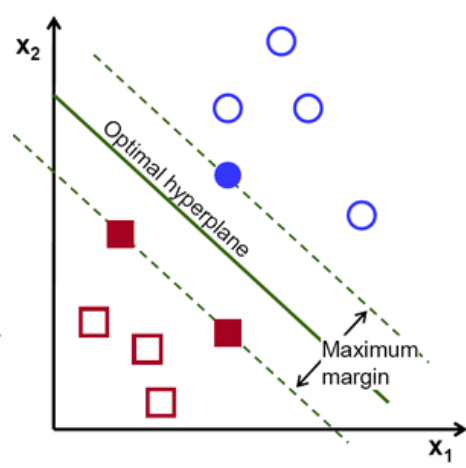
\includegraphics{SVM}
    \caption{The maximum margin in an SVM splits the classes with a boundary such that the distance to the closest sample of each class is maximized. Source: \url{https://cdn-images-1.medium.com/max/2000/1*nUpw5agP-Vefm4Uinteq-A.png}}
    \labfig{SVM}
\end{marginfigure}

The maximum margin is defined as
\begin{align}
    \text{margin} = d_+ + d_-
\end{align}
with $d_+$ the distance to the nearest training sample with class $+1$ and $d_1$ to closest training sample with class $-1$.
Noticeably, this requires the data to be linearly separable, which means that a hyperplane must exist that perfectly separates the data according to its class.
The margin becomes ideal for $d_+ = d_-$.
Since $w$ is orthogonal to the hyperplane, $\vec{w}$ can always be rescaled such that 
\begin{align}
    d_+ = d_- = \frac{1}{\norm{\vec{w}}}
\end{align}

Additionally, $\vec{w}$ can be chosen such that $z = \vec{w}_i^T \vec{x}_i + b_i \geq +1$ for $\tilde{y}_i = +1$ and vice versa for $\tilde{y}_i = -1$.
Thus,
\begin{align}
    \tilde{y}_i z_i \geq 1
\end{align}
will hold, for all inputs $x_i$ with equality for points on the margin, as there is always at least one point of each class on the margin.

Thus,
\begin{align}
    d_- = d_+ = \frac{1}{\norm{\vec{w}}}
\end{align}
and the margin
\begin{align}
    d_- + d_+ = \frac{2}{\norm{\vec{w}}}
    \labeq{maxmargin}
\end{align}
is maximized when $\norm{\vec{w}}$ is minimized.

Subsequently, the classification can be expressed as a relatively simple optimization problem.
\begin{align}
    \argmin_{w, b} \frac{1}{2} \norm{\vec{w}}^2
\end{align}
under the constraints
\begin{align}
    \tilde{y}_i z_i = \tilde{y}_i (\vec{w}_i^T \vec{x} + b) \geq 1 \forall i
    \labeq{constraint}
\end{align}
One way to solve this problem shall be explained in \refch{Optim}.

\subsection{Regularization}
Regularizations, combined with loss functions, penalize possible solutions deemed wrong for any particular reason.
A very common regularization is L2 regularization on the weights.
It is expected that networks with very large weights generalize poorly.
Hence, all weights are summed up and multiplied with a regularization constant $\lambda$ \cite{grosse}.
\begin{align}
	\mathcal{R} = \frac{\lambda}{2} \sum_{i = 1}^D w_i^2
\end{align}

\section{Fully Connected Neural Networks}
\subsection{Multi-Layer Perceptron}
With the perceptron, which is capable of classification any linear separable data, at hand, the question becomes: What are the limitations to this?
\citeauthor{perceptrons} found the limitations in 1969 with their book ``Perceptrons''~\cite{perceptrons}.
They oulined the limitations of perceptrons with the \lstinline|XOR| problem.
The problem becomes obvious when looking at the \lstinline|XOR| problem in a 2D plane (see \reffig{XOR})
\begin{marginfigure}
    \resizebox{\textwidth}{!}{
        %% Creator: Matplotlib, PGF backend
%%
%% To include the figure in your LaTeX document, write
%%   \input{<filename>.pgf}
%%
%% Make sure the required packages are loaded in your preamble
%%   \usepackage{pgf}
%%
%% and, on pdftex
%%   \usepackage[utf8]{inputenc}\DeclareUnicodeCharacter{2212}{-}
%%
%% or, on luatex and xetex
%%   \usepackage{unicode-math}
%%
%% Figures using additional raster images can only be included by \input if
%% they are in the same directory as the main LaTeX file. For loading figures
%% from other directories you can use the `import` package
%%   \usepackage{import}
%%
%% and then include the figures with
%%   \import{<path to file>}{<filename>.pgf}
%%
%% Matplotlib used the following preamble
%%
\begingroup%
\makeatletter%
\begin{pgfpicture}%
\pgfpathrectangle{\pgfpointorigin}{\pgfqpoint{20.000000in}{10.000000in}}%
\pgfusepath{use as bounding box, clip}%
\begin{pgfscope}%
\pgfsetbuttcap%
\pgfsetmiterjoin%
\definecolor{currentfill}{rgb}{1.000000,1.000000,1.000000}%
\pgfsetfillcolor{currentfill}%
\pgfsetlinewidth{0.000000pt}%
\definecolor{currentstroke}{rgb}{1.000000,1.000000,1.000000}%
\pgfsetstrokecolor{currentstroke}%
\pgfsetdash{}{0pt}%
\pgfpathmoveto{\pgfqpoint{0.000000in}{0.000000in}}%
\pgfpathlineto{\pgfqpoint{20.000000in}{0.000000in}}%
\pgfpathlineto{\pgfqpoint{20.000000in}{10.000000in}}%
\pgfpathlineto{\pgfqpoint{0.000000in}{10.000000in}}%
\pgfpathclose%
\pgfusepath{fill}%
\end{pgfscope}%
\begin{pgfscope}%
\pgfsetbuttcap%
\pgfsetmiterjoin%
\definecolor{currentfill}{rgb}{1.000000,1.000000,1.000000}%
\pgfsetfillcolor{currentfill}%
\pgfsetlinewidth{0.000000pt}%
\definecolor{currentstroke}{rgb}{0.000000,0.000000,0.000000}%
\pgfsetstrokecolor{currentstroke}%
\pgfsetstrokeopacity{0.000000}%
\pgfsetdash{}{0pt}%
\pgfpathmoveto{\pgfqpoint{2.500000in}{1.100000in}}%
\pgfpathlineto{\pgfqpoint{9.545455in}{1.100000in}}%
\pgfpathlineto{\pgfqpoint{9.545455in}{8.800000in}}%
\pgfpathlineto{\pgfqpoint{2.500000in}{8.800000in}}%
\pgfpathclose%
\pgfusepath{fill}%
\end{pgfscope}%
\begin{pgfscope}%
\pgfpathrectangle{\pgfqpoint{2.500000in}{1.100000in}}{\pgfqpoint{7.045455in}{7.700000in}}%
\pgfusepath{clip}%
\pgfsetbuttcap%
\pgfsetroundjoin%
\definecolor{currentfill}{rgb}{0.229806,0.298718,0.753683}%
\pgfsetfillcolor{currentfill}%
\pgfsetlinewidth{1.003750pt}%
\definecolor{currentstroke}{rgb}{0.229806,0.298718,0.753683}%
\pgfsetstrokecolor{currentstroke}%
\pgfsetdash{}{0pt}%
\pgfpathmoveto{\pgfqpoint{2.820248in}{1.294718in}}%
\pgfpathcurveto{\pgfqpoint{2.861429in}{1.294718in}}{\pgfqpoint{2.900930in}{1.311079in}}{\pgfqpoint{2.930049in}{1.340199in}}%
\pgfpathcurveto{\pgfqpoint{2.959169in}{1.369318in}}{\pgfqpoint{2.975530in}{1.408819in}}{\pgfqpoint{2.975530in}{1.450000in}}%
\pgfpathcurveto{\pgfqpoint{2.975530in}{1.491181in}}{\pgfqpoint{2.959169in}{1.530682in}}{\pgfqpoint{2.930049in}{1.559801in}}%
\pgfpathcurveto{\pgfqpoint{2.900930in}{1.588921in}}{\pgfqpoint{2.861429in}{1.605282in}}{\pgfqpoint{2.820248in}{1.605282in}}%
\pgfpathcurveto{\pgfqpoint{2.779067in}{1.605282in}}{\pgfqpoint{2.739566in}{1.588921in}}{\pgfqpoint{2.710447in}{1.559801in}}%
\pgfpathcurveto{\pgfqpoint{2.681327in}{1.530682in}}{\pgfqpoint{2.664965in}{1.491181in}}{\pgfqpoint{2.664965in}{1.450000in}}%
\pgfpathcurveto{\pgfqpoint{2.664965in}{1.408819in}}{\pgfqpoint{2.681327in}{1.369318in}}{\pgfqpoint{2.710447in}{1.340199in}}%
\pgfpathcurveto{\pgfqpoint{2.739566in}{1.311079in}}{\pgfqpoint{2.779067in}{1.294718in}}{\pgfqpoint{2.820248in}{1.294718in}}%
\pgfpathclose%
\pgfusepath{stroke,fill}%
\end{pgfscope}%
\begin{pgfscope}%
\pgfpathrectangle{\pgfqpoint{2.500000in}{1.100000in}}{\pgfqpoint{7.045455in}{7.700000in}}%
\pgfusepath{clip}%
\pgfsetbuttcap%
\pgfsetroundjoin%
\definecolor{currentfill}{rgb}{0.705673,0.015556,0.150233}%
\pgfsetfillcolor{currentfill}%
\pgfsetlinewidth{1.003750pt}%
\definecolor{currentstroke}{rgb}{0.705673,0.015556,0.150233}%
\pgfsetstrokecolor{currentstroke}%
\pgfsetdash{}{0pt}%
\pgfpathmoveto{\pgfqpoint{9.225207in}{8.294718in}}%
\pgfpathcurveto{\pgfqpoint{9.266388in}{8.294718in}}{\pgfqpoint{9.305888in}{8.311079in}}{\pgfqpoint{9.335008in}{8.340199in}}%
\pgfpathcurveto{\pgfqpoint{9.364128in}{8.369318in}}{\pgfqpoint{9.380489in}{8.408819in}}{\pgfqpoint{9.380489in}{8.450000in}}%
\pgfpathcurveto{\pgfqpoint{9.380489in}{8.491181in}}{\pgfqpoint{9.364128in}{8.530682in}}{\pgfqpoint{9.335008in}{8.559801in}}%
\pgfpathcurveto{\pgfqpoint{9.305888in}{8.588921in}}{\pgfqpoint{9.266388in}{8.605282in}}{\pgfqpoint{9.225207in}{8.605282in}}%
\pgfpathcurveto{\pgfqpoint{9.184025in}{8.605282in}}{\pgfqpoint{9.144525in}{8.588921in}}{\pgfqpoint{9.115405in}{8.559801in}}%
\pgfpathcurveto{\pgfqpoint{9.086286in}{8.530682in}}{\pgfqpoint{9.069924in}{8.491181in}}{\pgfqpoint{9.069924in}{8.450000in}}%
\pgfpathcurveto{\pgfqpoint{9.069924in}{8.408819in}}{\pgfqpoint{9.086286in}{8.369318in}}{\pgfqpoint{9.115405in}{8.340199in}}%
\pgfpathcurveto{\pgfqpoint{9.144525in}{8.311079in}}{\pgfqpoint{9.184025in}{8.294718in}}{\pgfqpoint{9.225207in}{8.294718in}}%
\pgfpathclose%
\pgfusepath{stroke,fill}%
\end{pgfscope}%
\begin{pgfscope}%
\pgfpathrectangle{\pgfqpoint{2.500000in}{1.100000in}}{\pgfqpoint{7.045455in}{7.700000in}}%
\pgfusepath{clip}%
\pgfsetbuttcap%
\pgfsetroundjoin%
\definecolor{currentfill}{rgb}{0.705673,0.015556,0.150233}%
\pgfsetfillcolor{currentfill}%
\pgfsetlinewidth{1.003750pt}%
\definecolor{currentstroke}{rgb}{0.705673,0.015556,0.150233}%
\pgfsetstrokecolor{currentstroke}%
\pgfsetdash{}{0pt}%
\pgfpathmoveto{\pgfqpoint{9.225207in}{1.294718in}}%
\pgfpathcurveto{\pgfqpoint{9.266388in}{1.294718in}}{\pgfqpoint{9.305888in}{1.311079in}}{\pgfqpoint{9.335008in}{1.340199in}}%
\pgfpathcurveto{\pgfqpoint{9.364128in}{1.369318in}}{\pgfqpoint{9.380489in}{1.408819in}}{\pgfqpoint{9.380489in}{1.450000in}}%
\pgfpathcurveto{\pgfqpoint{9.380489in}{1.491181in}}{\pgfqpoint{9.364128in}{1.530682in}}{\pgfqpoint{9.335008in}{1.559801in}}%
\pgfpathcurveto{\pgfqpoint{9.305888in}{1.588921in}}{\pgfqpoint{9.266388in}{1.605282in}}{\pgfqpoint{9.225207in}{1.605282in}}%
\pgfpathcurveto{\pgfqpoint{9.184025in}{1.605282in}}{\pgfqpoint{9.144525in}{1.588921in}}{\pgfqpoint{9.115405in}{1.559801in}}%
\pgfpathcurveto{\pgfqpoint{9.086286in}{1.530682in}}{\pgfqpoint{9.069924in}{1.491181in}}{\pgfqpoint{9.069924in}{1.450000in}}%
\pgfpathcurveto{\pgfqpoint{9.069924in}{1.408819in}}{\pgfqpoint{9.086286in}{1.369318in}}{\pgfqpoint{9.115405in}{1.340199in}}%
\pgfpathcurveto{\pgfqpoint{9.144525in}{1.311079in}}{\pgfqpoint{9.184025in}{1.294718in}}{\pgfqpoint{9.225207in}{1.294718in}}%
\pgfpathclose%
\pgfusepath{stroke,fill}%
\end{pgfscope}%
\begin{pgfscope}%
\pgfpathrectangle{\pgfqpoint{2.500000in}{1.100000in}}{\pgfqpoint{7.045455in}{7.700000in}}%
\pgfusepath{clip}%
\pgfsetbuttcap%
\pgfsetroundjoin%
\definecolor{currentfill}{rgb}{0.705673,0.015556,0.150233}%
\pgfsetfillcolor{currentfill}%
\pgfsetlinewidth{1.003750pt}%
\definecolor{currentstroke}{rgb}{0.705673,0.015556,0.150233}%
\pgfsetstrokecolor{currentstroke}%
\pgfsetdash{}{0pt}%
\pgfpathmoveto{\pgfqpoint{2.820248in}{8.294718in}}%
\pgfpathcurveto{\pgfqpoint{2.861429in}{8.294718in}}{\pgfqpoint{2.900930in}{8.311079in}}{\pgfqpoint{2.930049in}{8.340199in}}%
\pgfpathcurveto{\pgfqpoint{2.959169in}{8.369318in}}{\pgfqpoint{2.975530in}{8.408819in}}{\pgfqpoint{2.975530in}{8.450000in}}%
\pgfpathcurveto{\pgfqpoint{2.975530in}{8.491181in}}{\pgfqpoint{2.959169in}{8.530682in}}{\pgfqpoint{2.930049in}{8.559801in}}%
\pgfpathcurveto{\pgfqpoint{2.900930in}{8.588921in}}{\pgfqpoint{2.861429in}{8.605282in}}{\pgfqpoint{2.820248in}{8.605282in}}%
\pgfpathcurveto{\pgfqpoint{2.779067in}{8.605282in}}{\pgfqpoint{2.739566in}{8.588921in}}{\pgfqpoint{2.710447in}{8.559801in}}%
\pgfpathcurveto{\pgfqpoint{2.681327in}{8.530682in}}{\pgfqpoint{2.664965in}{8.491181in}}{\pgfqpoint{2.664965in}{8.450000in}}%
\pgfpathcurveto{\pgfqpoint{2.664965in}{8.408819in}}{\pgfqpoint{2.681327in}{8.369318in}}{\pgfqpoint{2.710447in}{8.340199in}}%
\pgfpathcurveto{\pgfqpoint{2.739566in}{8.311079in}}{\pgfqpoint{2.779067in}{8.294718in}}{\pgfqpoint{2.820248in}{8.294718in}}%
\pgfpathclose%
\pgfusepath{stroke,fill}%
\end{pgfscope}%
\begin{pgfscope}%
\pgfsetbuttcap%
\pgfsetroundjoin%
\definecolor{currentfill}{rgb}{0.000000,0.000000,0.000000}%
\pgfsetfillcolor{currentfill}%
\pgfsetlinewidth{0.803000pt}%
\definecolor{currentstroke}{rgb}{0.000000,0.000000,0.000000}%
\pgfsetstrokecolor{currentstroke}%
\pgfsetdash{}{0pt}%
\pgfsys@defobject{currentmarker}{\pgfqpoint{0.000000in}{-0.048611in}}{\pgfqpoint{0.000000in}{0.000000in}}{%
\pgfpathmoveto{\pgfqpoint{0.000000in}{0.000000in}}%
\pgfpathlineto{\pgfqpoint{0.000000in}{-0.048611in}}%
\pgfusepath{stroke,fill}%
}%
\begin{pgfscope}%
\pgfsys@transformshift{9.225207in}{1.100000in}%
\pgfsys@useobject{currentmarker}{}%
\end{pgfscope}%
\end{pgfscope}%
\begin{pgfscope}%
\definecolor{textcolor}{rgb}{0.000000,0.000000,0.000000}%
\pgfsetstrokecolor{textcolor}%
\pgfsetfillcolor{textcolor}%
\pgftext[x=9.225207in,y=1.002778in,,top]{\color{textcolor}\rmfamily\fontsize{10.000000}{12.000000}\selectfont True}%
\end{pgfscope}%
\begin{pgfscope}%
\pgfsetbuttcap%
\pgfsetroundjoin%
\definecolor{currentfill}{rgb}{0.000000,0.000000,0.000000}%
\pgfsetfillcolor{currentfill}%
\pgfsetlinewidth{0.803000pt}%
\definecolor{currentstroke}{rgb}{0.000000,0.000000,0.000000}%
\pgfsetstrokecolor{currentstroke}%
\pgfsetdash{}{0pt}%
\pgfsys@defobject{currentmarker}{\pgfqpoint{0.000000in}{-0.048611in}}{\pgfqpoint{0.000000in}{0.000000in}}{%
\pgfpathmoveto{\pgfqpoint{0.000000in}{0.000000in}}%
\pgfpathlineto{\pgfqpoint{0.000000in}{-0.048611in}}%
\pgfusepath{stroke,fill}%
}%
\begin{pgfscope}%
\pgfsys@transformshift{2.820248in}{1.100000in}%
\pgfsys@useobject{currentmarker}{}%
\end{pgfscope}%
\end{pgfscope}%
\begin{pgfscope}%
\definecolor{textcolor}{rgb}{0.000000,0.000000,0.000000}%
\pgfsetstrokecolor{textcolor}%
\pgfsetfillcolor{textcolor}%
\pgftext[x=2.820248in,y=1.002778in,,top]{\color{textcolor}\rmfamily\fontsize{10.000000}{12.000000}\selectfont False}%
\end{pgfscope}%
\begin{pgfscope}%
\definecolor{textcolor}{rgb}{0.000000,0.000000,0.000000}%
\pgfsetstrokecolor{textcolor}%
\pgfsetfillcolor{textcolor}%
\pgftext[x=6.022727in,y=0.823766in,,top]{\color{textcolor}\rmfamily\fontsize{10.000000}{12.000000}\selectfont \(\displaystyle x_1\)}%
\end{pgfscope}%
\begin{pgfscope}%
\pgfsetbuttcap%
\pgfsetroundjoin%
\definecolor{currentfill}{rgb}{0.000000,0.000000,0.000000}%
\pgfsetfillcolor{currentfill}%
\pgfsetlinewidth{0.803000pt}%
\definecolor{currentstroke}{rgb}{0.000000,0.000000,0.000000}%
\pgfsetstrokecolor{currentstroke}%
\pgfsetdash{}{0pt}%
\pgfsys@defobject{currentmarker}{\pgfqpoint{-0.048611in}{0.000000in}}{\pgfqpoint{0.000000in}{0.000000in}}{%
\pgfpathmoveto{\pgfqpoint{0.000000in}{0.000000in}}%
\pgfpathlineto{\pgfqpoint{-0.048611in}{0.000000in}}%
\pgfusepath{stroke,fill}%
}%
\begin{pgfscope}%
\pgfsys@transformshift{2.500000in}{8.450000in}%
\pgfsys@useobject{currentmarker}{}%
\end{pgfscope}%
\end{pgfscope}%
\begin{pgfscope}%
\definecolor{textcolor}{rgb}{0.000000,0.000000,0.000000}%
\pgfsetstrokecolor{textcolor}%
\pgfsetfillcolor{textcolor}%
\pgftext[x=2.120756in, y=8.401775in, left, base]{\color{textcolor}\rmfamily\fontsize{10.000000}{12.000000}\selectfont True}%
\end{pgfscope}%
\begin{pgfscope}%
\pgfsetbuttcap%
\pgfsetroundjoin%
\definecolor{currentfill}{rgb}{0.000000,0.000000,0.000000}%
\pgfsetfillcolor{currentfill}%
\pgfsetlinewidth{0.803000pt}%
\definecolor{currentstroke}{rgb}{0.000000,0.000000,0.000000}%
\pgfsetstrokecolor{currentstroke}%
\pgfsetdash{}{0pt}%
\pgfsys@defobject{currentmarker}{\pgfqpoint{-0.048611in}{0.000000in}}{\pgfqpoint{0.000000in}{0.000000in}}{%
\pgfpathmoveto{\pgfqpoint{0.000000in}{0.000000in}}%
\pgfpathlineto{\pgfqpoint{-0.048611in}{0.000000in}}%
\pgfusepath{stroke,fill}%
}%
\begin{pgfscope}%
\pgfsys@transformshift{2.500000in}{1.450000in}%
\pgfsys@useobject{currentmarker}{}%
\end{pgfscope}%
\end{pgfscope}%
\begin{pgfscope}%
\definecolor{textcolor}{rgb}{0.000000,0.000000,0.000000}%
\pgfsetstrokecolor{textcolor}%
\pgfsetfillcolor{textcolor}%
\pgftext[x=2.099151in, y=1.401775in, left, base]{\color{textcolor}\rmfamily\fontsize{10.000000}{12.000000}\selectfont False}%
\end{pgfscope}%
\begin{pgfscope}%
\definecolor{textcolor}{rgb}{0.000000,0.000000,0.000000}%
\pgfsetstrokecolor{textcolor}%
\pgfsetfillcolor{textcolor}%
\pgftext[x=2.043595in,y=4.950000in,,bottom,rotate=90.000000]{\color{textcolor}\rmfamily\fontsize{10.000000}{12.000000}\selectfont \(\displaystyle x_2\)}%
\end{pgfscope}%
\begin{pgfscope}%
\pgfsetrectcap%
\pgfsetmiterjoin%
\pgfsetlinewidth{0.803000pt}%
\definecolor{currentstroke}{rgb}{0.000000,0.000000,0.000000}%
\pgfsetstrokecolor{currentstroke}%
\pgfsetdash{}{0pt}%
\pgfpathmoveto{\pgfqpoint{2.500000in}{1.100000in}}%
\pgfpathlineto{\pgfqpoint{2.500000in}{8.800000in}}%
\pgfusepath{stroke}%
\end{pgfscope}%
\begin{pgfscope}%
\pgfsetrectcap%
\pgfsetmiterjoin%
\pgfsetlinewidth{0.803000pt}%
\definecolor{currentstroke}{rgb}{0.000000,0.000000,0.000000}%
\pgfsetstrokecolor{currentstroke}%
\pgfsetdash{}{0pt}%
\pgfpathmoveto{\pgfqpoint{9.545455in}{1.100000in}}%
\pgfpathlineto{\pgfqpoint{9.545455in}{8.800000in}}%
\pgfusepath{stroke}%
\end{pgfscope}%
\begin{pgfscope}%
\pgfsetrectcap%
\pgfsetmiterjoin%
\pgfsetlinewidth{0.803000pt}%
\definecolor{currentstroke}{rgb}{0.000000,0.000000,0.000000}%
\pgfsetstrokecolor{currentstroke}%
\pgfsetdash{}{0pt}%
\pgfpathmoveto{\pgfqpoint{2.500000in}{1.100000in}}%
\pgfpathlineto{\pgfqpoint{9.545455in}{1.100000in}}%
\pgfusepath{stroke}%
\end{pgfscope}%
\begin{pgfscope}%
\pgfsetrectcap%
\pgfsetmiterjoin%
\pgfsetlinewidth{0.803000pt}%
\definecolor{currentstroke}{rgb}{0.000000,0.000000,0.000000}%
\pgfsetstrokecolor{currentstroke}%
\pgfsetdash{}{0pt}%
\pgfpathmoveto{\pgfqpoint{2.500000in}{8.800000in}}%
\pgfpathlineto{\pgfqpoint{9.545455in}{8.800000in}}%
\pgfusepath{stroke}%
\end{pgfscope}%
\begin{pgfscope}%
\definecolor{textcolor}{rgb}{0.000000,0.000000,0.000000}%
\pgfsetstrokecolor{textcolor}%
\pgfsetfillcolor{textcolor}%
\pgftext[x=6.022727in,y=8.883333in,,base]{\color{textcolor}\rmfamily\fontsize{12.000000}{14.400000}\selectfont OR}%
\end{pgfscope}%
\begin{pgfscope}%
\pgfsetbuttcap%
\pgfsetmiterjoin%
\definecolor{currentfill}{rgb}{1.000000,1.000000,1.000000}%
\pgfsetfillcolor{currentfill}%
\pgfsetlinewidth{0.000000pt}%
\definecolor{currentstroke}{rgb}{0.000000,0.000000,0.000000}%
\pgfsetstrokecolor{currentstroke}%
\pgfsetstrokeopacity{0.000000}%
\pgfsetdash{}{0pt}%
\pgfpathmoveto{\pgfqpoint{10.954545in}{1.100000in}}%
\pgfpathlineto{\pgfqpoint{18.000000in}{1.100000in}}%
\pgfpathlineto{\pgfqpoint{18.000000in}{8.800000in}}%
\pgfpathlineto{\pgfqpoint{10.954545in}{8.800000in}}%
\pgfpathclose%
\pgfusepath{fill}%
\end{pgfscope}%
\begin{pgfscope}%
\pgfpathrectangle{\pgfqpoint{10.954545in}{1.100000in}}{\pgfqpoint{7.045455in}{7.700000in}}%
\pgfusepath{clip}%
\pgfsetbuttcap%
\pgfsetroundjoin%
\definecolor{currentfill}{rgb}{0.229806,0.298718,0.753683}%
\pgfsetfillcolor{currentfill}%
\pgfsetlinewidth{1.003750pt}%
\definecolor{currentstroke}{rgb}{0.229806,0.298718,0.753683}%
\pgfsetstrokecolor{currentstroke}%
\pgfsetdash{}{0pt}%
\pgfpathmoveto{\pgfqpoint{11.274793in}{1.294718in}}%
\pgfpathcurveto{\pgfqpoint{11.315975in}{1.294718in}}{\pgfqpoint{11.355475in}{1.311079in}}{\pgfqpoint{11.384595in}{1.340199in}}%
\pgfpathcurveto{\pgfqpoint{11.413714in}{1.369318in}}{\pgfqpoint{11.430076in}{1.408819in}}{\pgfqpoint{11.430076in}{1.450000in}}%
\pgfpathcurveto{\pgfqpoint{11.430076in}{1.491181in}}{\pgfqpoint{11.413714in}{1.530682in}}{\pgfqpoint{11.384595in}{1.559801in}}%
\pgfpathcurveto{\pgfqpoint{11.355475in}{1.588921in}}{\pgfqpoint{11.315975in}{1.605282in}}{\pgfqpoint{11.274793in}{1.605282in}}%
\pgfpathcurveto{\pgfqpoint{11.233612in}{1.605282in}}{\pgfqpoint{11.194112in}{1.588921in}}{\pgfqpoint{11.164992in}{1.559801in}}%
\pgfpathcurveto{\pgfqpoint{11.135872in}{1.530682in}}{\pgfqpoint{11.119511in}{1.491181in}}{\pgfqpoint{11.119511in}{1.450000in}}%
\pgfpathcurveto{\pgfqpoint{11.119511in}{1.408819in}}{\pgfqpoint{11.135872in}{1.369318in}}{\pgfqpoint{11.164992in}{1.340199in}}%
\pgfpathcurveto{\pgfqpoint{11.194112in}{1.311079in}}{\pgfqpoint{11.233612in}{1.294718in}}{\pgfqpoint{11.274793in}{1.294718in}}%
\pgfpathclose%
\pgfusepath{stroke,fill}%
\end{pgfscope}%
\begin{pgfscope}%
\pgfpathrectangle{\pgfqpoint{10.954545in}{1.100000in}}{\pgfqpoint{7.045455in}{7.700000in}}%
\pgfusepath{clip}%
\pgfsetbuttcap%
\pgfsetroundjoin%
\definecolor{currentfill}{rgb}{0.229806,0.298718,0.753683}%
\pgfsetfillcolor{currentfill}%
\pgfsetlinewidth{1.003750pt}%
\definecolor{currentstroke}{rgb}{0.229806,0.298718,0.753683}%
\pgfsetstrokecolor{currentstroke}%
\pgfsetdash{}{0pt}%
\pgfpathmoveto{\pgfqpoint{17.679752in}{8.294718in}}%
\pgfpathcurveto{\pgfqpoint{17.720933in}{8.294718in}}{\pgfqpoint{17.760434in}{8.311079in}}{\pgfqpoint{17.789553in}{8.340199in}}%
\pgfpathcurveto{\pgfqpoint{17.818673in}{8.369318in}}{\pgfqpoint{17.835035in}{8.408819in}}{\pgfqpoint{17.835035in}{8.450000in}}%
\pgfpathcurveto{\pgfqpoint{17.835035in}{8.491181in}}{\pgfqpoint{17.818673in}{8.530682in}}{\pgfqpoint{17.789553in}{8.559801in}}%
\pgfpathcurveto{\pgfqpoint{17.760434in}{8.588921in}}{\pgfqpoint{17.720933in}{8.605282in}}{\pgfqpoint{17.679752in}{8.605282in}}%
\pgfpathcurveto{\pgfqpoint{17.638571in}{8.605282in}}{\pgfqpoint{17.599070in}{8.588921in}}{\pgfqpoint{17.569951in}{8.559801in}}%
\pgfpathcurveto{\pgfqpoint{17.540831in}{8.530682in}}{\pgfqpoint{17.524470in}{8.491181in}}{\pgfqpoint{17.524470in}{8.450000in}}%
\pgfpathcurveto{\pgfqpoint{17.524470in}{8.408819in}}{\pgfqpoint{17.540831in}{8.369318in}}{\pgfqpoint{17.569951in}{8.340199in}}%
\pgfpathcurveto{\pgfqpoint{17.599070in}{8.311079in}}{\pgfqpoint{17.638571in}{8.294718in}}{\pgfqpoint{17.679752in}{8.294718in}}%
\pgfpathclose%
\pgfusepath{stroke,fill}%
\end{pgfscope}%
\begin{pgfscope}%
\pgfpathrectangle{\pgfqpoint{10.954545in}{1.100000in}}{\pgfqpoint{7.045455in}{7.700000in}}%
\pgfusepath{clip}%
\pgfsetbuttcap%
\pgfsetroundjoin%
\definecolor{currentfill}{rgb}{0.705673,0.015556,0.150233}%
\pgfsetfillcolor{currentfill}%
\pgfsetlinewidth{1.003750pt}%
\definecolor{currentstroke}{rgb}{0.705673,0.015556,0.150233}%
\pgfsetstrokecolor{currentstroke}%
\pgfsetdash{}{0pt}%
\pgfpathmoveto{\pgfqpoint{17.679752in}{1.294718in}}%
\pgfpathcurveto{\pgfqpoint{17.720933in}{1.294718in}}{\pgfqpoint{17.760434in}{1.311079in}}{\pgfqpoint{17.789553in}{1.340199in}}%
\pgfpathcurveto{\pgfqpoint{17.818673in}{1.369318in}}{\pgfqpoint{17.835035in}{1.408819in}}{\pgfqpoint{17.835035in}{1.450000in}}%
\pgfpathcurveto{\pgfqpoint{17.835035in}{1.491181in}}{\pgfqpoint{17.818673in}{1.530682in}}{\pgfqpoint{17.789553in}{1.559801in}}%
\pgfpathcurveto{\pgfqpoint{17.760434in}{1.588921in}}{\pgfqpoint{17.720933in}{1.605282in}}{\pgfqpoint{17.679752in}{1.605282in}}%
\pgfpathcurveto{\pgfqpoint{17.638571in}{1.605282in}}{\pgfqpoint{17.599070in}{1.588921in}}{\pgfqpoint{17.569951in}{1.559801in}}%
\pgfpathcurveto{\pgfqpoint{17.540831in}{1.530682in}}{\pgfqpoint{17.524470in}{1.491181in}}{\pgfqpoint{17.524470in}{1.450000in}}%
\pgfpathcurveto{\pgfqpoint{17.524470in}{1.408819in}}{\pgfqpoint{17.540831in}{1.369318in}}{\pgfqpoint{17.569951in}{1.340199in}}%
\pgfpathcurveto{\pgfqpoint{17.599070in}{1.311079in}}{\pgfqpoint{17.638571in}{1.294718in}}{\pgfqpoint{17.679752in}{1.294718in}}%
\pgfpathclose%
\pgfusepath{stroke,fill}%
\end{pgfscope}%
\begin{pgfscope}%
\pgfpathrectangle{\pgfqpoint{10.954545in}{1.100000in}}{\pgfqpoint{7.045455in}{7.700000in}}%
\pgfusepath{clip}%
\pgfsetbuttcap%
\pgfsetroundjoin%
\definecolor{currentfill}{rgb}{0.705673,0.015556,0.150233}%
\pgfsetfillcolor{currentfill}%
\pgfsetlinewidth{1.003750pt}%
\definecolor{currentstroke}{rgb}{0.705673,0.015556,0.150233}%
\pgfsetstrokecolor{currentstroke}%
\pgfsetdash{}{0pt}%
\pgfpathmoveto{\pgfqpoint{11.274793in}{8.294718in}}%
\pgfpathcurveto{\pgfqpoint{11.315975in}{8.294718in}}{\pgfqpoint{11.355475in}{8.311079in}}{\pgfqpoint{11.384595in}{8.340199in}}%
\pgfpathcurveto{\pgfqpoint{11.413714in}{8.369318in}}{\pgfqpoint{11.430076in}{8.408819in}}{\pgfqpoint{11.430076in}{8.450000in}}%
\pgfpathcurveto{\pgfqpoint{11.430076in}{8.491181in}}{\pgfqpoint{11.413714in}{8.530682in}}{\pgfqpoint{11.384595in}{8.559801in}}%
\pgfpathcurveto{\pgfqpoint{11.355475in}{8.588921in}}{\pgfqpoint{11.315975in}{8.605282in}}{\pgfqpoint{11.274793in}{8.605282in}}%
\pgfpathcurveto{\pgfqpoint{11.233612in}{8.605282in}}{\pgfqpoint{11.194112in}{8.588921in}}{\pgfqpoint{11.164992in}{8.559801in}}%
\pgfpathcurveto{\pgfqpoint{11.135872in}{8.530682in}}{\pgfqpoint{11.119511in}{8.491181in}}{\pgfqpoint{11.119511in}{8.450000in}}%
\pgfpathcurveto{\pgfqpoint{11.119511in}{8.408819in}}{\pgfqpoint{11.135872in}{8.369318in}}{\pgfqpoint{11.164992in}{8.340199in}}%
\pgfpathcurveto{\pgfqpoint{11.194112in}{8.311079in}}{\pgfqpoint{11.233612in}{8.294718in}}{\pgfqpoint{11.274793in}{8.294718in}}%
\pgfpathclose%
\pgfusepath{stroke,fill}%
\end{pgfscope}%
\begin{pgfscope}%
\pgfsetbuttcap%
\pgfsetroundjoin%
\definecolor{currentfill}{rgb}{0.000000,0.000000,0.000000}%
\pgfsetfillcolor{currentfill}%
\pgfsetlinewidth{0.803000pt}%
\definecolor{currentstroke}{rgb}{0.000000,0.000000,0.000000}%
\pgfsetstrokecolor{currentstroke}%
\pgfsetdash{}{0pt}%
\pgfsys@defobject{currentmarker}{\pgfqpoint{0.000000in}{-0.048611in}}{\pgfqpoint{0.000000in}{0.000000in}}{%
\pgfpathmoveto{\pgfqpoint{0.000000in}{0.000000in}}%
\pgfpathlineto{\pgfqpoint{0.000000in}{-0.048611in}}%
\pgfusepath{stroke,fill}%
}%
\begin{pgfscope}%
\pgfsys@transformshift{17.679752in}{1.100000in}%
\pgfsys@useobject{currentmarker}{}%
\end{pgfscope}%
\end{pgfscope}%
\begin{pgfscope}%
\definecolor{textcolor}{rgb}{0.000000,0.000000,0.000000}%
\pgfsetstrokecolor{textcolor}%
\pgfsetfillcolor{textcolor}%
\pgftext[x=17.679752in,y=1.002778in,,top]{\color{textcolor}\rmfamily\fontsize{10.000000}{12.000000}\selectfont True}%
\end{pgfscope}%
\begin{pgfscope}%
\pgfsetbuttcap%
\pgfsetroundjoin%
\definecolor{currentfill}{rgb}{0.000000,0.000000,0.000000}%
\pgfsetfillcolor{currentfill}%
\pgfsetlinewidth{0.803000pt}%
\definecolor{currentstroke}{rgb}{0.000000,0.000000,0.000000}%
\pgfsetstrokecolor{currentstroke}%
\pgfsetdash{}{0pt}%
\pgfsys@defobject{currentmarker}{\pgfqpoint{0.000000in}{-0.048611in}}{\pgfqpoint{0.000000in}{0.000000in}}{%
\pgfpathmoveto{\pgfqpoint{0.000000in}{0.000000in}}%
\pgfpathlineto{\pgfqpoint{0.000000in}{-0.048611in}}%
\pgfusepath{stroke,fill}%
}%
\begin{pgfscope}%
\pgfsys@transformshift{11.274793in}{1.100000in}%
\pgfsys@useobject{currentmarker}{}%
\end{pgfscope}%
\end{pgfscope}%
\begin{pgfscope}%
\definecolor{textcolor}{rgb}{0.000000,0.000000,0.000000}%
\pgfsetstrokecolor{textcolor}%
\pgfsetfillcolor{textcolor}%
\pgftext[x=11.274793in,y=1.002778in,,top]{\color{textcolor}\rmfamily\fontsize{10.000000}{12.000000}\selectfont False}%
\end{pgfscope}%
\begin{pgfscope}%
\definecolor{textcolor}{rgb}{0.000000,0.000000,0.000000}%
\pgfsetstrokecolor{textcolor}%
\pgfsetfillcolor{textcolor}%
\pgftext[x=14.477273in,y=0.823766in,,top]{\color{textcolor}\rmfamily\fontsize{10.000000}{12.000000}\selectfont \(\displaystyle x_1\)}%
\end{pgfscope}%
\begin{pgfscope}%
\pgfsetbuttcap%
\pgfsetroundjoin%
\definecolor{currentfill}{rgb}{0.000000,0.000000,0.000000}%
\pgfsetfillcolor{currentfill}%
\pgfsetlinewidth{0.803000pt}%
\definecolor{currentstroke}{rgb}{0.000000,0.000000,0.000000}%
\pgfsetstrokecolor{currentstroke}%
\pgfsetdash{}{0pt}%
\pgfsys@defobject{currentmarker}{\pgfqpoint{-0.048611in}{0.000000in}}{\pgfqpoint{0.000000in}{0.000000in}}{%
\pgfpathmoveto{\pgfqpoint{0.000000in}{0.000000in}}%
\pgfpathlineto{\pgfqpoint{-0.048611in}{0.000000in}}%
\pgfusepath{stroke,fill}%
}%
\begin{pgfscope}%
\pgfsys@transformshift{10.954545in}{8.450000in}%
\pgfsys@useobject{currentmarker}{}%
\end{pgfscope}%
\end{pgfscope}%
\begin{pgfscope}%
\definecolor{textcolor}{rgb}{0.000000,0.000000,0.000000}%
\pgfsetstrokecolor{textcolor}%
\pgfsetfillcolor{textcolor}%
\pgftext[x=10.575301in, y=8.401775in, left, base]{\color{textcolor}\rmfamily\fontsize{10.000000}{12.000000}\selectfont True}%
\end{pgfscope}%
\begin{pgfscope}%
\pgfsetbuttcap%
\pgfsetroundjoin%
\definecolor{currentfill}{rgb}{0.000000,0.000000,0.000000}%
\pgfsetfillcolor{currentfill}%
\pgfsetlinewidth{0.803000pt}%
\definecolor{currentstroke}{rgb}{0.000000,0.000000,0.000000}%
\pgfsetstrokecolor{currentstroke}%
\pgfsetdash{}{0pt}%
\pgfsys@defobject{currentmarker}{\pgfqpoint{-0.048611in}{0.000000in}}{\pgfqpoint{0.000000in}{0.000000in}}{%
\pgfpathmoveto{\pgfqpoint{0.000000in}{0.000000in}}%
\pgfpathlineto{\pgfqpoint{-0.048611in}{0.000000in}}%
\pgfusepath{stroke,fill}%
}%
\begin{pgfscope}%
\pgfsys@transformshift{10.954545in}{1.450000in}%
\pgfsys@useobject{currentmarker}{}%
\end{pgfscope}%
\end{pgfscope}%
\begin{pgfscope}%
\definecolor{textcolor}{rgb}{0.000000,0.000000,0.000000}%
\pgfsetstrokecolor{textcolor}%
\pgfsetfillcolor{textcolor}%
\pgftext[x=10.553696in, y=1.401775in, left, base]{\color{textcolor}\rmfamily\fontsize{10.000000}{12.000000}\selectfont False}%
\end{pgfscope}%
\begin{pgfscope}%
\definecolor{textcolor}{rgb}{0.000000,0.000000,0.000000}%
\pgfsetstrokecolor{textcolor}%
\pgfsetfillcolor{textcolor}%
\pgftext[x=10.498141in,y=4.950000in,,bottom,rotate=90.000000]{\color{textcolor}\rmfamily\fontsize{10.000000}{12.000000}\selectfont \(\displaystyle x_2\)}%
\end{pgfscope}%
\begin{pgfscope}%
\pgfsetrectcap%
\pgfsetmiterjoin%
\pgfsetlinewidth{0.803000pt}%
\definecolor{currentstroke}{rgb}{0.000000,0.000000,0.000000}%
\pgfsetstrokecolor{currentstroke}%
\pgfsetdash{}{0pt}%
\pgfpathmoveto{\pgfqpoint{10.954545in}{1.100000in}}%
\pgfpathlineto{\pgfqpoint{10.954545in}{8.800000in}}%
\pgfusepath{stroke}%
\end{pgfscope}%
\begin{pgfscope}%
\pgfsetrectcap%
\pgfsetmiterjoin%
\pgfsetlinewidth{0.803000pt}%
\definecolor{currentstroke}{rgb}{0.000000,0.000000,0.000000}%
\pgfsetstrokecolor{currentstroke}%
\pgfsetdash{}{0pt}%
\pgfpathmoveto{\pgfqpoint{18.000000in}{1.100000in}}%
\pgfpathlineto{\pgfqpoint{18.000000in}{8.800000in}}%
\pgfusepath{stroke}%
\end{pgfscope}%
\begin{pgfscope}%
\pgfsetrectcap%
\pgfsetmiterjoin%
\pgfsetlinewidth{0.803000pt}%
\definecolor{currentstroke}{rgb}{0.000000,0.000000,0.000000}%
\pgfsetstrokecolor{currentstroke}%
\pgfsetdash{}{0pt}%
\pgfpathmoveto{\pgfqpoint{10.954545in}{1.100000in}}%
\pgfpathlineto{\pgfqpoint{18.000000in}{1.100000in}}%
\pgfusepath{stroke}%
\end{pgfscope}%
\begin{pgfscope}%
\pgfsetrectcap%
\pgfsetmiterjoin%
\pgfsetlinewidth{0.803000pt}%
\definecolor{currentstroke}{rgb}{0.000000,0.000000,0.000000}%
\pgfsetstrokecolor{currentstroke}%
\pgfsetdash{}{0pt}%
\pgfpathmoveto{\pgfqpoint{10.954545in}{8.800000in}}%
\pgfpathlineto{\pgfqpoint{18.000000in}{8.800000in}}%
\pgfusepath{stroke}%
\end{pgfscope}%
\begin{pgfscope}%
\definecolor{textcolor}{rgb}{0.000000,0.000000,0.000000}%
\pgfsetstrokecolor{textcolor}%
\pgfsetfillcolor{textcolor}%
\pgftext[x=14.477273in,y=8.883333in,,base]{\color{textcolor}\rmfamily\fontsize{12.000000}{14.400000}\selectfont XOR}%
\end{pgfscope}%
\end{pgfpicture}%
\makeatother%
\endgroup%

    }
    \caption{\lstinline|OR| and \lstinline|XOR| operations visualized. The \lstinline|XOR| problem cannot be solved by drawing a single line.}
    \labfig{XOR}
\end{marginfigure}

As it has been explained in the previous section, the perceptron is equal to a binary linear classifier.
As such, the perceptron can only classify linear separable data perfectly.
Since the \lstinline|XOR| problem can obviously not be solved with a straight line separating the two classes, the perceptron is also not able to compute such an operation. 

This realization led to the first decline in interest in artificial neural networks.

Since then, there have been ways of solving this problem for SVMs by projecting the data into a higher dimensional space with various kernel functions \cite{ommer}.
Another approach keeps the logic but goes from the shallow network approach to a deep neural network (DNN).
\textbf{Deep Neural Networks (DNN)} are ANNs which consist of more than one hidden layer.
A single perceptron may not be capable of computing \lstinline|XOR| but it is capable of calculating \lstinline|AND|, \lstinline|OR| and their negated forms.
By using one perceptron with two units to compute \lstinline|AND| and \lstinline|OR|, a second layer perceptron can in fact compute \lstinline|XOR|
\begin{align}
    XOR(x, y) = AND(OR(x, y), NOT(AND(x, y)))
\end{align}

Thus, DNNs solve the \lstinline|XOR| problem.

\marginnote{The ability to stack \textit{and train} multiple layers in ANNs stems from the discovery of backpropagation which shall be explained in \refsec{backprop}.}

Perceptrons, until then, could approximate only linear functions.
Multiple layers of perceptrons now promise to approximate any higher degree function just as well.
Thus, \textbf{Multi-Layer Perceptrons (MLP)} sparked new interest in the field of artificial neural networks.

This interest also originated in the similarly layered structure that has been found in the brain.
\begin{marginfigure}
    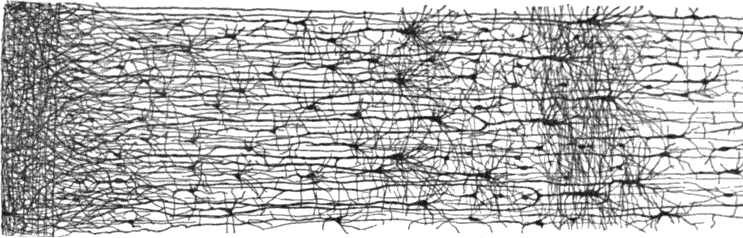
\includegraphics{brain}
    \caption{The brains structure under a microscope (cortex). Source:\cite{NN_book}}
    \labfig{brain}
\end{marginfigure}
\begin{marginfigure}
    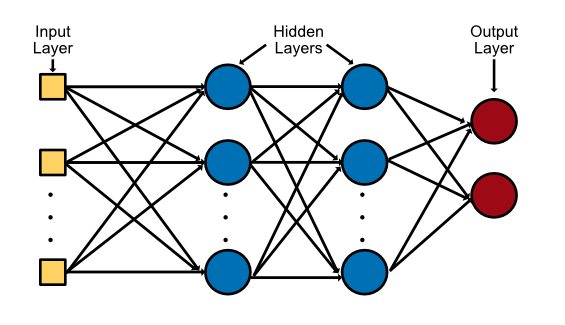
\includegraphics{MLP}
    \caption{Layers of an MLP.}
    \labfig{MLP}
\end{marginfigure}
Ultimately, MLPs really start to show the connected structure in a network that is typically expected.

MLPs are also called \textbf{fully connected networks} since each unit is connected to all unit in the previous layers as well as all units in the next layer.

%\marginnote{This new connectedness opens a realm to a whole field of studies on graphs, networks and network motifs \cite{network_motifs}.}

%histrocal rollercoaster of interest (AI winter) ?
%limited capabilities of the perceptron for XOR problem
%use either higher dimensional input -> kernel trick or stack many perceptrons
%any 2 layer MLP can approximate any continuous function (or somethign like that)
%simialrity to network motifs, make a large network of many identical pieces
%similar to how the brain works as well.

\subsubsection{Activation Functions}
%linear algebra shows that any linear function can approximated by just two perceptron layers for a linear activation function -> more layers do not make sense.
These newfound capabilities for MLPs are not only restricted to binary operations but will translate into continuous space.
In this case the hidden-layer perceptrons get stripped of their activation function.
The activation function of a perceptron has been used, up until now, to make a class prediction $y_i$ from a score $z_i$, which is also called pre-activation~\cite[p.~6]{grosse}.

Replacing the step function with a linear activation function (\eg identity function), each hidden-layer's perceptron would initially seem to increase the capabilities of the MLP.
Unfortunately, this is not the case as any subsequent perceptrons with linear activations can be reduced to a single preceptron.
\begin{align}
    \vec{z}_2 = \mat{W}^T_2 \vec{z}_1(\vec{x}) = \mat{W}^T_2 \mat{W}^T_1 \vec{x} = \mat{W}' \vec{x}
    \labeq{LAF}
\end{align}

Consequently, the step-function that was used in the \lstinline|XOR| problem played an important role.
The reason for this is the non-linear nature of the step-function in contrast to any linear activation function.
It can easily be shown that \refeq{LAF} does not hold if a non-linear activation function is used.

Thus, the question becomes which other activation functions there are that go beyond binary classification.
An early popular choice was sigmoid functions (logistic function or $\tanh$).
Especially the logistic function is popular due to its similarity to the step-function amongst other things.
\begin{align}
    \sigma(z) = \frac{1}{1 + e^{-z}}
\end{align}
\begin{marginfigure}
    \resizebox{\textwidth}{!}{
        %% Creator: Matplotlib, PGF backend
%%
%% To include the figure in your LaTeX document, write
%%   \input{<filename>.pgf}
%%
%% Make sure the required packages are loaded in your preamble
%%   \usepackage{pgf}
%%
%% and, on pdftex
%%   \usepackage[utf8]{inputenc}\DeclareUnicodeCharacter{2212}{-}
%%
%% or, on luatex and xetex
%%   \usepackage{unicode-math}
%%
%% Figures using additional raster images can only be included by \input if
%% they are in the same directory as the main LaTeX file. For loading figures
%% from other directories you can use the `import` package
%%   \usepackage{import}
%%
%% and then include the figures with
%%   \import{<path to file>}{<filename>.pgf}
%%
%% Matplotlib used the following preamble
%%
\begingroup%
\makeatletter%
\begin{pgfpicture}%
\pgfpathrectangle{\pgfpointorigin}{\pgfqpoint{10.000000in}{10.000000in}}%
\pgfusepath{use as bounding box, clip}%
\begin{pgfscope}%
\pgfsetbuttcap%
\pgfsetmiterjoin%
\definecolor{currentfill}{rgb}{1.000000,1.000000,1.000000}%
\pgfsetfillcolor{currentfill}%
\pgfsetlinewidth{0.000000pt}%
\definecolor{currentstroke}{rgb}{1.000000,1.000000,1.000000}%
\pgfsetstrokecolor{currentstroke}%
\pgfsetdash{}{0pt}%
\pgfpathmoveto{\pgfqpoint{0.000000in}{0.000000in}}%
\pgfpathlineto{\pgfqpoint{10.000000in}{0.000000in}}%
\pgfpathlineto{\pgfqpoint{10.000000in}{10.000000in}}%
\pgfpathlineto{\pgfqpoint{0.000000in}{10.000000in}}%
\pgfpathclose%
\pgfusepath{fill}%
\end{pgfscope}%
\begin{pgfscope}%
\pgfsetbuttcap%
\pgfsetmiterjoin%
\definecolor{currentfill}{rgb}{1.000000,1.000000,1.000000}%
\pgfsetfillcolor{currentfill}%
\pgfsetlinewidth{0.000000pt}%
\definecolor{currentstroke}{rgb}{0.000000,0.000000,0.000000}%
\pgfsetstrokecolor{currentstroke}%
\pgfsetstrokeopacity{0.000000}%
\pgfsetdash{}{0pt}%
\pgfpathmoveto{\pgfqpoint{1.250000in}{1.100000in}}%
\pgfpathlineto{\pgfqpoint{9.000000in}{1.100000in}}%
\pgfpathlineto{\pgfqpoint{9.000000in}{8.800000in}}%
\pgfpathlineto{\pgfqpoint{1.250000in}{8.800000in}}%
\pgfpathclose%
\pgfusepath{fill}%
\end{pgfscope}%
\begin{pgfscope}%
\pgfsetbuttcap%
\pgfsetroundjoin%
\definecolor{currentfill}{rgb}{0.000000,0.000000,0.000000}%
\pgfsetfillcolor{currentfill}%
\pgfsetlinewidth{0.803000pt}%
\definecolor{currentstroke}{rgb}{0.000000,0.000000,0.000000}%
\pgfsetstrokecolor{currentstroke}%
\pgfsetdash{}{0pt}%
\pgfsys@defobject{currentmarker}{\pgfqpoint{0.000000in}{-0.048611in}}{\pgfqpoint{0.000000in}{0.000000in}}{%
\pgfpathmoveto{\pgfqpoint{0.000000in}{0.000000in}}%
\pgfpathlineto{\pgfqpoint{0.000000in}{-0.048611in}}%
\pgfusepath{stroke,fill}%
}%
\begin{pgfscope}%
\pgfsys@transformshift{1.602273in}{1.100000in}%
\pgfsys@useobject{currentmarker}{}%
\end{pgfscope}%
\end{pgfscope}%
\begin{pgfscope}%
\definecolor{textcolor}{rgb}{0.000000,0.000000,0.000000}%
\pgfsetstrokecolor{textcolor}%
\pgfsetfillcolor{textcolor}%
\pgftext[x=1.602273in,y=1.002778in,,top]{\color{textcolor}\rmfamily\fontsize{10.000000}{12.000000}\selectfont \(\displaystyle -6\)}%
\end{pgfscope}%
\begin{pgfscope}%
\pgfsetbuttcap%
\pgfsetroundjoin%
\definecolor{currentfill}{rgb}{0.000000,0.000000,0.000000}%
\pgfsetfillcolor{currentfill}%
\pgfsetlinewidth{0.803000pt}%
\definecolor{currentstroke}{rgb}{0.000000,0.000000,0.000000}%
\pgfsetstrokecolor{currentstroke}%
\pgfsetdash{}{0pt}%
\pgfsys@defobject{currentmarker}{\pgfqpoint{0.000000in}{-0.048611in}}{\pgfqpoint{0.000000in}{0.000000in}}{%
\pgfpathmoveto{\pgfqpoint{0.000000in}{0.000000in}}%
\pgfpathlineto{\pgfqpoint{0.000000in}{-0.048611in}}%
\pgfusepath{stroke,fill}%
}%
\begin{pgfscope}%
\pgfsys@transformshift{2.777495in}{1.100000in}%
\pgfsys@useobject{currentmarker}{}%
\end{pgfscope}%
\end{pgfscope}%
\begin{pgfscope}%
\definecolor{textcolor}{rgb}{0.000000,0.000000,0.000000}%
\pgfsetstrokecolor{textcolor}%
\pgfsetfillcolor{textcolor}%
\pgftext[x=2.777495in,y=1.002778in,,top]{\color{textcolor}\rmfamily\fontsize{10.000000}{12.000000}\selectfont \(\displaystyle -4\)}%
\end{pgfscope}%
\begin{pgfscope}%
\pgfsetbuttcap%
\pgfsetroundjoin%
\definecolor{currentfill}{rgb}{0.000000,0.000000,0.000000}%
\pgfsetfillcolor{currentfill}%
\pgfsetlinewidth{0.803000pt}%
\definecolor{currentstroke}{rgb}{0.000000,0.000000,0.000000}%
\pgfsetstrokecolor{currentstroke}%
\pgfsetdash{}{0pt}%
\pgfsys@defobject{currentmarker}{\pgfqpoint{0.000000in}{-0.048611in}}{\pgfqpoint{0.000000in}{0.000000in}}{%
\pgfpathmoveto{\pgfqpoint{0.000000in}{0.000000in}}%
\pgfpathlineto{\pgfqpoint{0.000000in}{-0.048611in}}%
\pgfusepath{stroke,fill}%
}%
\begin{pgfscope}%
\pgfsys@transformshift{3.952716in}{1.100000in}%
\pgfsys@useobject{currentmarker}{}%
\end{pgfscope}%
\end{pgfscope}%
\begin{pgfscope}%
\definecolor{textcolor}{rgb}{0.000000,0.000000,0.000000}%
\pgfsetstrokecolor{textcolor}%
\pgfsetfillcolor{textcolor}%
\pgftext[x=3.952716in,y=1.002778in,,top]{\color{textcolor}\rmfamily\fontsize{10.000000}{12.000000}\selectfont \(\displaystyle -2\)}%
\end{pgfscope}%
\begin{pgfscope}%
\pgfsetbuttcap%
\pgfsetroundjoin%
\definecolor{currentfill}{rgb}{0.000000,0.000000,0.000000}%
\pgfsetfillcolor{currentfill}%
\pgfsetlinewidth{0.803000pt}%
\definecolor{currentstroke}{rgb}{0.000000,0.000000,0.000000}%
\pgfsetstrokecolor{currentstroke}%
\pgfsetdash{}{0pt}%
\pgfsys@defobject{currentmarker}{\pgfqpoint{0.000000in}{-0.048611in}}{\pgfqpoint{0.000000in}{0.000000in}}{%
\pgfpathmoveto{\pgfqpoint{0.000000in}{0.000000in}}%
\pgfpathlineto{\pgfqpoint{0.000000in}{-0.048611in}}%
\pgfusepath{stroke,fill}%
}%
\begin{pgfscope}%
\pgfsys@transformshift{5.127938in}{1.100000in}%
\pgfsys@useobject{currentmarker}{}%
\end{pgfscope}%
\end{pgfscope}%
\begin{pgfscope}%
\definecolor{textcolor}{rgb}{0.000000,0.000000,0.000000}%
\pgfsetstrokecolor{textcolor}%
\pgfsetfillcolor{textcolor}%
\pgftext[x=5.127938in,y=1.002778in,,top]{\color{textcolor}\rmfamily\fontsize{10.000000}{12.000000}\selectfont \(\displaystyle 0\)}%
\end{pgfscope}%
\begin{pgfscope}%
\pgfsetbuttcap%
\pgfsetroundjoin%
\definecolor{currentfill}{rgb}{0.000000,0.000000,0.000000}%
\pgfsetfillcolor{currentfill}%
\pgfsetlinewidth{0.803000pt}%
\definecolor{currentstroke}{rgb}{0.000000,0.000000,0.000000}%
\pgfsetstrokecolor{currentstroke}%
\pgfsetdash{}{0pt}%
\pgfsys@defobject{currentmarker}{\pgfqpoint{0.000000in}{-0.048611in}}{\pgfqpoint{0.000000in}{0.000000in}}{%
\pgfpathmoveto{\pgfqpoint{0.000000in}{0.000000in}}%
\pgfpathlineto{\pgfqpoint{0.000000in}{-0.048611in}}%
\pgfusepath{stroke,fill}%
}%
\begin{pgfscope}%
\pgfsys@transformshift{6.303160in}{1.100000in}%
\pgfsys@useobject{currentmarker}{}%
\end{pgfscope}%
\end{pgfscope}%
\begin{pgfscope}%
\definecolor{textcolor}{rgb}{0.000000,0.000000,0.000000}%
\pgfsetstrokecolor{textcolor}%
\pgfsetfillcolor{textcolor}%
\pgftext[x=6.303160in,y=1.002778in,,top]{\color{textcolor}\rmfamily\fontsize{10.000000}{12.000000}\selectfont \(\displaystyle 2\)}%
\end{pgfscope}%
\begin{pgfscope}%
\pgfsetbuttcap%
\pgfsetroundjoin%
\definecolor{currentfill}{rgb}{0.000000,0.000000,0.000000}%
\pgfsetfillcolor{currentfill}%
\pgfsetlinewidth{0.803000pt}%
\definecolor{currentstroke}{rgb}{0.000000,0.000000,0.000000}%
\pgfsetstrokecolor{currentstroke}%
\pgfsetdash{}{0pt}%
\pgfsys@defobject{currentmarker}{\pgfqpoint{0.000000in}{-0.048611in}}{\pgfqpoint{0.000000in}{0.000000in}}{%
\pgfpathmoveto{\pgfqpoint{0.000000in}{0.000000in}}%
\pgfpathlineto{\pgfqpoint{0.000000in}{-0.048611in}}%
\pgfusepath{stroke,fill}%
}%
\begin{pgfscope}%
\pgfsys@transformshift{7.478382in}{1.100000in}%
\pgfsys@useobject{currentmarker}{}%
\end{pgfscope}%
\end{pgfscope}%
\begin{pgfscope}%
\definecolor{textcolor}{rgb}{0.000000,0.000000,0.000000}%
\pgfsetstrokecolor{textcolor}%
\pgfsetfillcolor{textcolor}%
\pgftext[x=7.478382in,y=1.002778in,,top]{\color{textcolor}\rmfamily\fontsize{10.000000}{12.000000}\selectfont \(\displaystyle 4\)}%
\end{pgfscope}%
\begin{pgfscope}%
\pgfsetbuttcap%
\pgfsetroundjoin%
\definecolor{currentfill}{rgb}{0.000000,0.000000,0.000000}%
\pgfsetfillcolor{currentfill}%
\pgfsetlinewidth{0.803000pt}%
\definecolor{currentstroke}{rgb}{0.000000,0.000000,0.000000}%
\pgfsetstrokecolor{currentstroke}%
\pgfsetdash{}{0pt}%
\pgfsys@defobject{currentmarker}{\pgfqpoint{0.000000in}{-0.048611in}}{\pgfqpoint{0.000000in}{0.000000in}}{%
\pgfpathmoveto{\pgfqpoint{0.000000in}{0.000000in}}%
\pgfpathlineto{\pgfqpoint{0.000000in}{-0.048611in}}%
\pgfusepath{stroke,fill}%
}%
\begin{pgfscope}%
\pgfsys@transformshift{8.653603in}{1.100000in}%
\pgfsys@useobject{currentmarker}{}%
\end{pgfscope}%
\end{pgfscope}%
\begin{pgfscope}%
\definecolor{textcolor}{rgb}{0.000000,0.000000,0.000000}%
\pgfsetstrokecolor{textcolor}%
\pgfsetfillcolor{textcolor}%
\pgftext[x=8.653603in,y=1.002778in,,top]{\color{textcolor}\rmfamily\fontsize{10.000000}{12.000000}\selectfont \(\displaystyle 6\)}%
\end{pgfscope}%
\begin{pgfscope}%
\pgfsetbuttcap%
\pgfsetroundjoin%
\definecolor{currentfill}{rgb}{0.000000,0.000000,0.000000}%
\pgfsetfillcolor{currentfill}%
\pgfsetlinewidth{0.803000pt}%
\definecolor{currentstroke}{rgb}{0.000000,0.000000,0.000000}%
\pgfsetstrokecolor{currentstroke}%
\pgfsetdash{}{0pt}%
\pgfsys@defobject{currentmarker}{\pgfqpoint{-0.048611in}{0.000000in}}{\pgfqpoint{0.000000in}{0.000000in}}{%
\pgfpathmoveto{\pgfqpoint{0.000000in}{0.000000in}}%
\pgfpathlineto{\pgfqpoint{-0.048611in}{0.000000in}}%
\pgfusepath{stroke,fill}%
}%
\begin{pgfscope}%
\pgfsys@transformshift{1.250000in}{1.432605in}%
\pgfsys@useobject{currentmarker}{}%
\end{pgfscope}%
\end{pgfscope}%
\begin{pgfscope}%
\definecolor{textcolor}{rgb}{0.000000,0.000000,0.000000}%
\pgfsetstrokecolor{textcolor}%
\pgfsetfillcolor{textcolor}%
\pgftext[x=0.975308in, y=1.384380in, left, base]{\color{textcolor}\rmfamily\fontsize{10.000000}{12.000000}\selectfont \(\displaystyle 0.0\)}%
\end{pgfscope}%
\begin{pgfscope}%
\pgfsetbuttcap%
\pgfsetroundjoin%
\definecolor{currentfill}{rgb}{0.000000,0.000000,0.000000}%
\pgfsetfillcolor{currentfill}%
\pgfsetlinewidth{0.803000pt}%
\definecolor{currentstroke}{rgb}{0.000000,0.000000,0.000000}%
\pgfsetstrokecolor{currentstroke}%
\pgfsetdash{}{0pt}%
\pgfsys@defobject{currentmarker}{\pgfqpoint{-0.048611in}{0.000000in}}{\pgfqpoint{0.000000in}{0.000000in}}{%
\pgfpathmoveto{\pgfqpoint{0.000000in}{0.000000in}}%
\pgfpathlineto{\pgfqpoint{-0.048611in}{0.000000in}}%
\pgfusepath{stroke,fill}%
}%
\begin{pgfscope}%
\pgfsys@transformshift{1.250000in}{2.839598in}%
\pgfsys@useobject{currentmarker}{}%
\end{pgfscope}%
\end{pgfscope}%
\begin{pgfscope}%
\definecolor{textcolor}{rgb}{0.000000,0.000000,0.000000}%
\pgfsetstrokecolor{textcolor}%
\pgfsetfillcolor{textcolor}%
\pgftext[x=0.975308in, y=2.791373in, left, base]{\color{textcolor}\rmfamily\fontsize{10.000000}{12.000000}\selectfont \(\displaystyle 0.2\)}%
\end{pgfscope}%
\begin{pgfscope}%
\pgfsetbuttcap%
\pgfsetroundjoin%
\definecolor{currentfill}{rgb}{0.000000,0.000000,0.000000}%
\pgfsetfillcolor{currentfill}%
\pgfsetlinewidth{0.803000pt}%
\definecolor{currentstroke}{rgb}{0.000000,0.000000,0.000000}%
\pgfsetstrokecolor{currentstroke}%
\pgfsetdash{}{0pt}%
\pgfsys@defobject{currentmarker}{\pgfqpoint{-0.048611in}{0.000000in}}{\pgfqpoint{0.000000in}{0.000000in}}{%
\pgfpathmoveto{\pgfqpoint{0.000000in}{0.000000in}}%
\pgfpathlineto{\pgfqpoint{-0.048611in}{0.000000in}}%
\pgfusepath{stroke,fill}%
}%
\begin{pgfscope}%
\pgfsys@transformshift{1.250000in}{4.246591in}%
\pgfsys@useobject{currentmarker}{}%
\end{pgfscope}%
\end{pgfscope}%
\begin{pgfscope}%
\definecolor{textcolor}{rgb}{0.000000,0.000000,0.000000}%
\pgfsetstrokecolor{textcolor}%
\pgfsetfillcolor{textcolor}%
\pgftext[x=0.975308in, y=4.198366in, left, base]{\color{textcolor}\rmfamily\fontsize{10.000000}{12.000000}\selectfont \(\displaystyle 0.4\)}%
\end{pgfscope}%
\begin{pgfscope}%
\pgfsetbuttcap%
\pgfsetroundjoin%
\definecolor{currentfill}{rgb}{0.000000,0.000000,0.000000}%
\pgfsetfillcolor{currentfill}%
\pgfsetlinewidth{0.803000pt}%
\definecolor{currentstroke}{rgb}{0.000000,0.000000,0.000000}%
\pgfsetstrokecolor{currentstroke}%
\pgfsetdash{}{0pt}%
\pgfsys@defobject{currentmarker}{\pgfqpoint{-0.048611in}{0.000000in}}{\pgfqpoint{0.000000in}{0.000000in}}{%
\pgfpathmoveto{\pgfqpoint{0.000000in}{0.000000in}}%
\pgfpathlineto{\pgfqpoint{-0.048611in}{0.000000in}}%
\pgfusepath{stroke,fill}%
}%
\begin{pgfscope}%
\pgfsys@transformshift{1.250000in}{5.653584in}%
\pgfsys@useobject{currentmarker}{}%
\end{pgfscope}%
\end{pgfscope}%
\begin{pgfscope}%
\definecolor{textcolor}{rgb}{0.000000,0.000000,0.000000}%
\pgfsetstrokecolor{textcolor}%
\pgfsetfillcolor{textcolor}%
\pgftext[x=0.975308in, y=5.605358in, left, base]{\color{textcolor}\rmfamily\fontsize{10.000000}{12.000000}\selectfont \(\displaystyle 0.6\)}%
\end{pgfscope}%
\begin{pgfscope}%
\pgfsetbuttcap%
\pgfsetroundjoin%
\definecolor{currentfill}{rgb}{0.000000,0.000000,0.000000}%
\pgfsetfillcolor{currentfill}%
\pgfsetlinewidth{0.803000pt}%
\definecolor{currentstroke}{rgb}{0.000000,0.000000,0.000000}%
\pgfsetstrokecolor{currentstroke}%
\pgfsetdash{}{0pt}%
\pgfsys@defobject{currentmarker}{\pgfqpoint{-0.048611in}{0.000000in}}{\pgfqpoint{0.000000in}{0.000000in}}{%
\pgfpathmoveto{\pgfqpoint{0.000000in}{0.000000in}}%
\pgfpathlineto{\pgfqpoint{-0.048611in}{0.000000in}}%
\pgfusepath{stroke,fill}%
}%
\begin{pgfscope}%
\pgfsys@transformshift{1.250000in}{7.060576in}%
\pgfsys@useobject{currentmarker}{}%
\end{pgfscope}%
\end{pgfscope}%
\begin{pgfscope}%
\definecolor{textcolor}{rgb}{0.000000,0.000000,0.000000}%
\pgfsetstrokecolor{textcolor}%
\pgfsetfillcolor{textcolor}%
\pgftext[x=0.975308in, y=7.012351in, left, base]{\color{textcolor}\rmfamily\fontsize{10.000000}{12.000000}\selectfont \(\displaystyle 0.8\)}%
\end{pgfscope}%
\begin{pgfscope}%
\pgfsetbuttcap%
\pgfsetroundjoin%
\definecolor{currentfill}{rgb}{0.000000,0.000000,0.000000}%
\pgfsetfillcolor{currentfill}%
\pgfsetlinewidth{0.803000pt}%
\definecolor{currentstroke}{rgb}{0.000000,0.000000,0.000000}%
\pgfsetstrokecolor{currentstroke}%
\pgfsetdash{}{0pt}%
\pgfsys@defobject{currentmarker}{\pgfqpoint{-0.048611in}{0.000000in}}{\pgfqpoint{0.000000in}{0.000000in}}{%
\pgfpathmoveto{\pgfqpoint{0.000000in}{0.000000in}}%
\pgfpathlineto{\pgfqpoint{-0.048611in}{0.000000in}}%
\pgfusepath{stroke,fill}%
}%
\begin{pgfscope}%
\pgfsys@transformshift{1.250000in}{8.467569in}%
\pgfsys@useobject{currentmarker}{}%
\end{pgfscope}%
\end{pgfscope}%
\begin{pgfscope}%
\definecolor{textcolor}{rgb}{0.000000,0.000000,0.000000}%
\pgfsetstrokecolor{textcolor}%
\pgfsetfillcolor{textcolor}%
\pgftext[x=0.975308in, y=8.419344in, left, base]{\color{textcolor}\rmfamily\fontsize{10.000000}{12.000000}\selectfont \(\displaystyle 1.0\)}%
\end{pgfscope}%
\begin{pgfscope}%
\pgfpathrectangle{\pgfqpoint{1.250000in}{1.100000in}}{\pgfqpoint{7.750000in}{7.700000in}}%
\pgfusepath{clip}%
\pgfsetrectcap%
\pgfsetroundjoin%
\pgfsetlinewidth{2.007500pt}%
\definecolor{currentstroke}{rgb}{1.000000,0.000000,0.000000}%
\pgfsetstrokecolor{currentstroke}%
\pgfsetdash{}{0pt}%
\pgfpathmoveto{\pgfqpoint{1.602273in}{1.450000in}}%
\pgfpathlineto{\pgfqpoint{1.802060in}{1.457020in}}%
\pgfpathlineto{\pgfqpoint{1.972468in}{1.465195in}}%
\pgfpathlineto{\pgfqpoint{2.119370in}{1.474397in}}%
\pgfpathlineto{\pgfqpoint{2.248645in}{1.484604in}}%
\pgfpathlineto{\pgfqpoint{2.366167in}{1.496013in}}%
\pgfpathlineto{\pgfqpoint{2.471937in}{1.508384in}}%
\pgfpathlineto{\pgfqpoint{2.571831in}{1.522247in}}%
\pgfpathlineto{\pgfqpoint{2.665848in}{1.537569in}}%
\pgfpathlineto{\pgfqpoint{2.753990in}{1.554262in}}%
\pgfpathlineto{\pgfqpoint{2.836256in}{1.572181in}}%
\pgfpathlineto{\pgfqpoint{2.912645in}{1.591121in}}%
\pgfpathlineto{\pgfqpoint{2.983158in}{1.610820in}}%
\pgfpathlineto{\pgfqpoint{3.053672in}{1.632895in}}%
\pgfpathlineto{\pgfqpoint{3.118309in}{1.655446in}}%
\pgfpathlineto{\pgfqpoint{3.182946in}{1.680445in}}%
\pgfpathlineto{\pgfqpoint{3.241707in}{1.705499in}}%
\pgfpathlineto{\pgfqpoint{3.300468in}{1.732975in}}%
\pgfpathlineto{\pgfqpoint{3.359229in}{1.763081in}}%
\pgfpathlineto{\pgfqpoint{3.412114in}{1.792610in}}%
\pgfpathlineto{\pgfqpoint{3.464999in}{1.824624in}}%
\pgfpathlineto{\pgfqpoint{3.517884in}{1.859303in}}%
\pgfpathlineto{\pgfqpoint{3.570769in}{1.896835in}}%
\pgfpathlineto{\pgfqpoint{3.617778in}{1.932751in}}%
\pgfpathlineto{\pgfqpoint{3.664787in}{1.971217in}}%
\pgfpathlineto{\pgfqpoint{3.711796in}{2.012380in}}%
\pgfpathlineto{\pgfqpoint{3.758805in}{2.056386in}}%
\pgfpathlineto{\pgfqpoint{3.805814in}{2.103385in}}%
\pgfpathlineto{\pgfqpoint{3.852822in}{2.153527in}}%
\pgfpathlineto{\pgfqpoint{3.899831in}{2.206962in}}%
\pgfpathlineto{\pgfqpoint{3.946840in}{2.263835in}}%
\pgfpathlineto{\pgfqpoint{3.993849in}{2.324291in}}%
\pgfpathlineto{\pgfqpoint{4.040858in}{2.388466in}}%
\pgfpathlineto{\pgfqpoint{4.087867in}{2.456490in}}%
\pgfpathlineto{\pgfqpoint{4.134876in}{2.528483in}}%
\pgfpathlineto{\pgfqpoint{4.181885in}{2.604550in}}%
\pgfpathlineto{\pgfqpoint{4.228893in}{2.684784in}}%
\pgfpathlineto{\pgfqpoint{4.275902in}{2.769259in}}%
\pgfpathlineto{\pgfqpoint{4.322911in}{2.858029in}}%
\pgfpathlineto{\pgfqpoint{4.369920in}{2.951122in}}%
\pgfpathlineto{\pgfqpoint{4.422805in}{3.061025in}}%
\pgfpathlineto{\pgfqpoint{4.475690in}{3.176368in}}%
\pgfpathlineto{\pgfqpoint{4.528575in}{3.297063in}}%
\pgfpathlineto{\pgfqpoint{4.581460in}{3.422970in}}%
\pgfpathlineto{\pgfqpoint{4.640221in}{3.568737in}}%
\pgfpathlineto{\pgfqpoint{4.698982in}{3.720338in}}%
\pgfpathlineto{\pgfqpoint{4.763619in}{3.893305in}}%
\pgfpathlineto{\pgfqpoint{4.834133in}{4.088590in}}%
\pgfpathlineto{\pgfqpoint{4.910522in}{4.306677in}}%
\pgfpathlineto{\pgfqpoint{5.004540in}{4.582103in}}%
\pgfpathlineto{\pgfqpoint{5.157319in}{5.038006in}}%
\pgfpathlineto{\pgfqpoint{5.298345in}{5.456577in}}%
\pgfpathlineto{\pgfqpoint{5.386487in}{5.711686in}}%
\pgfpathlineto{\pgfqpoint{5.462876in}{5.926281in}}%
\pgfpathlineto{\pgfqpoint{5.533390in}{6.117659in}}%
\pgfpathlineto{\pgfqpoint{5.598027in}{6.286551in}}%
\pgfpathlineto{\pgfqpoint{5.656788in}{6.434109in}}%
\pgfpathlineto{\pgfqpoint{5.715549in}{6.575576in}}%
\pgfpathlineto{\pgfqpoint{5.768434in}{6.697444in}}%
\pgfpathlineto{\pgfqpoint{5.821319in}{6.813985in}}%
\pgfpathlineto{\pgfqpoint{5.874204in}{6.925102in}}%
\pgfpathlineto{\pgfqpoint{5.927089in}{7.030746in}}%
\pgfpathlineto{\pgfqpoint{5.974098in}{7.120055in}}%
\pgfpathlineto{\pgfqpoint{6.021107in}{7.205064in}}%
\pgfpathlineto{\pgfqpoint{6.068115in}{7.285825in}}%
\pgfpathlineto{\pgfqpoint{6.115124in}{7.362408in}}%
\pgfpathlineto{\pgfqpoint{6.162133in}{7.434904in}}%
\pgfpathlineto{\pgfqpoint{6.209142in}{7.503418in}}%
\pgfpathlineto{\pgfqpoint{6.256151in}{7.568068in}}%
\pgfpathlineto{\pgfqpoint{6.303160in}{7.628981in}}%
\pgfpathlineto{\pgfqpoint{6.350169in}{7.686294in}}%
\pgfpathlineto{\pgfqpoint{6.397178in}{7.740151in}}%
\pgfpathlineto{\pgfqpoint{6.444186in}{7.790696in}}%
\pgfpathlineto{\pgfqpoint{6.491195in}{7.838080in}}%
\pgfpathlineto{\pgfqpoint{6.538204in}{7.882452in}}%
\pgfpathlineto{\pgfqpoint{6.585213in}{7.923962in}}%
\pgfpathlineto{\pgfqpoint{6.632222in}{7.962757in}}%
\pgfpathlineto{\pgfqpoint{6.685107in}{8.003339in}}%
\pgfpathlineto{\pgfqpoint{6.737992in}{8.040871in}}%
\pgfpathlineto{\pgfqpoint{6.790877in}{8.075550in}}%
\pgfpathlineto{\pgfqpoint{6.843762in}{8.107564in}}%
\pgfpathlineto{\pgfqpoint{6.896647in}{8.137094in}}%
\pgfpathlineto{\pgfqpoint{6.955408in}{8.167200in}}%
\pgfpathlineto{\pgfqpoint{7.014169in}{8.194675in}}%
\pgfpathlineto{\pgfqpoint{7.072930in}{8.219729in}}%
\pgfpathlineto{\pgfqpoint{7.137567in}{8.244728in}}%
\pgfpathlineto{\pgfqpoint{7.202204in}{8.267280in}}%
\pgfpathlineto{\pgfqpoint{7.272718in}{8.289355in}}%
\pgfpathlineto{\pgfqpoint{7.343231in}{8.309053in}}%
\pgfpathlineto{\pgfqpoint{7.419621in}{8.327993in}}%
\pgfpathlineto{\pgfqpoint{7.496010in}{8.344711in}}%
\pgfpathlineto{\pgfqpoint{7.578275in}{8.360517in}}%
\pgfpathlineto{\pgfqpoint{7.666417in}{8.375233in}}%
\pgfpathlineto{\pgfqpoint{7.760435in}{8.388733in}}%
\pgfpathlineto{\pgfqpoint{7.866205in}{8.401597in}}%
\pgfpathlineto{\pgfqpoint{7.977851in}{8.412925in}}%
\pgfpathlineto{\pgfqpoint{8.101249in}{8.423210in}}%
\pgfpathlineto{\pgfqpoint{8.242276in}{8.432628in}}%
\pgfpathlineto{\pgfqpoint{8.400931in}{8.440864in}}%
\pgfpathlineto{\pgfqpoint{8.583090in}{8.447963in}}%
\pgfpathlineto{\pgfqpoint{8.647727in}{8.450000in}}%
\pgfpathlineto{\pgfqpoint{8.647727in}{8.450000in}}%
\pgfusepath{stroke}%
\end{pgfscope}%
\begin{pgfscope}%
\pgfsetrectcap%
\pgfsetmiterjoin%
\pgfsetlinewidth{0.803000pt}%
\definecolor{currentstroke}{rgb}{0.000000,0.000000,0.000000}%
\pgfsetstrokecolor{currentstroke}%
\pgfsetdash{}{0pt}%
\pgfpathmoveto{\pgfqpoint{1.250000in}{1.100000in}}%
\pgfpathlineto{\pgfqpoint{1.250000in}{8.800000in}}%
\pgfusepath{stroke}%
\end{pgfscope}%
\begin{pgfscope}%
\pgfsetrectcap%
\pgfsetmiterjoin%
\pgfsetlinewidth{0.803000pt}%
\definecolor{currentstroke}{rgb}{0.000000,0.000000,0.000000}%
\pgfsetstrokecolor{currentstroke}%
\pgfsetdash{}{0pt}%
\pgfpathmoveto{\pgfqpoint{9.000000in}{1.100000in}}%
\pgfpathlineto{\pgfqpoint{9.000000in}{8.800000in}}%
\pgfusepath{stroke}%
\end{pgfscope}%
\begin{pgfscope}%
\pgfsetrectcap%
\pgfsetmiterjoin%
\pgfsetlinewidth{0.803000pt}%
\definecolor{currentstroke}{rgb}{0.000000,0.000000,0.000000}%
\pgfsetstrokecolor{currentstroke}%
\pgfsetdash{}{0pt}%
\pgfpathmoveto{\pgfqpoint{1.250000in}{1.100000in}}%
\pgfpathlineto{\pgfqpoint{9.000000in}{1.100000in}}%
\pgfusepath{stroke}%
\end{pgfscope}%
\begin{pgfscope}%
\pgfsetrectcap%
\pgfsetmiterjoin%
\pgfsetlinewidth{0.803000pt}%
\definecolor{currentstroke}{rgb}{0.000000,0.000000,0.000000}%
\pgfsetstrokecolor{currentstroke}%
\pgfsetdash{}{0pt}%
\pgfpathmoveto{\pgfqpoint{1.250000in}{8.800000in}}%
\pgfpathlineto{\pgfqpoint{9.000000in}{8.800000in}}%
\pgfusepath{stroke}%
\end{pgfscope}%
\end{pgfpicture}%
\makeatother%
\endgroup%

    }
    \caption{A sigmoid function. It saturates to $1$ for very large inputs and $0$ for very small inputs, similar to the step function.}
    \labfig{sigmoid}
\end{marginfigure}

Another popular choice are rectified linear units (ReLU) which are identical to a linear activation for $z > 0$ but mimic the step function for $z < 0$.
Basically, a ReLU suppresses the signal of a perceptron until it reaches the threshold of $0$ and then forwards the signal unaltered.

Another activation function ``leaky ReLU'' attenuates the signal below the threshold with a factor $\alpha$ instead of fully suppressing it.
\begin{marginfigure}
    \resizebox{\textwidth}{!}{
        %% Creator: Matplotlib, PGF backend
%%
%% To include the figure in your LaTeX document, write
%%   \input{<filename>.pgf}
%%
%% Make sure the required packages are loaded in your preamble
%%   \usepackage{pgf}
%%
%% and, on pdftex
%%   \usepackage[utf8]{inputenc}\DeclareUnicodeCharacter{2212}{-}
%%
%% or, on luatex and xetex
%%   \usepackage{unicode-math}
%%
%% Figures using additional raster images can only be included by \input if
%% they are in the same directory as the main LaTeX file. For loading figures
%% from other directories you can use the `import` package
%%   \usepackage{import}
%%
%% and then include the figures with
%%   \import{<path to file>}{<filename>.pgf}
%%
%% Matplotlib used the following preamble
%%
\begingroup%
\makeatletter%
\begin{pgfpicture}%
\pgfpathrectangle{\pgfpointorigin}{\pgfqpoint{10.000000in}{10.000000in}}%
\pgfusepath{use as bounding box, clip}%
\begin{pgfscope}%
\pgfsetbuttcap%
\pgfsetmiterjoin%
\definecolor{currentfill}{rgb}{1.000000,1.000000,1.000000}%
\pgfsetfillcolor{currentfill}%
\pgfsetlinewidth{0.000000pt}%
\definecolor{currentstroke}{rgb}{1.000000,1.000000,1.000000}%
\pgfsetstrokecolor{currentstroke}%
\pgfsetdash{}{0pt}%
\pgfpathmoveto{\pgfqpoint{0.000000in}{0.000000in}}%
\pgfpathlineto{\pgfqpoint{10.000000in}{0.000000in}}%
\pgfpathlineto{\pgfqpoint{10.000000in}{10.000000in}}%
\pgfpathlineto{\pgfqpoint{0.000000in}{10.000000in}}%
\pgfpathclose%
\pgfusepath{fill}%
\end{pgfscope}%
\begin{pgfscope}%
\pgfsetbuttcap%
\pgfsetmiterjoin%
\definecolor{currentfill}{rgb}{1.000000,1.000000,1.000000}%
\pgfsetfillcolor{currentfill}%
\pgfsetlinewidth{0.000000pt}%
\definecolor{currentstroke}{rgb}{0.000000,0.000000,0.000000}%
\pgfsetstrokecolor{currentstroke}%
\pgfsetstrokeopacity{0.000000}%
\pgfsetdash{}{0pt}%
\pgfpathmoveto{\pgfqpoint{1.250000in}{1.100000in}}%
\pgfpathlineto{\pgfqpoint{9.000000in}{1.100000in}}%
\pgfpathlineto{\pgfqpoint{9.000000in}{8.800000in}}%
\pgfpathlineto{\pgfqpoint{1.250000in}{8.800000in}}%
\pgfpathclose%
\pgfusepath{fill}%
\end{pgfscope}%
\begin{pgfscope}%
\pgfsetbuttcap%
\pgfsetroundjoin%
\definecolor{currentfill}{rgb}{0.000000,0.000000,0.000000}%
\pgfsetfillcolor{currentfill}%
\pgfsetlinewidth{0.803000pt}%
\definecolor{currentstroke}{rgb}{0.000000,0.000000,0.000000}%
\pgfsetstrokecolor{currentstroke}%
\pgfsetdash{}{0pt}%
\pgfsys@defobject{currentmarker}{\pgfqpoint{0.000000in}{-0.048611in}}{\pgfqpoint{0.000000in}{0.000000in}}{%
\pgfpathmoveto{\pgfqpoint{0.000000in}{0.000000in}}%
\pgfpathlineto{\pgfqpoint{0.000000in}{-0.048611in}}%
\pgfusepath{stroke,fill}%
}%
\begin{pgfscope}%
\pgfsys@transformshift{1.602273in}{1.100000in}%
\pgfsys@useobject{currentmarker}{}%
\end{pgfscope}%
\end{pgfscope}%
\begin{pgfscope}%
\definecolor{textcolor}{rgb}{0.000000,0.000000,0.000000}%
\pgfsetstrokecolor{textcolor}%
\pgfsetfillcolor{textcolor}%
\pgftext[x=1.602273in,y=1.002778in,,top]{\color{textcolor}\rmfamily\fontsize{10.000000}{12.000000}\selectfont \(\displaystyle -6\)}%
\end{pgfscope}%
\begin{pgfscope}%
\pgfsetbuttcap%
\pgfsetroundjoin%
\definecolor{currentfill}{rgb}{0.000000,0.000000,0.000000}%
\pgfsetfillcolor{currentfill}%
\pgfsetlinewidth{0.803000pt}%
\definecolor{currentstroke}{rgb}{0.000000,0.000000,0.000000}%
\pgfsetstrokecolor{currentstroke}%
\pgfsetdash{}{0pt}%
\pgfsys@defobject{currentmarker}{\pgfqpoint{0.000000in}{-0.048611in}}{\pgfqpoint{0.000000in}{0.000000in}}{%
\pgfpathmoveto{\pgfqpoint{0.000000in}{0.000000in}}%
\pgfpathlineto{\pgfqpoint{0.000000in}{-0.048611in}}%
\pgfusepath{stroke,fill}%
}%
\begin{pgfscope}%
\pgfsys@transformshift{2.777495in}{1.100000in}%
\pgfsys@useobject{currentmarker}{}%
\end{pgfscope}%
\end{pgfscope}%
\begin{pgfscope}%
\definecolor{textcolor}{rgb}{0.000000,0.000000,0.000000}%
\pgfsetstrokecolor{textcolor}%
\pgfsetfillcolor{textcolor}%
\pgftext[x=2.777495in,y=1.002778in,,top]{\color{textcolor}\rmfamily\fontsize{10.000000}{12.000000}\selectfont \(\displaystyle -4\)}%
\end{pgfscope}%
\begin{pgfscope}%
\pgfsetbuttcap%
\pgfsetroundjoin%
\definecolor{currentfill}{rgb}{0.000000,0.000000,0.000000}%
\pgfsetfillcolor{currentfill}%
\pgfsetlinewidth{0.803000pt}%
\definecolor{currentstroke}{rgb}{0.000000,0.000000,0.000000}%
\pgfsetstrokecolor{currentstroke}%
\pgfsetdash{}{0pt}%
\pgfsys@defobject{currentmarker}{\pgfqpoint{0.000000in}{-0.048611in}}{\pgfqpoint{0.000000in}{0.000000in}}{%
\pgfpathmoveto{\pgfqpoint{0.000000in}{0.000000in}}%
\pgfpathlineto{\pgfqpoint{0.000000in}{-0.048611in}}%
\pgfusepath{stroke,fill}%
}%
\begin{pgfscope}%
\pgfsys@transformshift{3.952716in}{1.100000in}%
\pgfsys@useobject{currentmarker}{}%
\end{pgfscope}%
\end{pgfscope}%
\begin{pgfscope}%
\definecolor{textcolor}{rgb}{0.000000,0.000000,0.000000}%
\pgfsetstrokecolor{textcolor}%
\pgfsetfillcolor{textcolor}%
\pgftext[x=3.952716in,y=1.002778in,,top]{\color{textcolor}\rmfamily\fontsize{10.000000}{12.000000}\selectfont \(\displaystyle -2\)}%
\end{pgfscope}%
\begin{pgfscope}%
\pgfsetbuttcap%
\pgfsetroundjoin%
\definecolor{currentfill}{rgb}{0.000000,0.000000,0.000000}%
\pgfsetfillcolor{currentfill}%
\pgfsetlinewidth{0.803000pt}%
\definecolor{currentstroke}{rgb}{0.000000,0.000000,0.000000}%
\pgfsetstrokecolor{currentstroke}%
\pgfsetdash{}{0pt}%
\pgfsys@defobject{currentmarker}{\pgfqpoint{0.000000in}{-0.048611in}}{\pgfqpoint{0.000000in}{0.000000in}}{%
\pgfpathmoveto{\pgfqpoint{0.000000in}{0.000000in}}%
\pgfpathlineto{\pgfqpoint{0.000000in}{-0.048611in}}%
\pgfusepath{stroke,fill}%
}%
\begin{pgfscope}%
\pgfsys@transformshift{5.127938in}{1.100000in}%
\pgfsys@useobject{currentmarker}{}%
\end{pgfscope}%
\end{pgfscope}%
\begin{pgfscope}%
\definecolor{textcolor}{rgb}{0.000000,0.000000,0.000000}%
\pgfsetstrokecolor{textcolor}%
\pgfsetfillcolor{textcolor}%
\pgftext[x=5.127938in,y=1.002778in,,top]{\color{textcolor}\rmfamily\fontsize{10.000000}{12.000000}\selectfont \(\displaystyle 0\)}%
\end{pgfscope}%
\begin{pgfscope}%
\pgfsetbuttcap%
\pgfsetroundjoin%
\definecolor{currentfill}{rgb}{0.000000,0.000000,0.000000}%
\pgfsetfillcolor{currentfill}%
\pgfsetlinewidth{0.803000pt}%
\definecolor{currentstroke}{rgb}{0.000000,0.000000,0.000000}%
\pgfsetstrokecolor{currentstroke}%
\pgfsetdash{}{0pt}%
\pgfsys@defobject{currentmarker}{\pgfqpoint{0.000000in}{-0.048611in}}{\pgfqpoint{0.000000in}{0.000000in}}{%
\pgfpathmoveto{\pgfqpoint{0.000000in}{0.000000in}}%
\pgfpathlineto{\pgfqpoint{0.000000in}{-0.048611in}}%
\pgfusepath{stroke,fill}%
}%
\begin{pgfscope}%
\pgfsys@transformshift{6.303160in}{1.100000in}%
\pgfsys@useobject{currentmarker}{}%
\end{pgfscope}%
\end{pgfscope}%
\begin{pgfscope}%
\definecolor{textcolor}{rgb}{0.000000,0.000000,0.000000}%
\pgfsetstrokecolor{textcolor}%
\pgfsetfillcolor{textcolor}%
\pgftext[x=6.303160in,y=1.002778in,,top]{\color{textcolor}\rmfamily\fontsize{10.000000}{12.000000}\selectfont \(\displaystyle 2\)}%
\end{pgfscope}%
\begin{pgfscope}%
\pgfsetbuttcap%
\pgfsetroundjoin%
\definecolor{currentfill}{rgb}{0.000000,0.000000,0.000000}%
\pgfsetfillcolor{currentfill}%
\pgfsetlinewidth{0.803000pt}%
\definecolor{currentstroke}{rgb}{0.000000,0.000000,0.000000}%
\pgfsetstrokecolor{currentstroke}%
\pgfsetdash{}{0pt}%
\pgfsys@defobject{currentmarker}{\pgfqpoint{0.000000in}{-0.048611in}}{\pgfqpoint{0.000000in}{0.000000in}}{%
\pgfpathmoveto{\pgfqpoint{0.000000in}{0.000000in}}%
\pgfpathlineto{\pgfqpoint{0.000000in}{-0.048611in}}%
\pgfusepath{stroke,fill}%
}%
\begin{pgfscope}%
\pgfsys@transformshift{7.478382in}{1.100000in}%
\pgfsys@useobject{currentmarker}{}%
\end{pgfscope}%
\end{pgfscope}%
\begin{pgfscope}%
\definecolor{textcolor}{rgb}{0.000000,0.000000,0.000000}%
\pgfsetstrokecolor{textcolor}%
\pgfsetfillcolor{textcolor}%
\pgftext[x=7.478382in,y=1.002778in,,top]{\color{textcolor}\rmfamily\fontsize{10.000000}{12.000000}\selectfont \(\displaystyle 4\)}%
\end{pgfscope}%
\begin{pgfscope}%
\pgfsetbuttcap%
\pgfsetroundjoin%
\definecolor{currentfill}{rgb}{0.000000,0.000000,0.000000}%
\pgfsetfillcolor{currentfill}%
\pgfsetlinewidth{0.803000pt}%
\definecolor{currentstroke}{rgb}{0.000000,0.000000,0.000000}%
\pgfsetstrokecolor{currentstroke}%
\pgfsetdash{}{0pt}%
\pgfsys@defobject{currentmarker}{\pgfqpoint{0.000000in}{-0.048611in}}{\pgfqpoint{0.000000in}{0.000000in}}{%
\pgfpathmoveto{\pgfqpoint{0.000000in}{0.000000in}}%
\pgfpathlineto{\pgfqpoint{0.000000in}{-0.048611in}}%
\pgfusepath{stroke,fill}%
}%
\begin{pgfscope}%
\pgfsys@transformshift{8.653603in}{1.100000in}%
\pgfsys@useobject{currentmarker}{}%
\end{pgfscope}%
\end{pgfscope}%
\begin{pgfscope}%
\definecolor{textcolor}{rgb}{0.000000,0.000000,0.000000}%
\pgfsetstrokecolor{textcolor}%
\pgfsetfillcolor{textcolor}%
\pgftext[x=8.653603in,y=1.002778in,,top]{\color{textcolor}\rmfamily\fontsize{10.000000}{12.000000}\selectfont \(\displaystyle 6\)}%
\end{pgfscope}%
\begin{pgfscope}%
\pgfsetbuttcap%
\pgfsetroundjoin%
\definecolor{currentfill}{rgb}{0.000000,0.000000,0.000000}%
\pgfsetfillcolor{currentfill}%
\pgfsetlinewidth{0.803000pt}%
\definecolor{currentstroke}{rgb}{0.000000,0.000000,0.000000}%
\pgfsetstrokecolor{currentstroke}%
\pgfsetdash{}{0pt}%
\pgfsys@defobject{currentmarker}{\pgfqpoint{-0.048611in}{0.000000in}}{\pgfqpoint{0.000000in}{0.000000in}}{%
\pgfpathmoveto{\pgfqpoint{0.000000in}{0.000000in}}%
\pgfpathlineto{\pgfqpoint{-0.048611in}{0.000000in}}%
\pgfusepath{stroke,fill}%
}%
\begin{pgfscope}%
\pgfsys@transformshift{1.250000in}{1.450000in}%
\pgfsys@useobject{currentmarker}{}%
\end{pgfscope}%
\end{pgfscope}%
\begin{pgfscope}%
\definecolor{textcolor}{rgb}{0.000000,0.000000,0.000000}%
\pgfsetstrokecolor{textcolor}%
\pgfsetfillcolor{textcolor}%
\pgftext[x=1.083333in, y=1.401775in, left, base]{\color{textcolor}\rmfamily\fontsize{10.000000}{12.000000}\selectfont \(\displaystyle 0\)}%
\end{pgfscope}%
\begin{pgfscope}%
\pgfsetbuttcap%
\pgfsetroundjoin%
\definecolor{currentfill}{rgb}{0.000000,0.000000,0.000000}%
\pgfsetfillcolor{currentfill}%
\pgfsetlinewidth{0.803000pt}%
\definecolor{currentstroke}{rgb}{0.000000,0.000000,0.000000}%
\pgfsetstrokecolor{currentstroke}%
\pgfsetdash{}{0pt}%
\pgfsys@defobject{currentmarker}{\pgfqpoint{-0.048611in}{0.000000in}}{\pgfqpoint{0.000000in}{0.000000in}}{%
\pgfpathmoveto{\pgfqpoint{0.000000in}{0.000000in}}%
\pgfpathlineto{\pgfqpoint{-0.048611in}{0.000000in}}%
\pgfusepath{stroke,fill}%
}%
\begin{pgfscope}%
\pgfsys@transformshift{1.250000in}{2.618614in}%
\pgfsys@useobject{currentmarker}{}%
\end{pgfscope}%
\end{pgfscope}%
\begin{pgfscope}%
\definecolor{textcolor}{rgb}{0.000000,0.000000,0.000000}%
\pgfsetstrokecolor{textcolor}%
\pgfsetfillcolor{textcolor}%
\pgftext[x=1.083333in, y=2.570389in, left, base]{\color{textcolor}\rmfamily\fontsize{10.000000}{12.000000}\selectfont \(\displaystyle 1\)}%
\end{pgfscope}%
\begin{pgfscope}%
\pgfsetbuttcap%
\pgfsetroundjoin%
\definecolor{currentfill}{rgb}{0.000000,0.000000,0.000000}%
\pgfsetfillcolor{currentfill}%
\pgfsetlinewidth{0.803000pt}%
\definecolor{currentstroke}{rgb}{0.000000,0.000000,0.000000}%
\pgfsetstrokecolor{currentstroke}%
\pgfsetdash{}{0pt}%
\pgfsys@defobject{currentmarker}{\pgfqpoint{-0.048611in}{0.000000in}}{\pgfqpoint{0.000000in}{0.000000in}}{%
\pgfpathmoveto{\pgfqpoint{0.000000in}{0.000000in}}%
\pgfpathlineto{\pgfqpoint{-0.048611in}{0.000000in}}%
\pgfusepath{stroke,fill}%
}%
\begin{pgfscope}%
\pgfsys@transformshift{1.250000in}{3.787229in}%
\pgfsys@useobject{currentmarker}{}%
\end{pgfscope}%
\end{pgfscope}%
\begin{pgfscope}%
\definecolor{textcolor}{rgb}{0.000000,0.000000,0.000000}%
\pgfsetstrokecolor{textcolor}%
\pgfsetfillcolor{textcolor}%
\pgftext[x=1.083333in, y=3.739003in, left, base]{\color{textcolor}\rmfamily\fontsize{10.000000}{12.000000}\selectfont \(\displaystyle 2\)}%
\end{pgfscope}%
\begin{pgfscope}%
\pgfsetbuttcap%
\pgfsetroundjoin%
\definecolor{currentfill}{rgb}{0.000000,0.000000,0.000000}%
\pgfsetfillcolor{currentfill}%
\pgfsetlinewidth{0.803000pt}%
\definecolor{currentstroke}{rgb}{0.000000,0.000000,0.000000}%
\pgfsetstrokecolor{currentstroke}%
\pgfsetdash{}{0pt}%
\pgfsys@defobject{currentmarker}{\pgfqpoint{-0.048611in}{0.000000in}}{\pgfqpoint{0.000000in}{0.000000in}}{%
\pgfpathmoveto{\pgfqpoint{0.000000in}{0.000000in}}%
\pgfpathlineto{\pgfqpoint{-0.048611in}{0.000000in}}%
\pgfusepath{stroke,fill}%
}%
\begin{pgfscope}%
\pgfsys@transformshift{1.250000in}{4.955843in}%
\pgfsys@useobject{currentmarker}{}%
\end{pgfscope}%
\end{pgfscope}%
\begin{pgfscope}%
\definecolor{textcolor}{rgb}{0.000000,0.000000,0.000000}%
\pgfsetstrokecolor{textcolor}%
\pgfsetfillcolor{textcolor}%
\pgftext[x=1.083333in, y=4.907618in, left, base]{\color{textcolor}\rmfamily\fontsize{10.000000}{12.000000}\selectfont \(\displaystyle 3\)}%
\end{pgfscope}%
\begin{pgfscope}%
\pgfsetbuttcap%
\pgfsetroundjoin%
\definecolor{currentfill}{rgb}{0.000000,0.000000,0.000000}%
\pgfsetfillcolor{currentfill}%
\pgfsetlinewidth{0.803000pt}%
\definecolor{currentstroke}{rgb}{0.000000,0.000000,0.000000}%
\pgfsetstrokecolor{currentstroke}%
\pgfsetdash{}{0pt}%
\pgfsys@defobject{currentmarker}{\pgfqpoint{-0.048611in}{0.000000in}}{\pgfqpoint{0.000000in}{0.000000in}}{%
\pgfpathmoveto{\pgfqpoint{0.000000in}{0.000000in}}%
\pgfpathlineto{\pgfqpoint{-0.048611in}{0.000000in}}%
\pgfusepath{stroke,fill}%
}%
\begin{pgfscope}%
\pgfsys@transformshift{1.250000in}{6.124457in}%
\pgfsys@useobject{currentmarker}{}%
\end{pgfscope}%
\end{pgfscope}%
\begin{pgfscope}%
\definecolor{textcolor}{rgb}{0.000000,0.000000,0.000000}%
\pgfsetstrokecolor{textcolor}%
\pgfsetfillcolor{textcolor}%
\pgftext[x=1.083333in, y=6.076232in, left, base]{\color{textcolor}\rmfamily\fontsize{10.000000}{12.000000}\selectfont \(\displaystyle 4\)}%
\end{pgfscope}%
\begin{pgfscope}%
\pgfsetbuttcap%
\pgfsetroundjoin%
\definecolor{currentfill}{rgb}{0.000000,0.000000,0.000000}%
\pgfsetfillcolor{currentfill}%
\pgfsetlinewidth{0.803000pt}%
\definecolor{currentstroke}{rgb}{0.000000,0.000000,0.000000}%
\pgfsetstrokecolor{currentstroke}%
\pgfsetdash{}{0pt}%
\pgfsys@defobject{currentmarker}{\pgfqpoint{-0.048611in}{0.000000in}}{\pgfqpoint{0.000000in}{0.000000in}}{%
\pgfpathmoveto{\pgfqpoint{0.000000in}{0.000000in}}%
\pgfpathlineto{\pgfqpoint{-0.048611in}{0.000000in}}%
\pgfusepath{stroke,fill}%
}%
\begin{pgfscope}%
\pgfsys@transformshift{1.250000in}{7.293072in}%
\pgfsys@useobject{currentmarker}{}%
\end{pgfscope}%
\end{pgfscope}%
\begin{pgfscope}%
\definecolor{textcolor}{rgb}{0.000000,0.000000,0.000000}%
\pgfsetstrokecolor{textcolor}%
\pgfsetfillcolor{textcolor}%
\pgftext[x=1.083333in, y=7.244847in, left, base]{\color{textcolor}\rmfamily\fontsize{10.000000}{12.000000}\selectfont \(\displaystyle 5\)}%
\end{pgfscope}%
\begin{pgfscope}%
\pgfsetbuttcap%
\pgfsetroundjoin%
\definecolor{currentfill}{rgb}{0.000000,0.000000,0.000000}%
\pgfsetfillcolor{currentfill}%
\pgfsetlinewidth{0.803000pt}%
\definecolor{currentstroke}{rgb}{0.000000,0.000000,0.000000}%
\pgfsetstrokecolor{currentstroke}%
\pgfsetdash{}{0pt}%
\pgfsys@defobject{currentmarker}{\pgfqpoint{-0.048611in}{0.000000in}}{\pgfqpoint{0.000000in}{0.000000in}}{%
\pgfpathmoveto{\pgfqpoint{0.000000in}{0.000000in}}%
\pgfpathlineto{\pgfqpoint{-0.048611in}{0.000000in}}%
\pgfusepath{stroke,fill}%
}%
\begin{pgfscope}%
\pgfsys@transformshift{1.250000in}{8.461686in}%
\pgfsys@useobject{currentmarker}{}%
\end{pgfscope}%
\end{pgfscope}%
\begin{pgfscope}%
\definecolor{textcolor}{rgb}{0.000000,0.000000,0.000000}%
\pgfsetstrokecolor{textcolor}%
\pgfsetfillcolor{textcolor}%
\pgftext[x=1.083333in, y=8.413461in, left, base]{\color{textcolor}\rmfamily\fontsize{10.000000}{12.000000}\selectfont \(\displaystyle 6\)}%
\end{pgfscope}%
\begin{pgfscope}%
\pgfpathrectangle{\pgfqpoint{1.250000in}{1.100000in}}{\pgfqpoint{7.750000in}{7.700000in}}%
\pgfusepath{clip}%
\pgfsetrectcap%
\pgfsetroundjoin%
\pgfsetlinewidth{2.007500pt}%
\definecolor{currentstroke}{rgb}{1.000000,0.000000,0.000000}%
\pgfsetstrokecolor{currentstroke}%
\pgfsetdash{}{0pt}%
\pgfpathmoveto{\pgfqpoint{1.602273in}{1.450000in}}%
\pgfpathlineto{\pgfqpoint{5.127938in}{1.450000in}}%
\pgfpathlineto{\pgfqpoint{8.647727in}{8.450000in}}%
\pgfpathlineto{\pgfqpoint{8.647727in}{8.450000in}}%
\pgfusepath{stroke}%
\end{pgfscope}%
\begin{pgfscope}%
\pgfsetrectcap%
\pgfsetmiterjoin%
\pgfsetlinewidth{0.803000pt}%
\definecolor{currentstroke}{rgb}{0.000000,0.000000,0.000000}%
\pgfsetstrokecolor{currentstroke}%
\pgfsetdash{}{0pt}%
\pgfpathmoveto{\pgfqpoint{1.250000in}{1.100000in}}%
\pgfpathlineto{\pgfqpoint{1.250000in}{8.800000in}}%
\pgfusepath{stroke}%
\end{pgfscope}%
\begin{pgfscope}%
\pgfsetrectcap%
\pgfsetmiterjoin%
\pgfsetlinewidth{0.803000pt}%
\definecolor{currentstroke}{rgb}{0.000000,0.000000,0.000000}%
\pgfsetstrokecolor{currentstroke}%
\pgfsetdash{}{0pt}%
\pgfpathmoveto{\pgfqpoint{9.000000in}{1.100000in}}%
\pgfpathlineto{\pgfqpoint{9.000000in}{8.800000in}}%
\pgfusepath{stroke}%
\end{pgfscope}%
\begin{pgfscope}%
\pgfsetrectcap%
\pgfsetmiterjoin%
\pgfsetlinewidth{0.803000pt}%
\definecolor{currentstroke}{rgb}{0.000000,0.000000,0.000000}%
\pgfsetstrokecolor{currentstroke}%
\pgfsetdash{}{0pt}%
\pgfpathmoveto{\pgfqpoint{1.250000in}{1.100000in}}%
\pgfpathlineto{\pgfqpoint{9.000000in}{1.100000in}}%
\pgfusepath{stroke}%
\end{pgfscope}%
\begin{pgfscope}%
\pgfsetrectcap%
\pgfsetmiterjoin%
\pgfsetlinewidth{0.803000pt}%
\definecolor{currentstroke}{rgb}{0.000000,0.000000,0.000000}%
\pgfsetstrokecolor{currentstroke}%
\pgfsetdash{}{0pt}%
\pgfpathmoveto{\pgfqpoint{1.250000in}{8.800000in}}%
\pgfpathlineto{\pgfqpoint{9.000000in}{8.800000in}}%
\pgfusepath{stroke}%
\end{pgfscope}%
\end{pgfpicture}%
\makeatother%
\endgroup%

    }
    \caption{ReLu activation function}
    \labfig{relu}
\end{marginfigure}
\begin{marginfigure}
    \resizebox{\textwidth}{!}{
        %% Creator: Matplotlib, PGF backend
%%
%% To include the figure in your LaTeX document, write
%%   \input{<filename>.pgf}
%%
%% Make sure the required packages are loaded in your preamble
%%   \usepackage{pgf}
%%
%% and, on pdftex
%%   \usepackage[utf8]{inputenc}\DeclareUnicodeCharacter{2212}{-}
%%
%% or, on luatex and xetex
%%   \usepackage{unicode-math}
%%
%% Figures using additional raster images can only be included by \input if
%% they are in the same directory as the main LaTeX file. For loading figures
%% from other directories you can use the `import` package
%%   \usepackage{import}
%%
%% and then include the figures with
%%   \import{<path to file>}{<filename>.pgf}
%%
%% Matplotlib used the following preamble
%%
\begingroup%
\makeatletter%
\begin{pgfpicture}%
\pgfpathrectangle{\pgfpointorigin}{\pgfqpoint{10.000000in}{10.000000in}}%
\pgfusepath{use as bounding box, clip}%
\begin{pgfscope}%
\pgfsetbuttcap%
\pgfsetmiterjoin%
\definecolor{currentfill}{rgb}{1.000000,1.000000,1.000000}%
\pgfsetfillcolor{currentfill}%
\pgfsetlinewidth{0.000000pt}%
\definecolor{currentstroke}{rgb}{1.000000,1.000000,1.000000}%
\pgfsetstrokecolor{currentstroke}%
\pgfsetdash{}{0pt}%
\pgfpathmoveto{\pgfqpoint{0.000000in}{0.000000in}}%
\pgfpathlineto{\pgfqpoint{10.000000in}{0.000000in}}%
\pgfpathlineto{\pgfqpoint{10.000000in}{10.000000in}}%
\pgfpathlineto{\pgfqpoint{0.000000in}{10.000000in}}%
\pgfpathclose%
\pgfusepath{fill}%
\end{pgfscope}%
\begin{pgfscope}%
\pgfsetbuttcap%
\pgfsetmiterjoin%
\definecolor{currentfill}{rgb}{1.000000,1.000000,1.000000}%
\pgfsetfillcolor{currentfill}%
\pgfsetlinewidth{0.000000pt}%
\definecolor{currentstroke}{rgb}{0.000000,0.000000,0.000000}%
\pgfsetstrokecolor{currentstroke}%
\pgfsetstrokeopacity{0.000000}%
\pgfsetdash{}{0pt}%
\pgfpathmoveto{\pgfqpoint{1.250000in}{1.100000in}}%
\pgfpathlineto{\pgfqpoint{9.000000in}{1.100000in}}%
\pgfpathlineto{\pgfqpoint{9.000000in}{8.800000in}}%
\pgfpathlineto{\pgfqpoint{1.250000in}{8.800000in}}%
\pgfpathclose%
\pgfusepath{fill}%
\end{pgfscope}%
\begin{pgfscope}%
\pgfsetbuttcap%
\pgfsetroundjoin%
\definecolor{currentfill}{rgb}{0.000000,0.000000,0.000000}%
\pgfsetfillcolor{currentfill}%
\pgfsetlinewidth{0.803000pt}%
\definecolor{currentstroke}{rgb}{0.000000,0.000000,0.000000}%
\pgfsetstrokecolor{currentstroke}%
\pgfsetdash{}{0pt}%
\pgfsys@defobject{currentmarker}{\pgfqpoint{0.000000in}{-0.048611in}}{\pgfqpoint{0.000000in}{0.000000in}}{%
\pgfpathmoveto{\pgfqpoint{0.000000in}{0.000000in}}%
\pgfpathlineto{\pgfqpoint{0.000000in}{-0.048611in}}%
\pgfusepath{stroke,fill}%
}%
\begin{pgfscope}%
\pgfsys@transformshift{1.602273in}{1.100000in}%
\pgfsys@useobject{currentmarker}{}%
\end{pgfscope}%
\end{pgfscope}%
\begin{pgfscope}%
\definecolor{textcolor}{rgb}{0.000000,0.000000,0.000000}%
\pgfsetstrokecolor{textcolor}%
\pgfsetfillcolor{textcolor}%
\pgftext[x=1.602273in,y=1.002778in,,top]{\color{textcolor}\rmfamily\fontsize{10.000000}{12.000000}\selectfont \(\displaystyle -6\)}%
\end{pgfscope}%
\begin{pgfscope}%
\pgfsetbuttcap%
\pgfsetroundjoin%
\definecolor{currentfill}{rgb}{0.000000,0.000000,0.000000}%
\pgfsetfillcolor{currentfill}%
\pgfsetlinewidth{0.803000pt}%
\definecolor{currentstroke}{rgb}{0.000000,0.000000,0.000000}%
\pgfsetstrokecolor{currentstroke}%
\pgfsetdash{}{0pt}%
\pgfsys@defobject{currentmarker}{\pgfqpoint{0.000000in}{-0.048611in}}{\pgfqpoint{0.000000in}{0.000000in}}{%
\pgfpathmoveto{\pgfqpoint{0.000000in}{0.000000in}}%
\pgfpathlineto{\pgfqpoint{0.000000in}{-0.048611in}}%
\pgfusepath{stroke,fill}%
}%
\begin{pgfscope}%
\pgfsys@transformshift{2.777495in}{1.100000in}%
\pgfsys@useobject{currentmarker}{}%
\end{pgfscope}%
\end{pgfscope}%
\begin{pgfscope}%
\definecolor{textcolor}{rgb}{0.000000,0.000000,0.000000}%
\pgfsetstrokecolor{textcolor}%
\pgfsetfillcolor{textcolor}%
\pgftext[x=2.777495in,y=1.002778in,,top]{\color{textcolor}\rmfamily\fontsize{10.000000}{12.000000}\selectfont \(\displaystyle -4\)}%
\end{pgfscope}%
\begin{pgfscope}%
\pgfsetbuttcap%
\pgfsetroundjoin%
\definecolor{currentfill}{rgb}{0.000000,0.000000,0.000000}%
\pgfsetfillcolor{currentfill}%
\pgfsetlinewidth{0.803000pt}%
\definecolor{currentstroke}{rgb}{0.000000,0.000000,0.000000}%
\pgfsetstrokecolor{currentstroke}%
\pgfsetdash{}{0pt}%
\pgfsys@defobject{currentmarker}{\pgfqpoint{0.000000in}{-0.048611in}}{\pgfqpoint{0.000000in}{0.000000in}}{%
\pgfpathmoveto{\pgfqpoint{0.000000in}{0.000000in}}%
\pgfpathlineto{\pgfqpoint{0.000000in}{-0.048611in}}%
\pgfusepath{stroke,fill}%
}%
\begin{pgfscope}%
\pgfsys@transformshift{3.952716in}{1.100000in}%
\pgfsys@useobject{currentmarker}{}%
\end{pgfscope}%
\end{pgfscope}%
\begin{pgfscope}%
\definecolor{textcolor}{rgb}{0.000000,0.000000,0.000000}%
\pgfsetstrokecolor{textcolor}%
\pgfsetfillcolor{textcolor}%
\pgftext[x=3.952716in,y=1.002778in,,top]{\color{textcolor}\rmfamily\fontsize{10.000000}{12.000000}\selectfont \(\displaystyle -2\)}%
\end{pgfscope}%
\begin{pgfscope}%
\pgfsetbuttcap%
\pgfsetroundjoin%
\definecolor{currentfill}{rgb}{0.000000,0.000000,0.000000}%
\pgfsetfillcolor{currentfill}%
\pgfsetlinewidth{0.803000pt}%
\definecolor{currentstroke}{rgb}{0.000000,0.000000,0.000000}%
\pgfsetstrokecolor{currentstroke}%
\pgfsetdash{}{0pt}%
\pgfsys@defobject{currentmarker}{\pgfqpoint{0.000000in}{-0.048611in}}{\pgfqpoint{0.000000in}{0.000000in}}{%
\pgfpathmoveto{\pgfqpoint{0.000000in}{0.000000in}}%
\pgfpathlineto{\pgfqpoint{0.000000in}{-0.048611in}}%
\pgfusepath{stroke,fill}%
}%
\begin{pgfscope}%
\pgfsys@transformshift{5.127938in}{1.100000in}%
\pgfsys@useobject{currentmarker}{}%
\end{pgfscope}%
\end{pgfscope}%
\begin{pgfscope}%
\definecolor{textcolor}{rgb}{0.000000,0.000000,0.000000}%
\pgfsetstrokecolor{textcolor}%
\pgfsetfillcolor{textcolor}%
\pgftext[x=5.127938in,y=1.002778in,,top]{\color{textcolor}\rmfamily\fontsize{10.000000}{12.000000}\selectfont \(\displaystyle 0\)}%
\end{pgfscope}%
\begin{pgfscope}%
\pgfsetbuttcap%
\pgfsetroundjoin%
\definecolor{currentfill}{rgb}{0.000000,0.000000,0.000000}%
\pgfsetfillcolor{currentfill}%
\pgfsetlinewidth{0.803000pt}%
\definecolor{currentstroke}{rgb}{0.000000,0.000000,0.000000}%
\pgfsetstrokecolor{currentstroke}%
\pgfsetdash{}{0pt}%
\pgfsys@defobject{currentmarker}{\pgfqpoint{0.000000in}{-0.048611in}}{\pgfqpoint{0.000000in}{0.000000in}}{%
\pgfpathmoveto{\pgfqpoint{0.000000in}{0.000000in}}%
\pgfpathlineto{\pgfqpoint{0.000000in}{-0.048611in}}%
\pgfusepath{stroke,fill}%
}%
\begin{pgfscope}%
\pgfsys@transformshift{6.303160in}{1.100000in}%
\pgfsys@useobject{currentmarker}{}%
\end{pgfscope}%
\end{pgfscope}%
\begin{pgfscope}%
\definecolor{textcolor}{rgb}{0.000000,0.000000,0.000000}%
\pgfsetstrokecolor{textcolor}%
\pgfsetfillcolor{textcolor}%
\pgftext[x=6.303160in,y=1.002778in,,top]{\color{textcolor}\rmfamily\fontsize{10.000000}{12.000000}\selectfont \(\displaystyle 2\)}%
\end{pgfscope}%
\begin{pgfscope}%
\pgfsetbuttcap%
\pgfsetroundjoin%
\definecolor{currentfill}{rgb}{0.000000,0.000000,0.000000}%
\pgfsetfillcolor{currentfill}%
\pgfsetlinewidth{0.803000pt}%
\definecolor{currentstroke}{rgb}{0.000000,0.000000,0.000000}%
\pgfsetstrokecolor{currentstroke}%
\pgfsetdash{}{0pt}%
\pgfsys@defobject{currentmarker}{\pgfqpoint{0.000000in}{-0.048611in}}{\pgfqpoint{0.000000in}{0.000000in}}{%
\pgfpathmoveto{\pgfqpoint{0.000000in}{0.000000in}}%
\pgfpathlineto{\pgfqpoint{0.000000in}{-0.048611in}}%
\pgfusepath{stroke,fill}%
}%
\begin{pgfscope}%
\pgfsys@transformshift{7.478382in}{1.100000in}%
\pgfsys@useobject{currentmarker}{}%
\end{pgfscope}%
\end{pgfscope}%
\begin{pgfscope}%
\definecolor{textcolor}{rgb}{0.000000,0.000000,0.000000}%
\pgfsetstrokecolor{textcolor}%
\pgfsetfillcolor{textcolor}%
\pgftext[x=7.478382in,y=1.002778in,,top]{\color{textcolor}\rmfamily\fontsize{10.000000}{12.000000}\selectfont \(\displaystyle 4\)}%
\end{pgfscope}%
\begin{pgfscope}%
\pgfsetbuttcap%
\pgfsetroundjoin%
\definecolor{currentfill}{rgb}{0.000000,0.000000,0.000000}%
\pgfsetfillcolor{currentfill}%
\pgfsetlinewidth{0.803000pt}%
\definecolor{currentstroke}{rgb}{0.000000,0.000000,0.000000}%
\pgfsetstrokecolor{currentstroke}%
\pgfsetdash{}{0pt}%
\pgfsys@defobject{currentmarker}{\pgfqpoint{0.000000in}{-0.048611in}}{\pgfqpoint{0.000000in}{0.000000in}}{%
\pgfpathmoveto{\pgfqpoint{0.000000in}{0.000000in}}%
\pgfpathlineto{\pgfqpoint{0.000000in}{-0.048611in}}%
\pgfusepath{stroke,fill}%
}%
\begin{pgfscope}%
\pgfsys@transformshift{8.653603in}{1.100000in}%
\pgfsys@useobject{currentmarker}{}%
\end{pgfscope}%
\end{pgfscope}%
\begin{pgfscope}%
\definecolor{textcolor}{rgb}{0.000000,0.000000,0.000000}%
\pgfsetstrokecolor{textcolor}%
\pgfsetfillcolor{textcolor}%
\pgftext[x=8.653603in,y=1.002778in,,top]{\color{textcolor}\rmfamily\fontsize{10.000000}{12.000000}\selectfont \(\displaystyle 6\)}%
\end{pgfscope}%
\begin{pgfscope}%
\pgfsetbuttcap%
\pgfsetroundjoin%
\definecolor{currentfill}{rgb}{0.000000,0.000000,0.000000}%
\pgfsetfillcolor{currentfill}%
\pgfsetlinewidth{0.803000pt}%
\definecolor{currentstroke}{rgb}{0.000000,0.000000,0.000000}%
\pgfsetstrokecolor{currentstroke}%
\pgfsetdash{}{0pt}%
\pgfsys@defobject{currentmarker}{\pgfqpoint{-0.048611in}{0.000000in}}{\pgfqpoint{0.000000in}{0.000000in}}{%
\pgfpathmoveto{\pgfqpoint{0.000000in}{0.000000in}}%
\pgfpathlineto{\pgfqpoint{-0.048611in}{0.000000in}}%
\pgfusepath{stroke,fill}%
}%
\begin{pgfscope}%
\pgfsys@transformshift{1.250000in}{1.644715in}%
\pgfsys@useobject{currentmarker}{}%
\end{pgfscope}%
\end{pgfscope}%
\begin{pgfscope}%
\definecolor{textcolor}{rgb}{0.000000,0.000000,0.000000}%
\pgfsetstrokecolor{textcolor}%
\pgfsetfillcolor{textcolor}%
\pgftext[x=0.975308in, y=1.596490in, left, base]{\color{textcolor}\rmfamily\fontsize{10.000000}{12.000000}\selectfont \(\displaystyle -1\)}%
\end{pgfscope}%
\begin{pgfscope}%
\pgfsetbuttcap%
\pgfsetroundjoin%
\definecolor{currentfill}{rgb}{0.000000,0.000000,0.000000}%
\pgfsetfillcolor{currentfill}%
\pgfsetlinewidth{0.803000pt}%
\definecolor{currentstroke}{rgb}{0.000000,0.000000,0.000000}%
\pgfsetstrokecolor{currentstroke}%
\pgfsetdash{}{0pt}%
\pgfsys@defobject{currentmarker}{\pgfqpoint{-0.048611in}{0.000000in}}{\pgfqpoint{0.000000in}{0.000000in}}{%
\pgfpathmoveto{\pgfqpoint{0.000000in}{0.000000in}}%
\pgfpathlineto{\pgfqpoint{-0.048611in}{0.000000in}}%
\pgfusepath{stroke,fill}%
}%
\begin{pgfscope}%
\pgfsys@transformshift{1.250000in}{2.618289in}%
\pgfsys@useobject{currentmarker}{}%
\end{pgfscope}%
\end{pgfscope}%
\begin{pgfscope}%
\definecolor{textcolor}{rgb}{0.000000,0.000000,0.000000}%
\pgfsetstrokecolor{textcolor}%
\pgfsetfillcolor{textcolor}%
\pgftext[x=1.083333in, y=2.570064in, left, base]{\color{textcolor}\rmfamily\fontsize{10.000000}{12.000000}\selectfont \(\displaystyle 0\)}%
\end{pgfscope}%
\begin{pgfscope}%
\pgfsetbuttcap%
\pgfsetroundjoin%
\definecolor{currentfill}{rgb}{0.000000,0.000000,0.000000}%
\pgfsetfillcolor{currentfill}%
\pgfsetlinewidth{0.803000pt}%
\definecolor{currentstroke}{rgb}{0.000000,0.000000,0.000000}%
\pgfsetstrokecolor{currentstroke}%
\pgfsetdash{}{0pt}%
\pgfsys@defobject{currentmarker}{\pgfqpoint{-0.048611in}{0.000000in}}{\pgfqpoint{0.000000in}{0.000000in}}{%
\pgfpathmoveto{\pgfqpoint{0.000000in}{0.000000in}}%
\pgfpathlineto{\pgfqpoint{-0.048611in}{0.000000in}}%
\pgfusepath{stroke,fill}%
}%
\begin{pgfscope}%
\pgfsys@transformshift{1.250000in}{3.591864in}%
\pgfsys@useobject{currentmarker}{}%
\end{pgfscope}%
\end{pgfscope}%
\begin{pgfscope}%
\definecolor{textcolor}{rgb}{0.000000,0.000000,0.000000}%
\pgfsetstrokecolor{textcolor}%
\pgfsetfillcolor{textcolor}%
\pgftext[x=1.083333in, y=3.543638in, left, base]{\color{textcolor}\rmfamily\fontsize{10.000000}{12.000000}\selectfont \(\displaystyle 1\)}%
\end{pgfscope}%
\begin{pgfscope}%
\pgfsetbuttcap%
\pgfsetroundjoin%
\definecolor{currentfill}{rgb}{0.000000,0.000000,0.000000}%
\pgfsetfillcolor{currentfill}%
\pgfsetlinewidth{0.803000pt}%
\definecolor{currentstroke}{rgb}{0.000000,0.000000,0.000000}%
\pgfsetstrokecolor{currentstroke}%
\pgfsetdash{}{0pt}%
\pgfsys@defobject{currentmarker}{\pgfqpoint{-0.048611in}{0.000000in}}{\pgfqpoint{0.000000in}{0.000000in}}{%
\pgfpathmoveto{\pgfqpoint{0.000000in}{0.000000in}}%
\pgfpathlineto{\pgfqpoint{-0.048611in}{0.000000in}}%
\pgfusepath{stroke,fill}%
}%
\begin{pgfscope}%
\pgfsys@transformshift{1.250000in}{4.565438in}%
\pgfsys@useobject{currentmarker}{}%
\end{pgfscope}%
\end{pgfscope}%
\begin{pgfscope}%
\definecolor{textcolor}{rgb}{0.000000,0.000000,0.000000}%
\pgfsetstrokecolor{textcolor}%
\pgfsetfillcolor{textcolor}%
\pgftext[x=1.083333in, y=4.517213in, left, base]{\color{textcolor}\rmfamily\fontsize{10.000000}{12.000000}\selectfont \(\displaystyle 2\)}%
\end{pgfscope}%
\begin{pgfscope}%
\pgfsetbuttcap%
\pgfsetroundjoin%
\definecolor{currentfill}{rgb}{0.000000,0.000000,0.000000}%
\pgfsetfillcolor{currentfill}%
\pgfsetlinewidth{0.803000pt}%
\definecolor{currentstroke}{rgb}{0.000000,0.000000,0.000000}%
\pgfsetstrokecolor{currentstroke}%
\pgfsetdash{}{0pt}%
\pgfsys@defobject{currentmarker}{\pgfqpoint{-0.048611in}{0.000000in}}{\pgfqpoint{0.000000in}{0.000000in}}{%
\pgfpathmoveto{\pgfqpoint{0.000000in}{0.000000in}}%
\pgfpathlineto{\pgfqpoint{-0.048611in}{0.000000in}}%
\pgfusepath{stroke,fill}%
}%
\begin{pgfscope}%
\pgfsys@transformshift{1.250000in}{5.539013in}%
\pgfsys@useobject{currentmarker}{}%
\end{pgfscope}%
\end{pgfscope}%
\begin{pgfscope}%
\definecolor{textcolor}{rgb}{0.000000,0.000000,0.000000}%
\pgfsetstrokecolor{textcolor}%
\pgfsetfillcolor{textcolor}%
\pgftext[x=1.083333in, y=5.490787in, left, base]{\color{textcolor}\rmfamily\fontsize{10.000000}{12.000000}\selectfont \(\displaystyle 3\)}%
\end{pgfscope}%
\begin{pgfscope}%
\pgfsetbuttcap%
\pgfsetroundjoin%
\definecolor{currentfill}{rgb}{0.000000,0.000000,0.000000}%
\pgfsetfillcolor{currentfill}%
\pgfsetlinewidth{0.803000pt}%
\definecolor{currentstroke}{rgb}{0.000000,0.000000,0.000000}%
\pgfsetstrokecolor{currentstroke}%
\pgfsetdash{}{0pt}%
\pgfsys@defobject{currentmarker}{\pgfqpoint{-0.048611in}{0.000000in}}{\pgfqpoint{0.000000in}{0.000000in}}{%
\pgfpathmoveto{\pgfqpoint{0.000000in}{0.000000in}}%
\pgfpathlineto{\pgfqpoint{-0.048611in}{0.000000in}}%
\pgfusepath{stroke,fill}%
}%
\begin{pgfscope}%
\pgfsys@transformshift{1.250000in}{6.512587in}%
\pgfsys@useobject{currentmarker}{}%
\end{pgfscope}%
\end{pgfscope}%
\begin{pgfscope}%
\definecolor{textcolor}{rgb}{0.000000,0.000000,0.000000}%
\pgfsetstrokecolor{textcolor}%
\pgfsetfillcolor{textcolor}%
\pgftext[x=1.083333in, y=6.464362in, left, base]{\color{textcolor}\rmfamily\fontsize{10.000000}{12.000000}\selectfont \(\displaystyle 4\)}%
\end{pgfscope}%
\begin{pgfscope}%
\pgfsetbuttcap%
\pgfsetroundjoin%
\definecolor{currentfill}{rgb}{0.000000,0.000000,0.000000}%
\pgfsetfillcolor{currentfill}%
\pgfsetlinewidth{0.803000pt}%
\definecolor{currentstroke}{rgb}{0.000000,0.000000,0.000000}%
\pgfsetstrokecolor{currentstroke}%
\pgfsetdash{}{0pt}%
\pgfsys@defobject{currentmarker}{\pgfqpoint{-0.048611in}{0.000000in}}{\pgfqpoint{0.000000in}{0.000000in}}{%
\pgfpathmoveto{\pgfqpoint{0.000000in}{0.000000in}}%
\pgfpathlineto{\pgfqpoint{-0.048611in}{0.000000in}}%
\pgfusepath{stroke,fill}%
}%
\begin{pgfscope}%
\pgfsys@transformshift{1.250000in}{7.486161in}%
\pgfsys@useobject{currentmarker}{}%
\end{pgfscope}%
\end{pgfscope}%
\begin{pgfscope}%
\definecolor{textcolor}{rgb}{0.000000,0.000000,0.000000}%
\pgfsetstrokecolor{textcolor}%
\pgfsetfillcolor{textcolor}%
\pgftext[x=1.083333in, y=7.437936in, left, base]{\color{textcolor}\rmfamily\fontsize{10.000000}{12.000000}\selectfont \(\displaystyle 5\)}%
\end{pgfscope}%
\begin{pgfscope}%
\pgfsetbuttcap%
\pgfsetroundjoin%
\definecolor{currentfill}{rgb}{0.000000,0.000000,0.000000}%
\pgfsetfillcolor{currentfill}%
\pgfsetlinewidth{0.803000pt}%
\definecolor{currentstroke}{rgb}{0.000000,0.000000,0.000000}%
\pgfsetstrokecolor{currentstroke}%
\pgfsetdash{}{0pt}%
\pgfsys@defobject{currentmarker}{\pgfqpoint{-0.048611in}{0.000000in}}{\pgfqpoint{0.000000in}{0.000000in}}{%
\pgfpathmoveto{\pgfqpoint{0.000000in}{0.000000in}}%
\pgfpathlineto{\pgfqpoint{-0.048611in}{0.000000in}}%
\pgfusepath{stroke,fill}%
}%
\begin{pgfscope}%
\pgfsys@transformshift{1.250000in}{8.459736in}%
\pgfsys@useobject{currentmarker}{}%
\end{pgfscope}%
\end{pgfscope}%
\begin{pgfscope}%
\definecolor{textcolor}{rgb}{0.000000,0.000000,0.000000}%
\pgfsetstrokecolor{textcolor}%
\pgfsetfillcolor{textcolor}%
\pgftext[x=1.083333in, y=8.411510in, left, base]{\color{textcolor}\rmfamily\fontsize{10.000000}{12.000000}\selectfont \(\displaystyle 6\)}%
\end{pgfscope}%
\begin{pgfscope}%
\pgfpathrectangle{\pgfqpoint{1.250000in}{1.100000in}}{\pgfqpoint{7.750000in}{7.700000in}}%
\pgfusepath{clip}%
\pgfsetrectcap%
\pgfsetroundjoin%
\pgfsetlinewidth{2.007500pt}%
\definecolor{currentstroke}{rgb}{1.000000,0.000000,0.000000}%
\pgfsetstrokecolor{currentstroke}%
\pgfsetdash{}{0pt}%
\pgfpathmoveto{\pgfqpoint{1.602273in}{1.450000in}}%
\pgfpathlineto{\pgfqpoint{5.127938in}{2.618289in}}%
\pgfpathlineto{\pgfqpoint{8.647727in}{8.450000in}}%
\pgfpathlineto{\pgfqpoint{8.647727in}{8.450000in}}%
\pgfusepath{stroke}%
\end{pgfscope}%
\begin{pgfscope}%
\pgfsetrectcap%
\pgfsetmiterjoin%
\pgfsetlinewidth{0.803000pt}%
\definecolor{currentstroke}{rgb}{0.000000,0.000000,0.000000}%
\pgfsetstrokecolor{currentstroke}%
\pgfsetdash{}{0pt}%
\pgfpathmoveto{\pgfqpoint{1.250000in}{1.100000in}}%
\pgfpathlineto{\pgfqpoint{1.250000in}{8.800000in}}%
\pgfusepath{stroke}%
\end{pgfscope}%
\begin{pgfscope}%
\pgfsetrectcap%
\pgfsetmiterjoin%
\pgfsetlinewidth{0.803000pt}%
\definecolor{currentstroke}{rgb}{0.000000,0.000000,0.000000}%
\pgfsetstrokecolor{currentstroke}%
\pgfsetdash{}{0pt}%
\pgfpathmoveto{\pgfqpoint{9.000000in}{1.100000in}}%
\pgfpathlineto{\pgfqpoint{9.000000in}{8.800000in}}%
\pgfusepath{stroke}%
\end{pgfscope}%
\begin{pgfscope}%
\pgfsetrectcap%
\pgfsetmiterjoin%
\pgfsetlinewidth{0.803000pt}%
\definecolor{currentstroke}{rgb}{0.000000,0.000000,0.000000}%
\pgfsetstrokecolor{currentstroke}%
\pgfsetdash{}{0pt}%
\pgfpathmoveto{\pgfqpoint{1.250000in}{1.100000in}}%
\pgfpathlineto{\pgfqpoint{9.000000in}{1.100000in}}%
\pgfusepath{stroke}%
\end{pgfscope}%
\begin{pgfscope}%
\pgfsetrectcap%
\pgfsetmiterjoin%
\pgfsetlinewidth{0.803000pt}%
\definecolor{currentstroke}{rgb}{0.000000,0.000000,0.000000}%
\pgfsetstrokecolor{currentstroke}%
\pgfsetdash{}{0pt}%
\pgfpathmoveto{\pgfqpoint{1.250000in}{8.800000in}}%
\pgfpathlineto{\pgfqpoint{9.000000in}{8.800000in}}%
\pgfusepath{stroke}%
\end{pgfscope}%
\end{pgfpicture}%
\makeatother%
\endgroup%

    }
    \caption{leaky ReLu activation function with $\alpha = 0.2$}
    \labfig{lrelu}
\end{marginfigure}

\section{Convolutional Neural Networks}
With fully connected networks at hand, it seems as if any complex function could be solved by just stacking enough hidden layers.\\
While this seems compelling at first, the issue of the computational burden arises very quickly.
Especially for broad layers with many units the number of connections and weights becomes problematic.
For two exemplary layers with $1,000$ units each, there would be $1,000,000$ connections as well as $1,000$ biases.
This causes two kinds of problems.
\begin{enumerate}
    \item Each connection represents a multiplication and summation to the activation value with an associated computational cost.
    \item All connections have separate weights which must be trained, which requires a vast number of training data.
\end{enumerate}

Another problem is invariance for spatially or temporally distributed data.
If a pixel is to be shifted by a single pixel, or an audio track delayed by a second, the content does not change, and as such the result should not either.
An FCN would likely over-fit the data and be susceptible to such variations.

Computer vision as a field is particularly affected by this issue.
Since the input are often images with upwards of $64 \times 64 = 4096$ pixels.
Hence, a different solution is needed.

\subsection{Convolutions}
A solution to the previously stated problem are convolutional layers.

A \textbf{convolution} is a mathematical operation which produces for any given point of a function $f$ the weighted average of its surroundings.
The way the surroundings are weighted is through a kernel function $g$.
This principle can be translated into image space where a filter $g$ is applied to each pixel and its surroundings.\\
\marginnote{A convolution is commutative $f * g = g * f$, associative $f * (g * h) = (f * g) * h$ and distributive $f * (g + h) = f * g + f* h$.} 
Specifically, many filters of size $k \times k$ are put on top of the image similar to tiles on a roof.
Tiles may overlap but are evenly spaced over the area they cover.
The spacing between the centers of each tile is called a stride $s$ and will be assumed the same along each dimension.
The return value of each filter then defines a new grid of values much like the original input.
Typically, the output of such a convolution is smaller than the input, since the outermost filter must still fit fully into the image.
Yet, it is possible to avoid this problem by padding an image with values such that the output has the same size.

These filters may seem very simple but they are able to capture very interesting properties in an image and transform them as well.
\begin{marginfigure}
    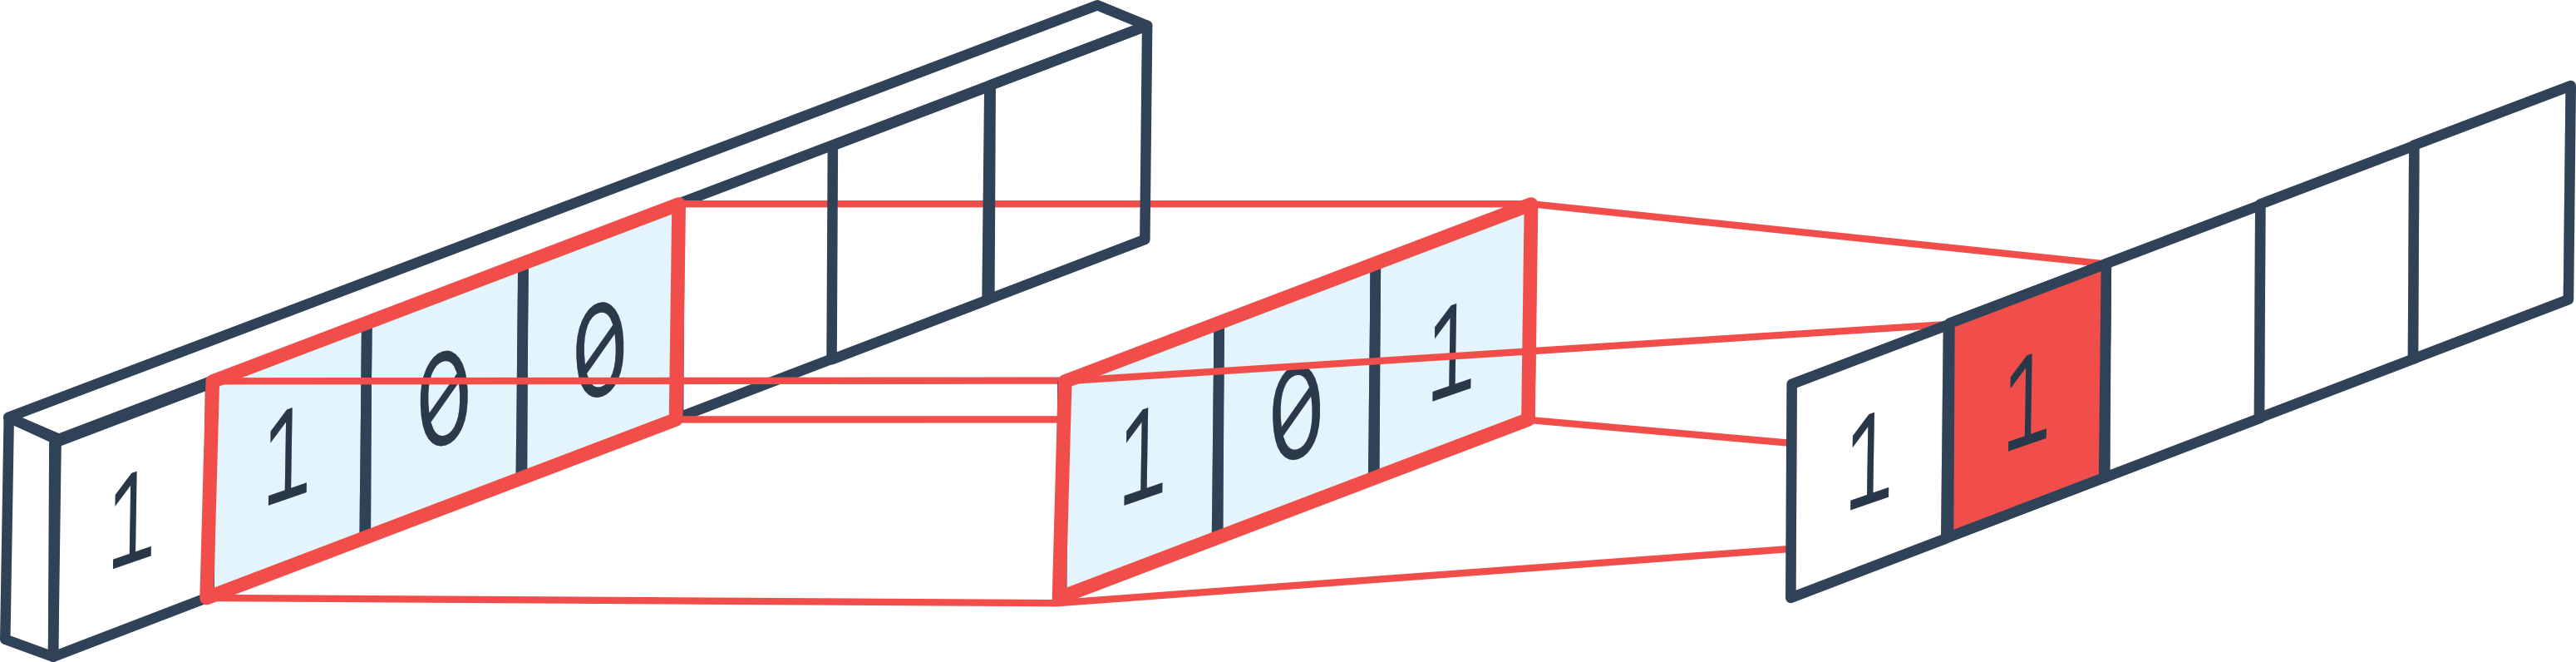
\includegraphics{1Dconv}
    \caption{A convolution in 1D space. Source:\url{https://peltarion.com/knowledge-center/documentation/modeling-view/build-an-ai-model/blocks/1d-convolution-block}}
    \labfig{conv}
\end{marginfigure}
The easiest example would be a 3x3 filter which blurs the image it is applied to.
The filter given in \reffig{conv_blur} results in such blurring since the signal of the pixel at the center is dominant but mixed with the signal of its surrounding pixels.
\begin{marginfigure}
    \setlength{\extrarowheight}{2pt}
    \begin{TAB}(2, 1cm, 1cm){|c|c|c|}{|c|c|c|}
        $\frac{1}{16}$ & $\frac{1}{8}$ & $\frac{1}{16}$ \\
        $\frac{1}{8}$ & $\frac{1}{4}$ & $\frac{1}{8}$ \\
        $\frac{1}{16}$ & $\frac{1}{8}$ & $\frac{1}{16}$ \\
    \end{TAB}
    \caption{3x3 filter for blurring (Gaussian Blur).}
    \labfig{conv_blur}
\end{marginfigure}

Another filter like \reffig{conv_sharp} will sharpen edges in an image since the signal of the surrounding pixels is subtracted from at the center pixel signal. 
\begin{marginfigure}
    \setlength{\extrarowheight}{2pt}
    \begin{TAB}(2, 1cm, 1cm){|c|c|c|}{|c|c|c|}
        $1$ & $0$ & $-1$ \\
        $2$ & $0$ & $-2$ \\
        $1$ & $0$ & $-1$ \\
    \end{TAB}
    \caption{3x3 filter for detecting edges in the y direction (Sobel filter).}
    \labfig{conv_sharp}
\end{marginfigure}

One can easily imagine that these kernels can also perform blurring only along one axis or sharpening gradients in one direction.
As many such filters are imaginable, there are often many filters applied per layer called filter-banks.
The output of each filter then defines an input channel for the next layer much like the three color channels in an image.
With many channels convolutions can become even more complex as each filter takes all previous channels as input and combines them into a new channel.\\
Interestingly, the weights of each kernel may not be hand-crafted but can be learned similar to fully connected layers.

As convolutions qualify as linear functions, there exists an equal fully connected layer to each convolutional layer.
The weights of such an FC layer would be sparse, though, which means there are many values equal to zero.
This property makes it clear that convolutions are more efficient than fully connected layers by imposing some simple restrictions.

Similar behavior also occurs when comparing convolutional layers with different kernel sizes.
By using a larger kernel, the ``field of view'' (the area that each pixel in the result layer ``sees'') increases as well.
At the same time, a larger kernel increases the number of parameters significantly.
\marginnote{A convolutional kernel with the size of the input would be equivalent to a fully connected layer.}
The same field of view can also be obtained, though, when using two convolutions in series.\\
\eg two layers with kernel size $3 \times 3$ have the same field of view like a single layer with kernel size $5 \times 5$ but fewer weights.

\subsection{Pooling}
A sub-type of convolutional layers are pooling layers.
Pooling layers have the purpose of downsampling an image or layer to a lower resolution.
Basically, downsampling can already be achieved by choosing a convolutional layer with stride $s > 1$.
Another way is to downsample an image without any learnable weights is by using one of two specific hand-crafted kernels.

The first option is average-pooling.
By taking the mean of four neighboring pixels (each weight is $\frac{1}{4}$) with a stride of $s = 2$ in each channel, the input is scaled down by a factor of $2$ along each axis.
Figuratively, four pixels will be combined into a single pixel by taking their mean.

On the other hand, max-pooling does not take the average but only takes the maximum value of the four inputs.
The result will then propagate only the most dominant signals.

Either way, pooling will result in loss of information but is often necessary to reduce the computational load.
Especially when the number of channels increases for deeper layers, it is preferable to reduce memory usage and computational load along with the spatial size.

Typical CNN architectures will often stack several convolutional layers then apply a single pooling layer.
Then another stack of convolutional layers is applied.
This way, the input's spatial size is gradually reduced, while the number of channels is increased at the same time.

\section{Recurrent Neural Networks}
All previously presented networks have in common that they generate simple outputs $y_i$ such as a class from simple inputs $x_i$ such as the frequency of a certain word.
In fact, images and even videos can act as inputs and outputs.
Nevertheless, the larger the output, the harder it is to train.
Recurrent neural networks are specialized for sequences of data as inputs and/or outputs.\\
Again, the email-spam problem can be manipulated such that a recurrent network fits the task.
The classifier should check whether an email classifies as spam by analyzing whether an email is well written or just a bunch of buzzwords.
Such an approach could be realized by taking the whole email as an input of an FC layer.
However, similar to how convolutional layers are more efficient than FC layers for images, are recurrent networks more efficient for sequences.

Instead of feeding a whole sentence at once, RNNs take only one word at a time as input.
Then the activation for a hidden layer is calculated and stored.
During the next part of the input sequence, the previously stored activations provide an additional input besides the sequence snippet.
Then new activations are generated, which are again stored for the next step of the sequence.
This process is repeated until the sequence is complete, and then an output is generated.

Recurrent neural networks are prevalent in natural language processing as language can easily be visualized as a sequence.

\section{Types of Learning}
Neural networks are often categorized into different groups.
One popular way of grouping is by categorizing the training according to the way the data is structured~\cite{grosse, ommer}.

\subsection{Supervised Learning}
If data is available, which already shows the network's desired behavior, training falls into the supervised learning category.
Referencing the previous example, this would mean that there are emails available that are already labeled as ``spam'' or ``not-spam''.
The network can then imitate this behavior from the data. \\
Most problems fall into the supervised category as they are also the easiest to solve~\cite{grosse}.

\subsection{Reinforcement Learning}
In reinforcement learning, there is no such paired data available.
However, the result can be evaluated how good it solves the problem.
The resulting score is called a reward.\\
Most AIs trained to play games such as Google Alpha Go~\cite{alphago} are based on reinforcement learning.
They also overcome the problem that calculating the reward is often based on undifferentiable outputs such as the score in a video game~\cite{grosse}.

\subsection{Unsupervised Learning}
Unsupervised learning has to deal with data that has no labels.
Usually, this means finding patterns in the data on its own~\cite{grosse}.
Considering the email-spam problem: A network is given all the email data without labels spam or not-spam.
Ideally, the network is then able to find patterns in emails which allow grouping these emails.
These groups are then evaluated, and hopefully, one group coincides with the ``spam'' label or any other desired label.

